%\documentclass[10pt,a4paper]{report}
\documentclass[10pt,a4paper]{report}

\usepackage{amsmath}
\usepackage{floatflt}
\usepackage{graphicx}
\graphicspath{{./figs/}}
\usepackage{subfig}
%\usepackage{wasysym}
%\usepackage{multicol}
%\usepackage[latin2]{inputenc}   
%\usepackage[T1]{fontenc}  
\usepackage[finalnew]{trackchanges} %finalnew, finalold, footnotes, margins, inlines
\usepackage{fancybox}
%\usepackage{subfigure}
\usepackage{wrapfig}
     
\setlength{\topmargin}{-0.5in}
\setlength{\textheight}{9in}
\setlength{\oddsidemargin}{-0.1in}
\setlength{\evensidemargin}{0.in}
\setlength{\textwidth}{6.5in}
\setlength{\headsep}{1.2cm}
\setlength{\parskip}{0.2cm}
\setlength{\parindent}{0.cm}

\newcommand{\uvec}[1]{\ensuremath{\underline{#1}}}
\newcommand{\beq}{\begin{equation}}
\newcommand{\eeq}{\end{equation}}

% Szurke keretezett kidolgozott feladat
\usepackage{tcolorbox}
\tcbuselibrary{skins,breakable}

\pagestyle{myheadings}    % Go for customised headings
\markboth{}{Fluid Machinery}
\newcounter{prob}
\setcounter{prob}{1}

\title{Fluid Machinery\\  Lecture notes }
\author{Csaba H\H{o}s\\ {\tt hos.csaba@gpk.bme.hu}\\
%
\vspace{1cm}\\
%
Budapest University of Technology and Economics\\
Dept. of Hydrodynamic Systems\\
%
\vspace{1cm}\\
%
with major contributaions by\\
Ferenc Heged\H{u}s, Csaba Bazs\'o, Rox\'ana Varga, Rich\'ard W\'eber}

\begin{document}
\maketitle
\tableofcontents

\input{chap1_thermodynamics}

% !TEX root = fluid_machinery_lecture_notes.tex
\chapter{Incompressible turbomachinery}

We classify as \emph{turbomachines} all those devices in which energy is transferred either to, or from, a continuously flowing fluid by the \emph{dynamic} action of one ore moving blase rows. Essentially, a rotating blade row, a rotor or an impeller changes the \emph{stagnation enthalpy} of the fluid moving through it. These enthalpy changes are intimately linked with the pressure changes in the fluid.

Up to 20\% relative density change, also gases are considered to be incompressible. Assuming isentropic process and ideal gas, this corresponds to $p_2/p_1 \approx 1.3$. Thus, pumps, fans, water and wind turbines are essentially the same machines.

\section{Euler's turbine equation}

Euler's turbine equation (sometimes called Euler's pump equation) plays a central role in turbomachinery as it connects the specific work $Y$ and the geometry and velocities in the impeller. In what follows, we give two derivations of the equation.

\begin{figure}[ht]
\begin{center}
\includegraphics[scale=0.5]{figs/euler_turbine_equation_fig.png}
\caption{\label{gen_turbom}Generalized turbomachine}
\end{center}
\end{figure}

{\bf Derivation 1: Moment of momentum}

Let us compute the moment of the force that is applied at the inlet and outlet of the generalized turbomachine shown in figure \ref{gen_turbom}:

\begin{equation}
\uvec{F}=\frac{\mathrm{d}}{\mathrm{d} t}\left( m \uvec{c}\right)
\quad \rightarrow\quad
\uvec{M}=\frac{\mathrm{d}}{\mathrm{d} t}\left( \uvec{r} \times m \uvec{c}\right)=\dot{m}\left( \uvec{r} \times \uvec{c}\right)
\end{equation}

where $m$ is the mass flow, and $\underline{c}$ is the velocity of the fluid on the radius $r$. We consider the following assumptions:
\begin{itemize}
  \item The inlet of the turbomachine is a circle with radius $r_1$, and the outlet with radius $r_2$.
  \item $\underline{c}$ velocity is considered constant in the sense that its length and angle are constant.
\end{itemize}
Thus $$ \uvec{M} = \uvec{M}_{out}-\uvec{M}_{in}=\dot{m}\left( \uvec{r}_2 \times \uvec{c}_2\right) - \dot{m}\left( \uvec{r}_1 \times \uvec{c}_1\right) $$.
With this the power need of driving the machine is
%
\begin{eqnarray}
	\dot m Y &= & P = \uvec{\omega} \uvec{M} = \left(\uvec{M}_{out}-\uvec{M}_{in}\right)\, \uvec{\omega}
	=\dot m \left[ \uvec{\omega} \left( \uvec{r}_2 \times \uvec{c}_2\right) - \uvec{\omega} \left( \uvec{r}_1 \times \uvec{c}_1\right) \right] \nonumber\\
	&=&\dot m \left[ \uvec{c}_2 \left( \uvec{\omega} \times \uvec{r}_2 \right) - \uvec{c}_1 \left( \uvec{\omega} \times \uvec{r}_1 \right) \right]
	=\dot m \left[ \uvec{c}_2 \uvec{u}_2 - \uvec{c}_1 \uvec{u}_1 \right] \nonumber\\
	&=&\dot m \left[ |\uvec{c}_2| |\uvec{u}_2| - |\uvec{c}_1| |\uvec{u}_1| \right]
	=\dot m \left( c_{2u} u_2 - c_{1u} u_1\right)
\end{eqnarray}
%
where $u_i = |\uvec{u}_i|$, and $c_i=|\uvec{c}_{2u}| cos(\alpha)$.
Comparing the beginning and the end of the equation, we see that the specific work is
\begin{equation}
\boxed{Y=c_{2u} u_2 - c_{1u} u_1}.
\end{equation}

{\bf Derivation 2: Rotating frame and reference and rothalpy}

The Bernoulli equation in a rotating frame of reference reads
%
\beq
\frac{p}{\rho}+\frac{w^2}{2}+U = \mathrm{const.},
\eeq
%
where $U$ is the potential associated with the conservative force field, which is the potential of a rotating frame for reference: $U=-r^2\omega^2/2$. Let $w$ stand for the relative velocity, $c$ for the absolute velocity and $u=r \omega$ for the 'transport' velocity. We have $\uvec{c}=\uvec{u}+\uvec{w}$, thus $w^2=u^2+c^2-2u\,c=u^2+c^2-2u\,c_u$, which gives
\begin{equation}
\frac{p}{\rho}+\frac{w^2}{2}-\frac{r^2 \omega^2}{2}=\frac{p}{\rho}+\frac{c^2+u^2-2c u}{2}-\frac{u^2}{2}=\frac{p}{\rho}+\frac{c^2}{2}-\underbrace{c\,u}_{c_u u}=\mathrm{const}.
\end{equation}

Thus we see that the above quantity is conserved in a rotating frame of reference, which we refer to as \emph{rothalpy} (abbreviation of rotational enthalpy). Let us find now the change of energy inside the machine:
%
\begin{equation}
Y=\Delta \left(\frac{p}{\rho}+\frac{c^2}{2}\right)=\Delta \left( c_u u\right),
\end{equation}
%
which is exactly Euler's turbine equation. (For compressible fluids, rothalpy is $I=c_p T+\frac{c^2}{2}-u c_{u}$.)

\section{Velocity triangles and performance curves} \label{sec:velocity_triangles_pumps}

% \begin{figure}[ht]
% 	\begin{center}\label{fig:velcoitytriangles}
% 		%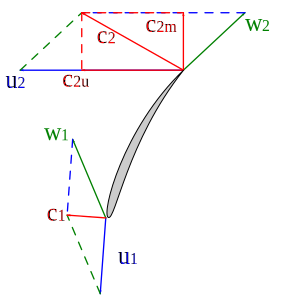
\includegraphics[scale=0.5]{figs/VelocityTriangles.png}
% 		%\includegraphics[scale=0.5]{Impeller3D_and_VelocityTriangles_v2.png}
% 		\includegraphics[width=0.8\textwidth]{Impeller2D_and_VelocityTriangles.png}
% 		\caption{Velocity triangles at the inlet and at the outlet}
% 	\end{center}
% \end{figure}

% \note{VelocityTriangle figure added by Weber Richard}
From the Euler turbine equation we have:
%
\begin{equation*}
  \Delta p_e = \rho g H = \rho \left( c_{2u}u_2 - c_{1u}u_1 \right)
\end{equation*}
%
where $H$ is the head of the pump. Known the velocity triangle's components and the density of the fluid, we get:
%
\begin{equation}\label{radial_head}
  H = \frac{c_{2u}u_2 - c_{1u}u_1}{g}
\end{equation}
%
The volume flow rate is
\begin{equation}\label{radial_flow}
  Q = c_{2m} A_2 =c_{2m} D_2 \pi b_2,
\end{equation}
%
where $D_2$ is the impeller outer diameter, $b_2$ is its flow-through width at the outlet. From \ref{radial_head} and \ref{radial_flow} we have that $\uvec{c}$ outlet absolute velocity is the connection between the head and the flow rate of the pump. Also one can notice, that if $ \Delta p_e$ increased, that is when $c_{2u}$ is increased than $Q$ decreases ($c_{2m}$ decreases). And if $\Delta p_e$ decreased ($c_{2u}$ decreased) than $Q$ increases ($c_{2m}$ increases). So our goal now is to find a relationship between the head and the flow rate of the pump.

\subsection{Radial (centrifugal) machines}

Let us consider a centrifugal pump and the velocity triangles at the impeller inlet and outlet, see Fig. \ref{fig:centrifual_pumps}. The theoretical volume flow rate is
%
\begin{equation}
Q_{th}=c_{2m} A_2 \Psi =c_{2m} D_2 \pi b_2 \Psi,
\end{equation}
%
where $D_2$ is the impeller outer diameter, $b_2$ is its flow-through width at the outlet and $c_{2m}$ is the radial component of the outlet absolute velocity. $\Psi<1$ is a constant called \emph{blockage factor} that takes into account that the real flow through area is smaller due to the blockage of the blade width at the outlet.

\begin{figure}[ht]
\begin{center}
\includegraphics[width=0.52\textwidth]{figs/Centrifugal_Pump.png}
%\includegraphics[width=0.45\textwidth]{figs/Double-Suction-Centrifugal-Pump.jpg}
\caption{\label{fig:centrifual_pumps}Centrifugal pumps}
\end{center}
\end{figure}

%\begin{minipage}{\textwidth}

%\begin{floatingfigure}[r]{0.5\textwidth}
%\begin{center}
%\includegraphics[width=0.35\textwidth]{figs/Impeller3D_and_VelocityTriangles.png}
%\caption{\label{fig:centrifual_pumps_velocity_triangle}Centrifugal impeller with outlet velocity components.}
%\end{center}
%\end{floatingfigure}

\begin{figure}[ht]
\begin{center}
\includegraphics[width=6cm]{figs/Impeller3D_and_VelocityTriangles_v2.png}
\hspace{0.5cm}
\includegraphics[width=7.5cm]{figs/Impeller2D_and_VelocityTriangles.png}
\caption{\label{fig:centrifual_pumps_velocity_triangle}Centrifugal impeller with outlet velocity components.}
\end{center}
\end{figure}

The velocity triangle describes the relationship between the absolute velocity $c$, the circumferential velocity $u$ and the relative velocity $w$. Obviously, we have $\vec{c}=\vec{u}+\vec{w}$. Moreover, we know that (a) the circumferential velocity is $u=D \pi n$ and that (b) the relative velocity is tangent to the blade, i.e. the angle between $u$ and $w$ is approximately the blade angle $\beta$.

Basic trigonometrical identities show that $c_{2u}=u_2-c_{2m}/\tan \beta_2$. It is usual to assume that the flow has no swirling (circumferential) component at the inlet (due to Helmholtz's third theorem). In the reality, the outlet flow angle is not exactly $\beta_2$, thus the head is decreased, which is taken into account with the help of the \emph{slip factor} $\lambda$ (sometimes denoted by $\sigma$ in the literature).
%\end{minipage}

If there is no \emph{prerotation} (i.e. $c_{1u}=0$), we have
%
\begin{align}
H_{th}&=\lambda \frac{c_{2u} u_2}{g}=\lambda\left(\frac{u_2^2}{g}-\frac{u_2}{g}\frac{w_{2u}}{g}\right)=\lambda\left(\frac{u_2^2}{g}-\frac{u_2}{g}\frac{c_{2m}}{\tan \beta_2}\right)\nonumber \\
&=\lambda\left(\frac{u_2^2}{g}-\frac{u_2}{g\tan \beta_2 D_2 \pi b_2 \Psi}Q_{th}\right).
\end{align}

Thus, the theoretical performance curve $H_{th}(Q_{th})$ of a centrifugal machine is a straight line, which is (see Figure \ref{fig:blade_shapes})
\begin{itemize}
\item decreasing as $Q$ is increased, for \emph{backward curved} blades, i.e. $\beta_2<90^o$,
\item horizontal, for \emph{radial blades} ($\beta_2=90^o$) and
\item increasing (as $Q$ is increased) for \emph{forward curved} blades, i.e. $\beta_2>90^o$.
\end{itemize}

\begin{figure}[ht]
\begin{center}
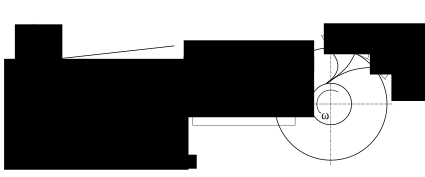
\includegraphics[width=0.8\textwidth]{figs/RadialPump_BladeShapes.png}
\caption{\label{fig:blade_shapes}Effect of blade shapes $\beta_2$ angle on the performance curve.}
\end{center}
\end{figure}

\subsection{Problems}

\noindent {\bf Problem \thesection.\theprob}\stepcounter{prob} 

A radial impeller runs at n=1440/min revolution speed and conveys $Q=40$ l/s of water. The diameter of the impeller is $D= 240$ mm, the outlet width is $b_2=20$ mm. The blade angle at the outlet is $\beta_2 = 25$ degrees. The inlet is prerotation-free. Find the theoretical head and draw a qualitatively proper sketch of the velocity triangle at the outlet. (Solution: $H_{th}=22.9$m)

\vspace{1cm}
\noindent {\bf Problem \thesection.\theprob}\stepcounter{prob}

The mean meridian velocity component of a radial impeller with $D_2=400$ mm diameter at $n=1440$rpm revolution speed is $c_m= 2.5$ m/s. The angle between the relative and circumferential velocity components is $\beta_2=25$ degrees. With a geometrical change of the blade shape, this angle is increased to to 28 degrees, that results in 10\% drop of the meridian velocity component. The inlet is prerotation-free. Find the relative head change. (Solution: $(H_{25^o}-H_{28^o})/H_{25^o}=4.6$\%) 



\subsection{Axial machines}

In the case of axial machines the flow leaves the impeller axially, see Fig. \ref{fig:axial_pumps}. The flow-through area is $\left(D_o^2-D_i^2\right)\pi/4$, where $D_o$ and $D_i$ stand for the outer and inner diameter of the lade, respectively. Notice that in this case, $u_1=u_2$ because it is assumed that the flow moves along a constant radius. Assuming (again) prerotation-free inlet ($c_{1u}=0$), we have $c_{2m}=c_1$ (due to continuity).

\begin{figure}[ht]
\begin{center}
\includegraphics[width=0.3\textwidth]{figs/axial_pump1.jpg}
\hspace{1cm}
\includegraphics[width=0.3\textwidth]{figs/axialfanplate.jpg}
\caption{\label{fig:axial_pumps}Axial pump (left) and axial fan (right)}
\end{center}
\end{figure}

However, an important difference between axial and centrifugal pumps (fans) is that in the case of axial machines, the pressure rise changes along the radial coordinate of the blade:
%
\beq
\Delta p_t(r)=\left.\rho u(r) \left(c_{2u}(r)-c_{1u}(r) \right)\right|_{c_{1u}=0}=\rho \left( 2 r \pi n \right) \left(2 r \pi n-\frac{c_{2m}}{\tan \beta_2} \right).
\eeq
%
Thus, if we wanted to obtain \emph{constant} $\Delta p_t$ along the radial coordinate, the change of the circumferential velocity has to be compensated by varying $\beta_2$.

\begin{figure}[ht]
\begin{center}
\includegraphics[width=0.3\textwidth]{figs/AxialPump_axon.png}
\hspace{1cm}
\includegraphics[width=0.3\textwidth]{figs/AxialPump_side.png}
\caption{\label{fig:axial_machines}Axial impeller with outlet velocity components.}
\end{center}
\end{figure}

%\begin{minipage}{\textwidth}
%
%\begin{floatingfigure}[r]{0.5\textwidth}
%\centering
%\includegraphics[width=0.45\textwidth]{figs/WorldWarWoodenPropeller.jpg}
%\caption{\label{fig:propeller}World War I wooden propeller}
%\end{floatingfigure}
%
%The twisted airfoil (aerofoil) shape of modern aircraft propellers was pioneered by the Wright brothers. While both the blade element theory and the momentum theory had their supporters, the Wright brothers were able to combine both theories. They found that a propeller is essentially the same as a wing and so were able to use data collected from their earlier wind tunnel experiments on wings. They also found that the relative angle of attack from the forward movement of the aircraft was different for all points along the length of the blade, thus it was necessary to introduce a twist along its length. Their original propeller blades are only about 5\% less efficient than the modern equivalent, some 100 years later. (Source: Wikipedia)
%
%\end{minipage}

\subsection{Problems}
\begin{tcolorbox}
\noindent {\bf Problem \thesection.\theprob}\stepcounter{prob}

The outer diameter of a CPU axial cooler ventilator is $D_o=47\,\mathrm{mm}$ the inner diameter is $D_i=21.5\,\mathrm{mm}$ the revolution speed is $n=2740\,\mathrm{rpm}$. Due to the careful design the hydraulic efficiency is $\eta_h=85\%$ however the volumetric efficiency as consequence of leakage flow rate between the housing and the impeller is just $\eta_{vol}=75\%$. The blade angle at the suction side is $\beta_1=20^\circ$ while at the pressure side $\beta_2=40^\circ$. Find the flow rate and the total pressure rise on the impeller. The density of the air is $\rho=1.25\,\mathrm{kg/m^3}$. Draw the velocity triangles at the inlet and the outlet at the mean diameter.
%
\begin{itemize}
\item $A_{ring}=\frac{\left(D_o^2-D_i^2\right)\pi}{4}=0.00137\,\mathrm{m^2}$
\item $D_{mean}=\frac{D_o+D_i}{2}=0.03425\,\mathrm{m}$
\item $u_{mean}=u_1=u_2=D_{mean}\pi n=4.913\,\mathrm{\frac{m}{s}}$
\item $c_{ax}=c_{1,ax}=c_{2,ax}=u \tan\beta_1=1.788\,\mathrm{\frac{m}{s}}$
\item $q=\eta_{vol}A_{ring}c_{ax}=0.00184\,\mathrm{\frac{m^3}{s}}$
\item $w_{2u}=\frac{c_{ax}}{\tan\beta_2}=2.131\,\mathrm{\frac{m}{s}}$
\item $\Delta c_u=u-w_{2u}=2.782\,\mathrm{\frac{m}{s}}$
\item $\Delta p_{total,ideal}=\rho u\Delta c_u=17.1\,\mathrm{Pa}$
\item $\Delta p_{total}=\eta_h \Delta p_{total,ideal}=14.5\,\mathrm{Pa}$
\end{itemize}
\end{tcolorbox}
	
\vspace{1cm}
\begin{tcolorbox}
\noindent {\bf Problem \thesection.\theprob}\stepcounter{prob}

The inner diameter of an axial impeller is $D_i=250$ mm, while the outer one is $D_o=400$mm. The revolution number of the impeller is $1470$rpm. The inlet is prerotation-free. At $Q=0.36\,\mathrm{ m^3/s}$ the hydraulic efficiency is 85\%, the head is 6 m. The specific work along the radius is constant. Find the angles $\beta_{1,2}$  at the inner and outer diameter. 


%(Solution: $\beta_{1,i}=13.7$, $\beta_{2,i}=16.7$, $\beta_{1,o}=8.7$ and $\beta_{2,o}=9.4$ degrees) 
\vspace{0.2cm}

Solution:

\begin{itemize}
%
\item The velocity triangles are depicted in the Figure \ref{gen_vtr}.
%
\item The circumferential speed at the inner diameter is $u_{2i}=D_i\pi n=0.25\pi \frac{1470}{60}= 19.24 m/s$. The two circumferential speeds $u_{i,1}$ and $u_{i,2}$ equal as they are located at the same (inner) radius.
%
\item The circumferential speed at the outer diameter is $u_{20}=D_o\pi n=0.4\pi\frac{1470}{60}= 30.79 m/s$. Again the the two circumferential speeds $u_{o,1}$ and $u_{o,2}$ equal as they are located at the same (outer) radius.
%
\item The theoretical head is $H_{th}=\frac{c_{2u}u_2}{g}=\frac{H}{\eta_h}=7.059m$. We also have  $c_{2u}u_2=H_{th}g=69.247$ $m^2/s^2$, which is constant along the radius: $c_{2u,i}=\frac{69.247}{19.24}=3.56$ m/s and $c_{2u,o}=\frac{69.247}{30.79}=2.25$ m/s.
%
\item The axial component of the velocity is $c_{ax}=\frac{4Q}{\left({D_o}^2-{D_i}^2\right)\pi}=\frac{4 \times 0.36}{\left({0.4}^2-{0.25}^2\right)\pi}=4.70$ m/s
%
\item The blade angles are
\begin{equation*}
\beta_{1i}=\arctan\frac{c_{ax}}{u_{2i}}=
%=\arctan\frac{4.70}{19.24}=
13.73^o \quad \text{and}\quad \beta_{2i}=\arctan\frac{c_{ax}}{u_{2a}-c_{2ui}}
%=arctan\frac{4.70}{19.24-3.56}=
=16.7^o.
\end{equation*}

\item With the same train of thought, one obtains $\beta_{10}=8.7^o$ and $\beta_{20}=9.4^o$.
\end{itemize}
\end{tcolorbox}
\vspace{1cm}

\begin{figure}[ht]
\begin{center}
\includegraphics[scale=0.6]{figs/problem_2p2p16_vel_tri_fig.png}
\caption{\label{gen_vtr}Velocity triangles}
\end{center}
\end{figure}



\clearpage

\subsection{Real performance curves} \label{sec:real_performance_curves_turbomachines}

Our analysis so far assumed that the flow inside the impeller is ideal (no losses) and that the streamlines are following the blade shape (thus, blade angles are also the streamline angles). However neither of these assumptions are true.

There are significant friction losses inside the impeller, the narrower the flow passage is, the higher the friction losses will be. Moreover, the volute also introduces friction losses. These losses are proportional to the velocity squared, thus $H'_{friction} \propto Q^2$.

On the other hand, if the angle of attack deviates from the ideal one, one experiences separation on the two sides of the blade. This is illustrated in Figure~\ref{fig:real_perf_curve} for a constant circumferential velocity $u$ as the flow rate and thus the inlet velocity $c$ is varied, the relative velocity $w$ also varies. At the design flow rate $Q_d$ the angle of attack ideal. For small flow rates, we have separation on the suction side of the blade, while for larger flow rates the separation is on the pressure side of the blade. Thus we have $H'_{separation} \propto (Q-Q_d)^2$.

To obtain the real performance curve, one has to subtract the above two losses from the theoretical head: $H=H_{th}(Q)-K_1 Q^2-K_2 (Q-Q_d)^2$, which is illustrated in \ref{fig:real_perf_curve}. Note that at the design point and close to it, the friction losses are moderate and no separation occurs. For lower flow rates, the friction loss decreases while separation increases. For higher flow rates, both friction and separation losses increase.

\begin{figure}[ht]
\centering
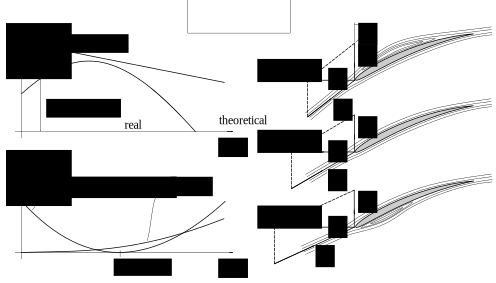
\includegraphics{figs/HeadLosses.png}
\caption{\label{fig:real_perf_curve}Friction and separation losses in the impeller.}
\end{figure}

%%%%%%%%%%%%%%%%%%%%%%%%%%%%%%%%%%%%%%%%%%%%%%%%%%%%%%%%%%%%%%%%%%%%%%%%%%%%%%%%%%%%%%%%%%%%%%%

\clearpage

\section{Losses and efficiencies}

Let us analyse the losses that decrease the efficiency of a turbomachine (see Figure~\ref{fig:PumpLosses}).

\begin{figure}[ht]
\centering
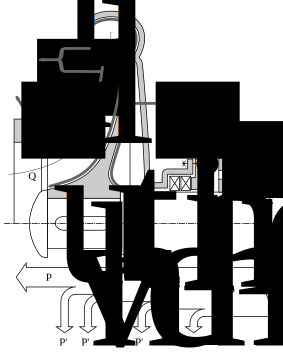
\includegraphics{figs/PumpLosses.png}
\caption{\label{fig:PumpLosses}Losses of the pump.}
\end{figure}

\noindent Let the input mechanical power transmitted by the shaft be denoted by $P_{input}$. We have than

\begin{description}
\item[Mechanical losses $P'_m$] These represent the friction loss in the bearings and the mechanical sealing losses (if any). The remaining power is called \emph{internal power} $P_i=P_{input}-P'_m$.
%
\item[Disc friction losses $P'_{df}$] A significant shear force appears in the fluid entrapped between the housing and the impeller, which is taken into account by the \emph{disc friction coefficient}: $P'_{df}=\nu_{df} P_i$. The remaining power is the theoretical power of the impeller: $P_{th}=P_i-P'_{df}=(1-\nu_{df}) P_i$.
%
\item[Hydraulic and volumetric losses $P'_h$, $P'_v$] The theoretical head $H_{th}$ and flow rate $Q_{th}$ and is further decreased by the leakage flow rates ($Q_{l(eakage)}$) inside the pump (flow across the gaps between the impeller and the housing) and the internal frictional losses $h'$ (e.g. in the impeller and volute). We have
\begin{align}
P_{th}&=Q_{th} \rho g H_{th}=\left( Q+Q_{l}\right) \rho g \left( H+h'\right)=\underbrace{Q \rho g H}_{P_{u}}+\underbrace{Q_l \rho g H}_{P'_v}+\underbrace{Q_{th}\rho g h'}_{P'_h}\nonumber\\
&=Q\rho g H \frac{Q+Q_{l}}{Q}\frac{H+h'}{H}=Q\rho g H \underbrace{\frac{Q_{th}}{Q}}_{\eta_v^{-1}} \underbrace{\frac{H_{th}}{H}}_{\eta_h^{-1}} \quad \rightarrow \quad P_u=P_{th}\eta_h \eta_v
\end{align}
\end{description}

\newpage
\subsection{Problems}


\begin{tcolorbox}
\noindent {\bf Problem \thesection.\theprob}\stepcounter{prob}

The revolution number of a water pump is 1470 rpm, the flow rate is $Q=0.055\mathrm{m^3/s}$ and the head is $H=45$m. The hydraulic power loss is $P'_h=2.5$kW, the mechanical power loss is $P'_m=1.3$kW, the disc friction coefficient is $\nu_t=0.065$. The input power at this operating point is $P_{in}=32$kW. Make a complete analysis of the losses, including leakage flow rate and the theoretical head.

\noindent Solution:

The power flow chart is in Figure \ref{gen_pfc}

\begin{itemize}
\item $P_{i}=P_{input}-P'_{m}=30.7\,\mathrm{kW}\quad \rightarrow \quad \eta_{m}=95.9\%$
\item $P_{th}=(1-\nu)P_{i}=28.7\,\mathrm{kW}$
\item $h'_{h}=\frac{P'_{h}}{\rho g Q}=4.63\,\mathrm{m} \quad \rightarrow \quad H_{th}=45+4.63=49.63\,\mathrm{m}\quad \rightarrow \quad \eta_{hydr}=90.6\%$
\item $Q_{th}=\frac{P_{th}}{\rho g H_{th}}=0.0589\,\mathrm{m^3/s}\quad \rightarrow \quad Q_{leakage}=0.00395\,\mathrm{m^3/s}\quad \rightarrow \quad \eta_{v}=93.2\%$ 
\item $\eta_{overall}=\eta_{v} \cdot\eta_{h} \cdot (1-\nu) \cdot \eta_{m} = 75.9\%$
\end{itemize}
\end{tcolorbox}
\vspace{1cm}

\begin{figure}[ht]
\begin{center}
\includegraphics[scale=0.85]{figs/problem_2p3p17_pow_flow_chart_fig.png}
\caption{\label{gen_pfc}Power flow chart}
\end{center}
\end{figure}

\vspace{1cm}
\noindent {\bf Problem \thesection.\theprob}\stepcounter{prob}

\note{problem added by Weber Richard}
Calculate the theoretical head, the theoretical volume flow rate, the hydraulic efficiency and the volumetric efficiency based on the data of the water pump. $P_{input} = 43.5\,kW,$ $Q = 1100\,dm^3/min,$ $H = 180\,m,$ $P'_{mech} = 1.6\,kW,$ $\nu_{df} = 0.03, h' = 32\,m$.
(Solution: $H_{th} = 212\,m,$ $Q_{th} = 0.01954\,m^3/s$ $\eta_{hydr} = 84.9\%$ $ \eta_{vol} = 93.8\%$)

%----------------------------------------------------------------------------
\clearpage
\section{Dimensionless numbers and affinity} \label{sec:dimensionless_numbers}

Based on the previously obtained formulae for theoretical head, we define dimensionless numbers as
\beq
H=\eta_h H_{th}=2 \eta_h \frac{c_{2u}}{u_2}\frac{u_2^2}{2g}:=\psi \frac{u_2^2}{2g}
\eeq
%
or, in the case of fans
\beq
\Delta p_t=\psi \frac{\rho }{2}u_2^2,
\eeq
%
where $\psi$ is a dimensionless pressure rise. Similarly, we have
%
\beq
Q=\eta_v Q_{th}=\eta_v D_2 \pi b_2 c_{2m}=\eta_v \frac{4 D_2 \pi b_2}{4 D_2^2} \frac{c_{2m}}{u_2} u_2 D_2^2:=\varphi \frac{D_2^2 \pi}{4}u_2
\eeq

These dimensionless quantities are called \emph{pressure number} $\psi$ and \emph{flow number} $\varphi$. What we found is that $H \propto n^2$ and $Q \propto n$ allowing the transformation of the performance curve given at $n_1$ to be computed to another revolution number $n_2$. This is called \emph{affinity law}:
%
\beq
\frac{H_1}{H_2}=\left( \frac{n_1}{n_2}\right)^2, \quad \frac{Q_1}{Q_2}=\frac{n_1}{n_2} \quad \rightarrow \quad \frac{P_1}{P_2}=\left( \frac{n_1}{n_2}\right)^3
\eeq

As we have seen, both $\psi$ and $\varphi$ contains two parameters, $D_2$ and $u_2$, out of which one can be eliminated, resulting in new dimensionless numbers. Let us start with the elimination of $D_2$.
%
\begin{align}
\varphi&=\frac{Q}{\frac{D_2^2 \pi}{4}u_2}=\frac{4 Q}{D_2^3 \pi^2 n}\\
\psi&=\frac{H}{ \frac{u_2^2}{2g}}=\frac{2g H}{ D_2^2 \pi^2 n^2}
\end{align}
%
from which we have
%
\beq
\sigma=\frac{\varphi^{1/2}}{\psi^{3/4}}=\frac{2 \sqrt{Q}}{D_2^{3/2} \pi \sqrt{n}}\frac{ D_2^{3/2} \pi^{3/2} n^{3/2}}{\left(2g H\right)^{3/4}}=\frac{\sqrt{\pi}}{\sqrt[4]{2} g^{3/4}} \underbrace{n \frac{Q^{1/2}}{H^{3/4}}}_{n_q}
\eeq
%
Note that $\sigma$ depends only on the revolution number but takes different values along the performance curve. Thus when actually computing it, one takes the data of the best-efficiency point. Moreover, we do not include the constant term$ \frac{\sqrt{\pi}}{\sqrt[4]{2} g^{3/4}}$. Finally, by definition, the \emph{specific speed} of a turbomachine is

\beq
n_q=n[rpm]\frac{\left(Q_{opt.}[m^3/s]\right)^{1/2}}{\left(H_{opt.}[m]\right)^{3/4}}
\eeq

Specific speed defines the shape of the impeller, low specific speed means low flow rate and high pressure rise (radial impeller) while high specific speed occurs when the flow rate is high and the pressure rise is low, see Fig. \ref{fig:nq}.

\begin{figure}[ht]
\begin{center}
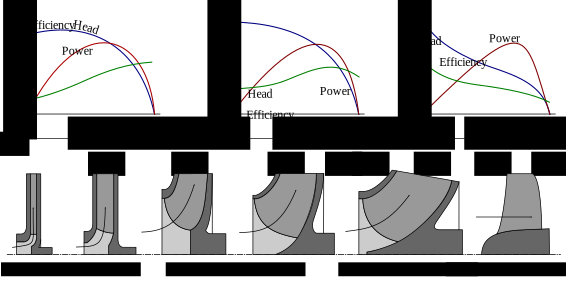
\includegraphics[width=0.8\textwidth]{figs/nq_eng.png}
\caption{\label{fig:nq}Specific speed and shape of the impeller.}
\end{center}
\end{figure}

Based on experience the available maximum efficiency can be estimated in the knowledge of $Q_{opt}$ and $n_q$ as follows

\beq
\eta_{max}=0.94-0.048 Q_{opt}^{-0.32}-0.29 \left(\log\left(\frac{n_q}{44}\right)\right)^2.
\eeq

Representing $\delta_{opt}(\sigma_{opt})$, turbomachines having good efficiency pass a narrow path. This diagram is called \emph{Cordier-diagram}. The centre of the path can be assumed with

\beq
\delta=\left(\frac{2.1}{1.41\log(\sigma)}\right)^{1.34}.
\eeq

Experience moreover shows that for a given $n_q$ estimation can be given for the ideal value of $\psi$ as follows

\beq
\psi=\left(\frac{300}{270+n_q}\right)^{9/4}.
\eeq


\subsection{Problems}

\noindent {\bf Problem \thesection.\theprob}\stepcounter{prob}

The input mechanical power of a water pump is 25 kW, the revolution number is 1440 rpm, the flow rate is 0.06 $\mathrm{m^3/s}$. The volumetric efficiency is estimated as $\eta_v=0.92$, the hydraulic efficiency is $\eta_h=0.85$, the disc friction power loss is $P'_{df}=0.9$ kW, the mechanical loss is $P'_m=1.3$ kW. Find the head and the specific speed and make a sketch of the impeller. (Solution: H=30.3m, $n_q$=27.3, the impeller is a thin radial one.)

%%%%%%%%%%%%%%%%%%%%%%%%%%%%%%%%%%%%%%%%%%%%%%%%%%%%%%%%%%%%%%%%%%%%

\vspace{1cm}
\noindent {\bf Problem \thesection.\theprob}\stepcounter{prob}

The revolution number of a pump is 1450 rpm, the head and flow rate at the best-efficiency point are 17m and 0.03 $\mathrm{m^3/s}$. Find the specific speed. Find the diameter of the impeller if, based on industrial experience, the pressure number at the best-efficiency point should be $\psi=1$. Find the flow number $\varphi$. Find the head and flow rate at 970rpm. (Solution: $n_q=30$, $D_2=240$mm, $\varphi=0.036$, $Q_{970\mathrm{rpm}}=0.02\mathrm{m^3/s}$, $H_{970\mathrm{rpm}}=7.61\mathrm{m}$) 

%%%%%%%%%%%%%%%%%%%%%%%%%%%%%%%%%%%%%%%%%%%%%%%%%%%%%%%%%%%%%%%%%

\vspace{1cm}
\noindent {\bf Problem \thesection.\theprob}\stepcounter{prob}

The head produced by a six stage pump type CR 8-60 is $H[m] = 68-0.2Q^2$, the speed of rotation is $n=2850~\frac{1}{\mathrm{min}}$. The efficiency is $\eta = 0.66-0.00731 (Q-9.5)^2$. The unit of the flow rate in the formulae is $[m3/h]$. Find the specific speed. Based on the specific speed, find the type of the impeller. Determine the input power of the water delivering pump for zero delivery $Q=0$ by extrapolation from calculated points in the range $Q = 1.5; 1; 0.5 m3/h$, and using L'Hopital's rule. (Solution: $n_q=29.9$, hence the impeller is radial; $P_{in}=1334W$.)

%%%%%%%%%%%%%%%%%%%%%%%%%%%%%%%%%%%%%%%%%%%%%%%%%%%%%%%%%%%%%%%%%

\vspace{1cm}
\begin{tcolorbox}
\noindent {\bf Problem \thesection.\theprob}\stepcounter{prob}

The characteristic curve of a pump at $n_1 = 1450/min$ rotor speed is $H_1 = 40m-40000s^2/m^5 Q^2$. Calculate 5 points of the pump-characteristic for the rotor speed $n_2 = 2900/min$ in the flow rate range $Q_2 = 0,01m^3/s-0,05m^3/s$ at $0,01 m^3/s$ intervals. According to laboratory tests the affinity law is valid in this range. Give the equation of the characteristics $H_2(Q_2)$ for the rotor speed $n_2$! (Solution: $H_2(Q_2)=160-40000Q_{2}^{2}$)
\vspace{0.2cm}

Solution:
\vspace{0.2cm}

{\bf Affinity laws:}

\begin{equation*}
	\frac{q_2}{q1}=\frac{n_2}{n_1}=2, \quad
	\frac{H_2}{H_1}=\left(\frac{n_2}{n_1}\right)^2=2^2=4
	\quad \text{and} \quad \frac{P_2}{P_1}=\left(\frac{n_2}{n1}\right)^3=2^3=8.
\end{equation*}
\vspace{0.2cm}

\begin{center}
\begin{tabular}{|c|c|c|c|c|c|c|c|}
	\hline
2.with affinity & $q_1 =q_2/2[m^3/s]$ & 0 & 0.005 & 0.01 & 0.015 & 0.02  & 0.025 \\
	\hline
3.with the caracteristic curve	& $H_1$[m] & 40 & 39 & 36 & 31 & 24 & 15 \\
	\hline
1.given & $q_2$ $[m^3/s]$ & 0 & 0.01 & 0.02 & 0.03 & 0.04 & 0.05 \\
	\hline
4.with affinity	& $H_2=4H_1$ & 160 & 156 & 144 & 124 & 96 & 60 \\
	\hline
\end{tabular}
\end{center}

\vspace{0.2cm}

{\bf Conversion of the characteristic curve analytically}

the general shape of the characteristic curve of a pump at n1 speed: $H_1=A+Bq+Cq^2$ (n this case we assumed that the characteristic curve H(q) of a pump can be described with a second degree polynomial. In reality this is a good approximation). In the present problem, the linear term (Bq) is zero.

\begin{equation*}
	H_1=A+Bq+C^2q=A+C^2q.
\end{equation*}
%(Of course, if in another task, in the case of another pump, B $\ne$ 0, the following derivation can also be performed)
%Derivation:
%
We have:
%
\begin{equation*}
	H_2=H_1\left(\frac{n_2}{n_1}\right)^2=\left(\frac{n_2}{n_1}\right)^2\left(A+C{q_1}^2\right)=1\left(\frac{n_2}{n_1}\right)^2\left[A+C{q_2}^2\left(\frac{n_1}{n_2}\right)^2\right]=A\left(\frac{n_2}{n_1}\right)^2+C{q_2}^2.
\end{equation*}
In the first step of the above derivation, the affinity for the transport height H is used, in the second the characteristic curve $H_1$ is substituted. In the third we also use the affinity for the volume flows rate q, and in the fourth we remove the parantheses from the equation. The caracteristic curve of the pump is:
%
\begin{equation*}
	H_2=A\left(\frac{n_2}{n_1}\right)^2+Cq^2=40\times\left(\frac{2920}{1460}\right)^2-40000q^2.
\end{equation*}

If the linear term $B$ is non-zero, we have
%
\begin{equation*}
	H_2=A\left(\frac{n_2}{n_1}\right)^2+B\left(\frac{n_2}{n_1}\right)q_2+C{q_2}^2.
\end{equation*}

The specific speed is
%
\begin{equation*}
	n_q=n_2 {q_{2,opt}}^{1/2}{H_{2,opt}}^{-3/4}=2920\times\frac{\sqrt{0.03}}{{124}^{3/4}}=43.04.
\end{equation*}
%
Note that this number is independent of the actual revolution number (as long as the optimal head and flow rate is properly used), which justifies its name. Finally, the characteristic curves are plotted in Figure \ref{gen_fig}

\end{tcolorbox}

\begin{figure}[ht]
\begin{center}
\includegraphics[scale=0.75]{figs/problem_2p4p22_aff_fig.png}
\caption{\label{gen_fig}Convert characteristic curves to other speeds}
\end{center}
\end{figure}

\vspace{1cm}

\noindent {\bf Problem \thesection.\theprob}%\stepcounter{prob} NEM ITT, AZ ABRA UTAN

Find the specific speed of the pump given by \ref{fig:PS_PerfCurves}, if the revolution number is 3000 rpm. Make a sketch of the impeller. (Solution: $n_q=92$, mixed impeller.)

\begin{figure}[!h]
\begin{center}
\centering
\includegraphics{Problem_solving/figs/PS_PerfCurves.png}
\caption{\label{fig:PS_PerfCurves}Performance chart for Problem \thesection.\theprob.}
\end{center}
\end{figure}
\stepcounter{prob}

%%%%%%%%%%%%%%%%%%%%%%%%%%%%%%%%%%%%%%%%%%%%%
\vspace{1cm}
\noindent {\bf Problem \thesection.\theprob}\stepcounter{prob}

The performance curve of a pump at 1450 rpm is given by $H=100-30000\,Q^2$ and the efficiency is given by $\eta=-78000\,Q^2+4500\,Q$. Find the head and flow rate of the best-efficiency point. Find the performance curve at 1740 rpm. ($H_{opt}=76$m, $Q_{opt}=0.02855\mathrm{m^3/s}$, $\eta_{max}=64.9\%$, $H_{1740\mathrm{rpm}}=144-30000\,Q^2$.)

%%%%%%%%%%%%%%%%%%%%%%%%%%%%%%%%%%%%%%%%%%%%%%%%%%%%%
\vspace{1cm}
\noindent {\bf Problem \thesection.\theprob}\stepcounter{prob}

Assuming prerotation-free flow at the inlet, find the pressure number-flow number of a radial pump with backward swept impeller at the design (optimal) point! The pump has 9 impellers, so the slip factor is approximately one $(\lambda=1)$. The blade angle at the outlet is $\beta_2=40^{\circ}$ and the flow-through width of the impeller is $9~\%$ of the outer diameter $(b_2/D_2=0.09)$. The outer diameter $D_2=200~\mathrm{mm}$, and the speed of rotation is $n=1450~\frac{1}{\mathrm{s}}$. Calculate the specific speed $(n_q)$ of the machine! At the optimal (design) operation point, the hydraulic efficiency is $\eta_h=86~\%$, the volumetric efficiency is $\eta_v=95~\%$, the flow number is $\varphi=0.12$, and the blockage ration is $\psi_2=1$. (Solution: $\psi=1.00,~H_{opt}=11.74,~Q_{opt}=0.0572,~n_q=54.68$)

\begin{tcolorbox}
Solution:

\begin{equation*}
H=\eta_h\lambda\frac{{u_2}^2}{g}\left(u_2-\frac{Q}{\eta_v\psi_2D_2\pi b_2tg\beta_2}\right)\quad \text{with}\quad  \lambda=1\quad  \text{and} \quad \psi_2=1
\end{equation*}

\begin{eqnarray}
\psi\frac{{u_2}^2}{2g}&=\frac{{u_2}^2}{2g}\eta_h\left(1-\frac{\phi\frac{{D_2}^2\pi}{4}u_2}{\eta_v u_2D_2\pi b_2tg\beta_2}\right)  \quad \rightarrow \quad\\
%\end{equation*}
%
%\begin{equation*}
\psi&=2\eta_h\left(1-\frac{1}{4\eta_v\frac{b_2}{D_2}tg\beta_2}\phi\right)=2 \cdot 0.4 \cdot \left(1-\frac{1}{4 \cdot 0.95 \cdot 0.09 \cdot tg40^oC}\phi\right)=1.72 \cdot (1-3.485 \cdot \phi)
\end{eqnarray}

\begin{equation*}
\psi_{opt}=1.72 \cdot (1-3.485 \cdot \phi_{opt})=1.72 \cdot (1-3.485 \cdot 0.12)=1,
\end{equation*}
in case of centrifugal pumps and centrifugal fans this is a common value.

\begin{equation*}
u_2=D_2\pi n=0.2 \cdot \pi \cdot \frac{1451}{60}=15.18 m/s
\end{equation*}

\begin{equation*}
H_{opt}=\psi_{opt}\frac{{u_2}^2}{2g}=1 \times \frac{15.18^2}{2 \cdot 9.81}=11.74m
\quad  \text{and}  \quad
Q_{opt}=\phi_{opt}\frac{{D_2}^2\pi}{4}=0.12 \cdot \frac{0.2^2 \pi }{4} 15.18=0.0572 m^3/s 
\end{equation*}

From whic we have
%
\begin{equation*}
n_q=n\frac{\sqrt{Q{opt}}}{{H_{opt}}^{\frac{3}{4}}}=1450 \cdot \frac{\sqrt{0.0572}}{{11.74}^\frac{3}{4}}=55
\end{equation*}
\end{tcolorbox}

%%%%%%%%%%%%%%%%%%%%%%%%%%%%%%%%%%%%%%%%%%%%%%%%%%%%%
%\vspace{1cm}
%\noindent {\bf Problem \thesection.\theprob}\stepcounter{prob}

%The inner $(i)$ diameter of an axial pumps impeller is $D_i=250~\mathrm{mm}$, and the outer $(o)$ diameter is $D_o=400\mathrm{mm}$ The speed of rotation $n=1470~\frac{1}{\mathrm{min}}$. At the inlet, prerotation-free flow can be assumed $(c_{1,u}=0)$. The hydraulic efficiency $\eta_h=0.85$, the head of the pump $H=6\mathrm{m}$, and the volumetric flow rate is $Q=0.36~\frac{\mathrm{m^3}}{\mathrm{s}}$. The specific work of the machine is approximately constant along the impellers, meaning $Y = c_{2,u}(r)u_2(r) = c_{2,u,i}u_{2,i} = c_{2,u,o}u_{2,o} = \mathrm{const.}$. Calculate the blade angles at the base of the blade $(\beta_{1,i}=?,~\beta_{2,i}=?)$, and at the tip of the blade $(\beta_{1,o}=?,~\beta_{2,o}=?)$! (Solution: $\beta_{1,i}=13.73,~\beta_{2,i}=16.7, (\beta_{1,o}=8.7,~\beta_{2,o}=9.4$)

\clearpage
\section{Forces on the impeller}

%\subsection{Radial force}
%
%\fbox{TODO}

\subsection{Axial force}
\note{Axial Force is written by Weber Richard}

The axial force results from two components:
\begin{itemize}
\item Momentum force
\item Pressure distribution on the hub(back of the impeller) and shroud(front of the impeller).
\end{itemize}

The overall axial force is
%
\beq
F_{ax}=F_{hub}-F_{shroud}+F_{impulse}+ \underbrace{mg,}_{\text{in case of vertical impeller}}
\eeq
%
and its direction is towards the suction side (the axial force tries to 'pull down' the impeller from the shaft).
The impulse force is
\beq
F_{impulse}=\dot{m} v =  \underbrace{\rho Q}_{\dot{m}}  \underbrace{\frac{Q}{A_1}}_{c_{in}} = \rho \frac{Q^2}{A_1}.
\eeq
The force on the hub and the shroud can be calculated from the pressure distribution along the impeller. 

\begin{figure}[!h]
\begin{center}
\centering
\includegraphics{figs/AxialForces.png}
\caption{\label{fig:ax_force}Pressure distribution on the hub.}
\end{center}
\end{figure}

In general for a rotating frame the pressure distribution is 
\beq
p(r) =  K + \frac{\rho}{2} (r \omega_f)^2,
\eeq
where $K$ is a constant and $\omega_f$ is the angular velocity of the fluid.

$K$ can be calculated from the boundary condition. Since the pressure exactly known at the end of the impeller ($r=r_2$). For the hub this is
\beq
p_h(r_2)=p_2 \quad \rightarrow \quad p_h(r)=p_2-\frac{\rho}{2}\omega_f^2\left( r_2^2-r^2\right).
\eeq
In case of the shroud a pressure drop ($\Delta p_2$) is reducing the pressure at the boundary:
\beq
p_s(r_2)=p_2-\Delta p_2 \quad \rightarrow \quad p_s(r)=p_2-\Delta p_2-\frac{\rho}{2}\omega_f^2\left( r_2^2-r^2\right).
\eeq
The forces can be evaluated as the definite integral of the pressure distribution.
The axial force becomes on the hub (back of the impeller):
\begin{eqnarray}
F_{hub} &=&\int_{r_s}^{r_2} 2 r \pi p_h(r) dr = 2 \pi \int_{r_s}^{r_2} p_2 r - \frac{\rho}{2} \omega_f^2 \left(r_2^2 r-r^3\right)dr = \nonumber \\
 &=& 2 \pi \left[ p_2 \frac{r_2^2 - r_s^2}{2} - \frac{\rho}{2} \omega_f^2 \left( r_2^2 \frac{r_2^2-r_s^2}{2} - \frac{r_2^4-r_s^4}{4} \right) \right] = \nonumber\\
&=& 2 \pi \frac{r_2^2-r_s^2}{4} \left[ p_2 - \frac{\rho}{2} \omega_f^2 \left( r_2^2 - \frac{r_2^2-r_s^2}{2} \right) \right],
\end{eqnarray}
finally
\begin{equation}
F_{hub}  =\left( r_2^2-r_s^2\right)\pi \left( p_2-\frac{\rho}{2}\omega_f^2\frac{r_2^2-r_s^2}{2}\right).
\end{equation}
%
A similar result is obtained for the shroud (front of the impeller) with replacing $r_s$ by $r_1$:
\begin{equation}
F_{shroud} = \left( r_2^2-r_1^2\right)\pi \left( p_2 - \Delta p_2-\frac{\rho}{2}\omega_f^2\frac{r_2^2-r_1^2}{2}\right).
\end{equation}

\section{Problems}

\noindent {\bf Problem \thesection.\theprob}\stepcounter{prob}

Find the axial force on the back of the impeller, whose outer diameter is $D_2=300$mm, the shaft diameter is $D_s=50$mm, the outlet pressure is $2.3$bar and the revolution number is 1470rpm. The average angular velocity of the fluid is 85\% of that of the impeller. (Solution: $F=9.36$kN)

%%%%%%%%%%%%%%%%%%%%%%%%%%%%%%%%%%%%%%%%%%%%%%%%%%%%

\vspace{1cm}
\noindent {\bf Problem \thesection.\theprob}\stepcounter{prob}

Calculate the axial force acting on the supporting disc of a pump impeller of $280 mm$ diameter if the pressure at the impeller exit is $2 bar$. The hub diameter is $40 mm$. There is no leakage flow through the gap between the rotor supporting disc and the casing. The rotor speed is $1440/min$. The angular velocity of the circulating water is half of that of the rotor. Find the formula of pressure distribution as a function of the radial coordinate! Draw the cross section of the impeller and the axial pressure force! (Solution: $p(r)(\mathrm{Pa}) = 1.443\cdot 10^5 + 2.842\cdot 10^6 \cdot r^2$, $F_{ax} = 10418~\mathrm{N}$)

\section{Cavitation}
\note{written by Weber Richard}

\begin{figure}[!h]
	\begin{center}
	\centering
	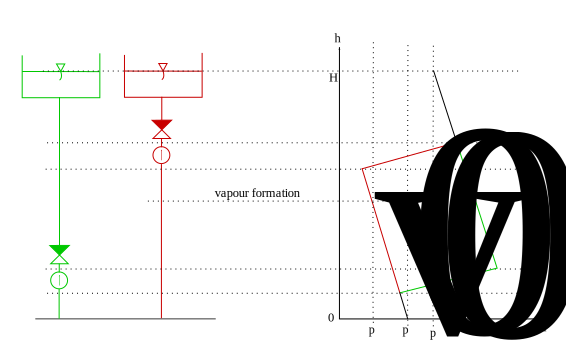
\includegraphics[width=13cm]{figs/cavitation.png}
	\caption{\label{fig:cavitation}Representation of the cavitation.}
	\end{center}
\end{figure}

Two similar arrangement can be seen on left side of Figure \ref{fig:cavitation}. The only difference is the height of the pump, although this cause major deviation in the pressure distribution along the pipe line as it can be observed on the right side of the Figure. In the worst cases the pressure can be below the saturation vapour pressure which means locally the vapour bubbles are appearing. This is called cavitation. The vapour pressure is usually a function of the temperature, e.g.  for water:

\begin{center}
	\begin{tabular}{lcccccc}
	$t[C]$ & 10 & 20 & 40 & 60 & 80 & 100 \\
	$p_v [bar]$ & 0.012 & 0.02 & 0.07 & 0.2 & 0.47 & 1\\
	\end{tabular}
\end{center}

There could be three major consequences of the cavitation:
\begin{itemize}
\item Increased noise among vibration,
\item Drastic decrease in hydraulic performance curve: $H-Q$,
\item Damage of the impeller, see Figure \ref{fig:cavitation_damage}.
\end{itemize}
\begin{figure}[!h]
	\begin{center}
	\centering
	\includegraphics[width=13cm]{figs/cavitation_damage.png}
	\caption{\label{fig:cavitation_damage}Illustration of the cavitation damage in pumps.}
	\end{center}
\end{figure}

\newpage
\subsection{Net Positive Suction Head (NPSH)}

To avoid cavitation it is not sufficient to ensure that the pressure at the suction side is larger than the vapour pressure ($p_s > p_v$). Since  inside the pump there is a complex flow, therefore it is possible to have $p<p_s$ locally where the velocity is large enough. Ensuring the operational work without cavitation the $\mathit{NPSH}$ has to be defined. It is convenient to split the absolute pressure at the pressure side $p_s$ into two parts: $p_v$ vapour pressure plus the part above that, deonted by $\rho g \times NPSH$:
%
\begin{equation}
p_s = p_v + \rho g \times \underbrace{\mathit{NPSH}}_{\text{Net Positive Suction Head}}
\end{equation}
%
this way, the NPSH value gives the net "standby" pressure \emph{above} the vapour pressure that is available before cavitation occurs. 

\begin{figure}[!h]
	\begin{center}
	\centering
	\includegraphics[width=6cm]{figs/NPSH.pdf}
	\caption{\label{fig:NPSH}Representation of the NPSH.}
	\end{center}
\end{figure}

There are two different $\mathit{NPSH}$ values: available ($\mathit{NPSH}_a$) and the required ($\mathit{NPSH}_r$):

\begin{itemize} 
	\item {\bf The available $\mathit{NPSH}_a$} is a {\bf property of the hydraulic system} (geometry, loss coefficients etc. of the pipelines and tanks) and can be evaluated as
\begin{eqnarray}
\mathit{NPSH}_a = \frac{p_t - p_v(T)}{\rho g} - H_s - h'(Q),
\end{eqnarray}
where the $h'(Q)$ represents the frictional losses at the suction-side pipeline (see later in Section \ref{sec:frictionallosses}). 
%
\item {\bf The required $\mathit{NPSH}_r$} value can be found {\bf in the catalogue of the pump}. It is usually depending on the volume flow rate similarly to the head. 
\end{itemize}

The condition for avoiding the cavity is that the available $\mathit{NPSH}$ must be larger than the required $\mathit{NPSH}$, mathematically:
\begin{eqnarray}
\mathit{NPSH}_a > \mathit{NPSH}_r \hspace{1cm} \Longleftrightarrow \hspace{1cm} \text{\textbf{no cavitation}}
\end{eqnarray}

\subsection{Problems}

\vspace{1cm}
\noindent {\bf Problem \thesection.\theprob}\stepcounter{prob}

A pump delivers water from a low-pressure steam boiler as shown in the figure below. Calculate the required geodetic height of the reservoir to avoid cavitation! The pipeline losses are to be taken into account.

\begin{tabular}{cc}
    \begin{minipage}{6cm}
	\begin{center}
	    \resizebox{5cm}{!}{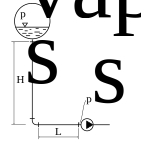
\includegraphics{Problem_solving/figs/PS_NPSH_figure2.png}}\\
	\end{center}
    \end{minipage}
& 

\begin{minipage}{9cm}
\begin{itemize}
\item mass flow rate: $\dot m=27 [kg/s]$, density of the hot water: $\rho=983 [kg/m^3]$
\item pipe: $L=10[m]$, $d=100[mm]$, $\lambda=0.02$ and the sum of loss factors is $\zeta=5$
\item pump: $H[m]=82-4800\,Q^2$, $\mathit{NPSH}[m]=1.6+1360\, Q^2$
\end{itemize}

\emph{Solution:} 

It's easy to calculate that\\
$Q=\dot m/ \rho=0.02747 [m^3/s]$ \\ 
$c_s=Q/A=3.5[m/s]$\\
$H=82-4800 \times 0.02747^2=78.38[m]$\\ 
$\mathit{NPSH}=1.6+1360 \times 0.02747^2=2.626[m]$ 

\end{minipage}
\end{tabular}

\vspace{0.5cm}

Bernoulli's equation between a surface point in the tank and the suction side of the pump reads:

\begin{equation*}
\frac{p_t}{\rho g} + \frac{0^2}{\rho g}+H_s\,=\,\frac{p_s}{\rho g} + \frac{c_s^2}{\rho g}+0+h'_{pipeline}
\end{equation*}

From the suction side of the pump to the impeller we have:

\begin{equation*}
\frac{p_s}{\rho g} + \frac{c_s^2}{2 g}\,=\,\frac{p_{vapour}}{\rho g} + e_s + \mathit{NPSH}
\end{equation*}

(Note that $e_s=0$ as the configuration is horizontal.) Putting the above two equations together, we have

\begin{equation*}
\mathbf{H_s} =-\frac{p_t-p_{vapour}}{\rho g} + h'_{pipe} + \mathit{NPSH}, \quad \text{where} \quad h'_{pipe} = \frac{c_s^2}{2g}\left( \lambda \frac{\mathbf{H_s}+L}{d}+\zeta \right),
\end{equation*}

thus,

\begin{equation*}
H_s =\left( 1-\frac{c_s^2}{2g} \frac{\lambda}{d} \right)^{-1} \left[ \mathit{NPSH} + \frac{c_s^2}{2g} \left( \frac{\lambda L}{d}+\zeta \right) \right]=\dots=8.116[m]
\end{equation*}

Thoma's cavitation coefficient is $\sigma=\mathit{NPSH}/H=0.03355[-]$.

\vspace{1cm}
\noindent {\bf Problem \thesection.\theprob}\stepcounter{prob}

Calculate the required pipe diameter to avoid cavitation, if the pump delivers $Q=30\,\mathrm{dm^3/s}$ water from a closed tank, where the pressure (above the water level) is $p=40\,\mathrm{kPa}$. The equivalent pipe length on the suction side is $5m$, the friction coefficient is $\lambda=0.02$, the suction flange of the pump is $3\,\mathrm{m}$ below the water level. The vapour pressure at the water temperature is $2.8\,\mathrm{kPa}$. The required net positive suction head is $\mathit{NPSH}_r=3.2\,\mathrm{m}$. (The standard pipe diameter series is: DN 40, 50, 65, 80, 90)

\noindent Solution:

\noindent The sketch of the installation is shown in Figure~\ref{fig:NPSH_figure1}

\begin{figure}[ht]
\centering
\includegraphics[width=0.37\textwidth]{Problem_solving/figs/PS_NPSH_figure1.png}
\caption{\label{fig:NPSH_figure1}Installation of the apparatus.}
\end{figure}

\begin{itemize}
\item $\mathit{NPSH}_a=\frac{p_t-p_v}{\rho g}-H_s-h'_s\quad\rightarrow h'_s=\frac{p_t-p_v}{\rho g}-H_s-\mathit{NPSH}_r$
\item $h'_s=\lambda \frac{L_e}{D_s}\frac{c^2_s}{2g}=\lambda \frac{L_e}{D_s}\frac{8Q^2}{D^4_s g \pi^2}$
\item $D_s=0.073m\rightarrow D_s=80\,\mathrm{mm}$
\end{itemize}

\vspace{1cm}
\noindent {\bf Problem \thesection.\theprob}\stepcounter{prob}

Find the required suction side height of the pump that conveys water from an open surface reservoir at $Q=180m^3/h$ flow rate the head is $H=30m$ the required net positive suction head $\mathit{NPSH}_r=5.03m$. The temperature of the water is $T=23^\circ$ the ambient pressure is $p_0=1023mbar$. The hydraulic loss of the suction side pipe can be calculated from $h'_s=652[s^2/m^5]Q^2$ while the vapour pressure $p_v (\mathrm{kPA})=1.704+0.107(t-15)+0.004(t-15)^2$. Find the Thoma cavitation number. (Solution: $H_s=3.481m$, $\sigma=0.1677$)



\clearpage


\chapter{Hydraulic Systems} \label{sec:hydraulic_systems}

\section{Frictional head loss in pipes}\label{sec:frictionallosses}

In hydraulic machinery, instead of pressure $p\,[Pa]$, usually the term \emph{head} is used: $H\,[m]=\frac{p}{\rho g}$.
In real moving fluids, energy is dissipated due to friction, as well as turbulence. Note that as the hydraulic power is $P=\rho gHQ$, but - because of the continuity equation - the flow rate is constant, the energy loss manifests itself in head (pressure) loss.
Head loss is divided into two main categories, "major losses" associated with energy loss per length of pipe, and "minor losses" associated with bends, fittings, valves, etc. The most common equation used to calculate major head losses is the Darcy Weisbach equation:

\beq
h'_f=\lambda\frac{L}{D}\frac{v^2}{2g}=\lambda\frac{L}{D}\frac{8Q^2}{D^4\pi^2 g},
\eeq

where the friction coefficient $\lambda$ (sometimes denoted by $f$) depends on the Reynolds number ($\mathrm{Re}=vD/\nu$, $\nu\,[m^2/s]=\mu/\rho$ being the kinematic viscosity of the fluid) and the relative roughness $e/D$ ($e\,[m]$ being the roughness projections and D  the inner diameter of the pipe). Based on Nikuradse’s experiments, we have different regimes based on the Reynolds number.

\begin{itemize}
\item For laminar flow $\mathrm{Re} < 2300$, we have $\lambda=64$.
\item For transitional flow $2300 < \mathrm{Re} < 4000$, the value of $\lambda$ is uncertain and falls into the range of $0.03\ldots0.08$ for commercial pipes.
\item For turbulent flow in smooth pipes, we have $\frac{1}{\sqrt{\lambda}}=1.95\log(\mathrm{Re}\sqrt{\lambda})-0.55$.
However, this equation need iteration for computing the actual value of $\lambda$. Instead, in the range of $4000 < \mathrm{Re} < 10^5$, the Blasius’s formula is usually used: $\lambda=0.316/\sqrt[4]{Re}$.
\item For turbulent flow in \emph{rough} pipes, Karman-Prandtl equation  may be used: $\frac{1}{\sqrt{\lambda}}=-2\log\left(\frac{e}{3.7D}\right)$. For $Re>4000$, the  Colebrook-White  equation  covers  both the smooth  and  rough regime: $\frac{1}{\sqrt{\lambda}}=-2\log_{10}\left(\frac{2.51}{\mathrm{Re}\sqrt{\lambda}}+\frac{e}{3.7D}\right)$
\end{itemize}

Figure \ref{fig:moody} depicts the Moody diagram, i.e. friction coefficient vs. Reynolds number for different pipe roughness values.

\begin{figure}[ht]
\centering
\includegraphics[width=\textwidth]{figs/moody.png}
\caption{\label{fig:moody}Moody diagram: loss factor $\lambda$ is a straigth pipe.}
\end{figure} 

The loss due to bends, fittings, filters, valves, etc. the minor losses can be taken into account with the help of the loss factor $\zeta$ in the form of

\beq
h'=\zeta\frac{\rho}{2}v^2.
\eeq

In design, minor losses ($\zeta$) are usually estimated from tables using coefficients or a simpler and less accurate reduction of minor losses to equivalent length of pipe (giving the length of a straight pipe with the same head loss), see Table \ref{fig:minor_loss_coeffs} for some examples.

\begin{figure}[ht]
\centering
\includegraphics[width=0.7\textwidth]{figs/abaque-perte-charge.jpg}
\caption{\label{fig:minor_loss_coeffs}Minor loss coefficients.}
\end{figure} 

Another way of characterizing the loss (typically, of valves) is the use of $K_v$ values. The $K_v$ value expresses the amount of flow in a valve (at a given valve position) with a pressure loss of 1 bar. The special situation with a fully open valve determines the $K_{vs}$ value. The amount of flow at a prescribed pressure loss can be calculated using the formula:

\begin{equation}
Q\,\left( m^3/h\right) = K_v \sqrt{\Delta p \left( bar \right)}.
\end{equation}

\section{Head-discharge curves and operating point} \label{sec:head_discharge_curves_and_operating_point}

Let us consider a single pipe with several elbows, fittings, etc. that ends up in a reservoir, see Figure \ref{fig:SimplePumpingSystem}. 

\begin{figure}[ht]
\centering
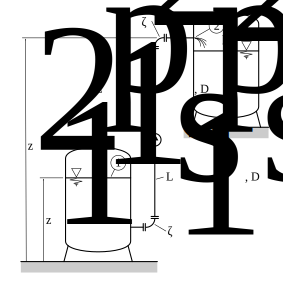
\includegraphics[width=0.45\textwidth]{figs/Hydraulic_system_sample.png}
\includegraphics[width=0.45\textwidth]{figs/performance_curve_simple.png} 
\caption{\label{fig:SimplePumpingSystem}Simple pumping system and its performance curves.}
\end{figure} 

The head $H_{s(ystem)}$ needed to convey $Q$ flow rate covers the pressure difference and the geodetic height difference between the starting and ending point and the losses of the flow: the friction of the pipe, the loss of the elbows, valves, etc., and the discharge loss.

\begin{align}
H_{s(ystem)}&=
\left( \frac{p}{\rho g}+\frac{v^2}{2g}+z\right)_{\text{@ pump outlet}}-
\left( \frac{p}{\rho g}+\frac{v^2}{2g}+z\right)_{\text{@ pump inlet}}\nonumber\\
&=\left(\frac{p_2}{\rho g}+\frac{v_2^2}{2g}+z+h'_{\text{after the pump}}\right)-
\left(\frac{p_1}{\rho g}+z_1+h'_{\text{before the pump}}\right)\nonumber\\
&=\frac{p_2-p_1}{\rho g}+\left(z_2-z_1\right)
+\left(\underbrace{\sum\zeta+\sum\lambda\frac{L}{D}}_{\text{frictional loss of the pipeline}}+1\right)\frac{v^2}{2g}\nonumber\\
&=\underbrace{\frac{p_2-p_1}{\rho g}+\left(z_2-z_1\right)}_{H_{static}}
+\underbrace{\left(\sum\zeta+\sum\lambda\frac{L}{D}+1\right)\frac{1}{2gA^2}}_{B}Q^2\nonumber\\
&=H_{stat}+BQ^2
\end{align}

We see that the total head of the system consists of two parts: $H_{stat}$, that does \emph{not} depend on the actual flow rate and $BQ^2$, which varies with the flow rate. Figure \ref{fig:SimplePumpingSystem} depicts the pump head curve, the system head curve and the intersection, that is, the actual flow rate and head that the pump conveys through the system. 



\section{Problems}

\noindent {\bf Problem \thesection.\theprob}\stepcounter{prob}

Consider the flow of water in a pipe of $L=100$m, $D=100$mm and the pipe roughness is $e=4$mm. The flow rate is $Q=36.7\,\mathrm{m^3/h}$. Find the pressure drop.

\noindent Solution:
%
\begin{itemize}
\item The flow velocity $v=\frac{36.7}{3600} / \frac{0.1^2\pi}{4}=1.3$m/s.
\item The Reynolds number is $Re=vD/\nu=1.3\times 10^{5}$ (the kinematic viscosity of water is $\nu=10^{-6}\mathrm{m^2/s}$).
\item If the pipe were hydraulically smooth, the friction coefficient would be $\lambda=\frac{0.316}{\sqrt[4]{Re}}=0.0166$.
\item We use the Colebrook-White equation iteratively, starting from $\lambda_0=0.0166$:
	\begin{itemize}
		\item Step 1: $\frac{1}{\sqrt{\lambda_1}}=-2\log_{10}\left(\frac{2.51}{\mathrm{Re}\sqrt{\lambda_0}}+\frac{e}{3.7D}\right)=-2\log_{10}\left(\frac{2.51}{\mathrm{1.3\times 10^{5}}\sqrt{0.0166}}+\frac{4}{3.7\times100}\right)=3.9203$, thus $\lambda_1=0.065$.
		%
		\item Step 2:$\frac{1}{\sqrt{\lambda_1}}=-2\log_{10}\left(\frac{2.51}{\mathrm{Re}\sqrt{\lambda_1}}+\frac{e}{3.7D}\right)=-2\log_{10}\left(\frac{2.51}{\mathrm{1.3\times 10^{5}}\sqrt{0.065}}+\frac{4}{3.7\times100}\right)=3.9262$, thus $\lambda_1=0.0649$. This is reasonably close to $\lambda_1$, hence we stop the iteration.
	\end{itemize}
\item Finally, the pressure drop is $\Delta_p'=\lambda \frac{L}{D}\frac{\rho}{2}v^2=0.0649\frac{100}{0.2}\frac{1000}{2}1.3^2=54.84\mathrm{kPa}=0.548\mathrm{bar}$.
\end{itemize}


\noindent {\bf Problem \thesection.\theprob}\stepcounter{prob}

Calculate the head loss of the pipe depicted in the figure below as a function of the volume flow rate! Parameters: $\zeta_A=1.5$, $\zeta_{B,D}=0.26$, $\zeta_C=0.35$, $\zeta_F=0.36$, $\lambda=0.0155$, $D_s=D_p=D=0.6[m]$ and $Q=0.4[m^3/s]$. 
% 
\begin{figure}[ht]
\begin{center}
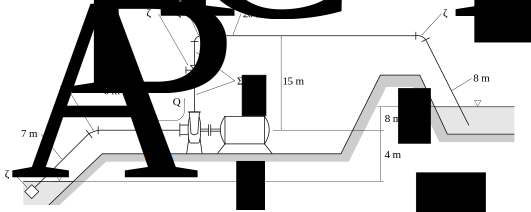
\includegraphics{Problem_solving/figs/PS_HydraulicSystems1.png}
\end{center}
\end{figure}
%
\noindent Solution:
%
\begin{itemize}
\item Static (geodetic) head + dynamic (friction) losses of the pipe: $H_{pipe}=H_{stat}+H_{friction}$
\item Volume flow rate: $Q=c_{s(uction)}A_{pipe,suction}=c_{p(ressure)}A_{pipe,pressure}=c A_{pipe}$
\item The 'extra' $1$ in the pressure side ($...\zeta_D+1$) represents the outflow losses.
\item $H_{stat}=8+4=12[m]$, $L_s=7+6=14[m]$, $L_p=12+20+8=40[m]$
\end{itemize}
%
\begin{alignat*}{1}
H_{pipe}&=H_{stat}+KQ^2= H_{stat}+\left[ \left( \lambda\frac{L_s}{D_s}+\zeta_A+\zeta_B\right)\frac{c_s^2}{2g}\,+\,\left( \lambda\frac{\sum L_p}{D_p}+\zeta_F+\zeta_C+\zeta_D+1\right)\frac{c_p^2}{2g}\right]=\\
%	&=H_{stat}+Q^2\frac{8}{g \pi^2}\left[ \left( \lambda\frac{L_s}{D_s}+\zeta_A+\zeta_B\right)\frac{1}{D_s^4}\,+\,\left( \lambda\frac{\sum L_p}{D_p}+\zeta_F+\zeta_C+\zeta_D+1\right)\frac{1}{D_p^4}\right]=...\\
	&=12[m]+3.25[s^2/m^5] \times Q^2 [m^3/s]^2
\end{alignat*}

%%%%%%%%%%%%%%%%%%%%%%%%%%%%%%%%%%%%%%%%%%%%%%%%%%%%%%%%%%%%%%%%%%%%%%%%%%%%%

\vspace{1cm}
\noindent {\bf Problem \thesection.\theprob}\stepcounter{prob}

The artificial fountain Beneath the St. Gellert  is fed by two pipelines of $30m$ length. The height distance between the pump and the fountain is $22m$. The diameter of the pipes is $D_1=100mm$ and $D_2=70mm$, the friction coefficient of the straight segments is $\lambda=0.02$ and the friction coefficient of the other segments (bends, etc.) is $\zeta=0.5$. Assuming that the flow velocity in the second pipe is $1.5m/s$, calculate the the required head. Calculate the flow velocity in the second pipe and the overall flow rate of the common pump feeding the two pipes.Assuming $65\%$ overall (pump+motor) efficiency, calculate the energy demand for 100 days and the cost of the operation if the energy tariff is $32 HUF/kWh$. (Solution: Without the bypass line: $H=22.826m[$], $Q=0.01678[m^3/s]$, $P=5.78[kW]$ and $Cost=443691HUF$.)

%%%%%%%%%%%%%%%%%%%%%%%%%%%%%%%%%%%%%%%%%%%%%%%%%%%%%%%%%%%%%%%%%%%%%%%%%%%%%%%%%%%
\newpage

\vspace{1cm}
\begin{tcolorbox}
\noindent {\bf Problem \thesection.\theprob}\stepcounter{prob}

A pump delivers $Q=1200[dm^3/min]$ water from an open-surface well, whose water level is $25[m]$ below the default level. The pressure side ends $5[m]$ above the default level and the water flows into an open-surface swimming pool. The diameter of the pipe on the suction side is $D_s=120[mm]$ and $D_p=100[mm]$ on the pressure side. The loss coefficients are $\zeta_s=3.6$ and $\zeta_p=14$ (without the outflow losses). Calculate the required pump head! (Solution: $H_{p,req.}=35.7[m]$) Draw a sketch of the system! (Figure\ref{gen_hs})
\vspace{0.2cm}

Solution:
\vspace{0.2cm}

The points which marked with I and II indicates the beginning and the end of the pump. The whole system is between $1' - 2$ points. The end of the draft tube shall be deep under the fluid surface to avoid the air intake. But in this problem we neglect the x value (the height between the end of the tube and the fluid surface).

Bernoulli equation between $1'$ and $I$: ${e_1}'=e_{I.}+{h_s}'$ it follows ${e_{I.}}'=e_{1}'+{h_s}'$

Bernoulli equation between II and $2$: $e_{II.}=e_2+{h_p}'$, in these formulas, e denotes the “Bernoulli sum” of meter units.The volume flow rate is based on the description of the problem $Q = 1200dm^3/min = 0,02m^3/s$. The head losses for the intake and the delivery ports:
\begin{equation*}
{h_s}'=\zeta_s \frac{{v_s}^2}{2g}=\zeta_s \frac{1}{2g}\frac{Q^2}{{A_s}^2}=3.6\times\frac{1}{2\times 9.81}\times\frac{0.02^2}{\left(0.12^2\times\frac{\pi}{4}\right)}^2=3.6\times\frac{1}{2\times 9.81}\times\frac{0.02^2}{0.01131^2}=0.5738m	
\end{equation*}
\begin{equation*}
{h_p}'=\zeta_p \frac{{v_p}^2}{2g}=\zeta_p \frac{1}{2g}\frac{Q^2}{{A_p}^2}=14\times\frac{1}{2\times 9.81}\times\frac{0.02^2}{\left(0.1^2\times\frac{\pi}{4}\right)}^2=14\times\frac{1}{2\times 9.81}\times\frac{0.02^2}{0.007854^2}=4.627m	
\end{equation*}
\begin{equation*}
v_2=\frac{Q}{A_p}=\frac{0.02}{0.01131}=2.546 m/s	
\end{equation*}
(the specific kinetic energy of the water flow leaving at this speed is lost in the swimming pool (2), its name is the discharge loss,$\frac{v_2^2}{2g}$)
\begin{equation*}
H_{st}=z_2-z_1=25-(-5)=30m \text{  (static head)}	
\end{equation*}
The head of the system (static head+ discharge loss):
\begin{equation*}
H_{system}=H_st+\frac{{v_2}^2}{2g}=30+\frac{2.546^2}{2\times 9.81}=30.33m
\end{equation*}
The head of the pump:
\begin{equation*}
	H_{pump}=e_{II.}-e_{I.}=(e_2+{h_p}')-({e_1}'-{h_s}')=e_2-{e_1}'+{h_p}'+{h_s}'=
\end{equation*}
\begin{equation*}
=\left(\frac{p_2}{\rho g}+\frac{{v_2}^2}{2g}+z_2\right)-\left(\frac{p_{1'}}{\rho g}+\frac{{v_{1'}}^2}{2g}+z_{1'}\right)+{h_p}'+{h_s}'
\end{equation*}
at the surface of the fluid $p_1 = p_0$ (atmospheric pressure), and $v_1 = 0$, because of the relatively large surface of the well, this equation is substituted in the 2nd parentheses of the above equation.
Using that $p_2 = p_0$ is also true:
\begin{equation*}
	H_{sz}=\left(\frac{p_2}{\rho g}+\frac{{v_2}^2}{2g}+z_2\right)-\left(\frac{p_1}{\rho g}+\frac{{v_{1}}^2}{2g}+z_1 \right)+{h_n}'+{h_s}'=\left(\frac{p_0}{\rho g}+\frac{{v_2}^2}{2g}+z_2\right)-\left(\frac{p_{0}}{\rho g}+\frac{0}{2g}+z_1\right)+{h_n}'+{h_s}' 
	\end{equation*}
\begin{equation*}
H_{sz}=\frac{{v_2}^2}{2g}+z_2-z_1+{h_n}'+{h_s}'=35.53m
\end{equation*}
But we can also write that the head of the pump covers the head of the system as well as the losses: $H_{sz}=H_{system}+{h_n}'+{h_s}'=30.33m+4.627m+0.5738m=35.53m$
\end{tcolorbox}

\begin{figure}[ht]
\begin{center}
\includegraphics[scale=0.75]{figs/problem_3p3p34_hyd_sys_fig.png}
\caption{\label{gen_hs}Hydraulic system}
\end{center}
\end{figure}
\vspace{1cm}
\noindent {\bf Problem \thesection.\theprob}\stepcounter{prob}

The submergible pump shown in the picture below delivers $Q = 30 l/s$ water into the basin. The pipe collecting the water of five equal pumps has a diameter $D$. The inner diameter of the pressure tube connecting the pump with the collecting pipe is $d$. Find the Bernoulli enthalpy difference between the two ends of the system, and the pump head! Further data are: $D = 400 mm$, $\lambda_D = 0.018$, $d = 160 mm$, $\lambda_d = 0.021$, $\zeta_{filter} = 3$ , $\zeta_{nrv}=0.25$, $\zeta_{bd} = 0.35$, $\zeta_{2bd} = 0.5$, $\zeta_{bD} = 0.22$. (Solution: $\Delta e_{system}=11.07m$, $H_{pump}=12.80m$)
% 
\begin{figure}[ht]
\begin{center}
\includegraphics{Problem_solving/figs/PS_HydraulicSystems_Submergible.png}
\end{center}
\end{figure}

%%%%%%%%%%%%%%%%%%%%%%%%%%%%%%%%%%%%%%%%%%%%%%%%%%%%%%%%%%%%%%%%%%%%%%%%%%%%%

\vspace{1cm}
\noindent {\bf Problem \thesection.\theprob}\stepcounter{prob}

The head of a 4 stage pump is $68~\mathrm{m}$, the speed of revolution is $1450~\frac{\mathrm{1}}{\mathrm{min}}$. This pump conveys water through a horizontal pipe with diameter $D=120~\mathrm{mm}$. The volumetric flow rate is $0.03~\frac{\mathrm{m^3}}{\mathrm{s}}$. The friction coefficient of the pipe is $\lambda=0.025$. Find the length of the pipe, after which an additional pump needs to be built in the system, if the requirement is that the pressure in the pipe cannot be lower than it is at the suction side! Calculate the same distance in the case when the pipe diameter is $D=160~\mathrm{mm}$! When fewer pumps are in the system, the cost of the investment is obviously lower. Calculate the approximation of the investment cost as a function of the pipe diameter! (hint: the investment cost has two parts: one which is proportional to the pipe length per pump, and another which is proportional to the material cost (thickness of the pipe)). (Solution: $L_1=910.5~\mathrm{m}$, $L_2 = 3835~\mathrm{m}$, $cost=\frac{k_1}{D^5} + k_2 D^2$.)

%%%%%%%%%%%%%%%%%%%%%%%%%%%%%%%%%%%%%%%%%%%%%%%%%%%%%%%%%%%%%%%%%%%%%%%%%%%%%

\vspace{1cm}
\noindent {\bf Problem \thesection.\theprob}\stepcounter{prob}

Find the operation point of a pump which operates a fountain in a lake! The diameter of the pipe at the outlet is $30~\mathrm{mm}$, and the water jet has to reach a height of $20~\mathrm{m}$. The elevation of the jet can be calculated from Newton's law and the gravitational acceleration. However, due to the breaking up of the jet into drops, the jet reaches only $80~\%$ of the theoretical height. At the suction side of the pump, there is a filter, which is characterized by the loss coefficient $\zeta_s=0.7$. At the pressure side, the length of the pipe is $L=1~\mathrm{m}$, the friction coefficient is $\lambda=0.02$, and there are two elbows with loss coefficient $\zeta_e=0.2$ for each of them. The diameter of the pipe at the suction and pressure side is $D=80~\mathrm{mm}$.  Find the specific speed of the pump, if the speed of rotation is $n=1470~\frac{1}{\mathrm{min}}$ and the pump has two stages! Calculate the height of the water jet, if the speed of rotation drops to $n=970~\frac{1}{\mathrm{min}}$! (Solution: $Q=0.01565~\frac{\mathrm{m^3}}{\mathrm{s}}$, $H=25.668~\mathrm{m}$, $n_q=27.13$, $h_{fountain,n=970}=8.71~\mathrm{m}$.)

%%%%%%%%%%%%%%%%%%%%%%%%%%%%%%%%%%%%%%%%%%%%%%%%%%%%%%%%%%%%%%%%%%%%%%%%%%%%%

\vspace{1cm}
\noindent {\bf Problem \thesection.\theprob}\stepcounter{prob}

In a concrete pipe with diameter $D_o = 2800~\mathrm{mm}$ ($\lambda_o=0.03$), there is a smaller pipe with diameter $D_i=1000~\mathrm{mm}$ ($\lambda_i=0.02$). The inner pipe is in the center of the outer pipe. The length of both pipes is $L=540~\mathrm{m}$. The height difference is $\Delta h=3~\mathrm{m}$, and this geodetic head drives the flow. Find the volumetric flow rate
\begin{enumerate}
\item when there is no smaller pipe in the larger pipe and
\item when the smaller pipe is in the larger one!
\end{enumerate}
The friction coefficients should be weighted with the wetted area! (Solution: $Q_1=70713~\frac{\mathrm{m^3}}{\mathrm{h}}$, $Q_2=51830~\frac{\mathrm{m^3}}{\mathrm{h}}$.)


\clearpage


\chapter{Fans} \label{chpt:fans}

\section{Problems}

\noindent {\bf Problem \thesection.\theprob}\stepcounter{prob}

A fan conveys air that's density is $1.2~\frac{\mathrm{kg}}{\mathrm{m^3}}$. 
%The pressure at the suction side is approximately the atmospheric pressure, at the pressure side the pressure is $200~\mathrm{Pa}$ higher. 
The pressure difference between the pressure and suction sides is $200~\mathrm{Pa}$. 
The volumetric flow rate is $Q=0.4~\frac{\mathrm{m^3}}{\mathrm{s}}$, the diameter of the duct at the suction side is $D_1=200~\mathrm{mm}$, and the duct diameter at the pressure side is $D_2=250~\mathrm{mm}$. Find the static and total pressure difference created by the fan! Find the useful power of the fan! (Solution: $\Delta p_{stat} = 102.8~\mathrm{Pa}$, $\Delta p_{tot} = 142.6~\mathrm{Pa}$, $P_u = 57.03~\mathrm{W}$). 


%%%%%%%%%%%%%%%%%%%%%%%%%%%%%%%%%%%%%%%%%%%%%%%%%%%%%%%%%%%%%%%%%%%%

\vspace{1cm}
\noindent {\bf Problem \thesection.\theprob}\stepcounter{prob}

The mean diameter of an axial fan is $D_m = 500~\mathrm{mm}$, the speed of rotation is $n=1450~\frac{1}{\mathrm{min}}$. The inlet blade angle is $\beta_1 = 9.1^\circ$, the blade angle at the outlet is $\beta_2 = 12.3^\circ$, and the axial velocity is $c_{ax} = 6.2~\frac{\mathrm{m}}{\mathrm{s}}$. Find the ideal total pressure difference created by the fan using Euler's turbine equation! What is the actual total pressure difference, if the hydraulic efficiency is $\eta_h=80\%$? Find the static pressure difference! (Solution: $\Delta p_{tot,id} = 433.9~\mathrm{Pa}$, $\Delta p_{tot} = 347.1~\mathrm{Pa}$, $\Delta p_{stat} = 324.1~\mathrm{Pa}$).


%%%%%%%%%%%%%%%%%%%%%%%%%%%%%%%%%%%%%%%%%%%%%%%%%%%%%%%%%%%%%%%%%%%%%%

\vspace{1cm}
\begin{tcolorbox}
\noindent {\bf Problem \thesection.\theprob}\stepcounter{prob}

How does the pressure difference change for the axial CPU fan in Problem 2.2.12, if we install guiding vanes after the fan that eliminate the circumferential velocity component of the flow at the exit? 

(Note that this problem is only a demonstration of the calculation. In reality, CPU fans are never equipped with guiding vanes, because their efficiency is not the most important parameter. A more important parameter of CPU fans is noise.)
%Find the inlet blade angle of the guiding vanes!

Solution:
The calculation of problem 2.2.12:
\begin{itemize}
\item $A_{ring}=\frac{\left(D_o^2-D_i^2\right)\pi}{4}=0.00137\,\mathrm{m^2}$
\item $D_{mean}=\frac{D_o+D_i}{2}=0.03425\,\mathrm{m}$
\item $u_{mean}=u_1=u_2=D_{mean}\pi n=4.913\,\mathrm{\frac{m}{s}}$
\item $c_{ax}=c_{1,ax}=c_{2,ax}=u \tan\beta_1=1.788\,\mathrm{\frac{m}{s}}$
\item $q=\eta_{vol}A_{ring}c_{ax}=0.00184\,\mathrm{\frac{m^3}{s}}$
\item $w_{2u}=\frac{c_{ax}}{\tan\beta_2}=2.131\,\mathrm{\frac{m}{s}}$
\item $\Delta c_u=u-w_{2u}=2.782\,\mathrm{\frac{m}{s}}$
\item $\Delta p_{total,ideal}=\rho u\Delta c_u=17.1\,\mathrm{Pa}$
\item $\Delta p_{total}=\eta_h \Delta p_{total,ideal}=14.5\,\mathrm{Pa}$
\end{itemize}

The guiding vane eliminates the circumferential velocity component, while the axial velocity remains the same because the continuity equation needs to be satisfied. Using all this information, we can use Bernoulli's equation between the inlet and the outlet of the guiding vane:
\begin{align*}
& p_2 + \frac{\rho}{2}c_2^2 = p_2 + \frac{\rho}{2} (c_{ax}^2 + c_{2u}^2) = p_3 + c_3^2 = p_3 + c_{ax}^2. 
\end{align*} 
In the equation above, the index 2 denotes the outlet of the impeller blade, which is the same as the inlet of the guiding vane; the index 3 denotes the outlet of the guiding vane. From this equation, the pressure difference $p_3 - p_2$ can be calculated:
\begin{align*}
& dp = p_3 - p_2 = \frac{\rho}{2}c_{2u}^2 = \frac{1.25}{2}\cdot 2.782^2 = 4.838~\mathrm{Pa}. \\
& \Delta p_{total,vane} = \Delta p_{total} + dp = 19.36~\mathrm{Pa}.
\end{align*}
\end{tcolorbox}
%The inlet angle of the guiding vane 


%%%%%%%%%%%%%%%%%%%%%%%%%%%%%%%%%%%%%%%%%%%%%%%%%%%%%%%%%%%%%%%%%%%%%%

\vspace{1cm}
\noindent {\bf Problem \thesection.\theprob}\stepcounter{prob}

The acoustic power in a bus station is $P_{ac} = 4.3~\mathrm{mW}$. Find the acoustic power level! How does the power level change, if the acoustic power changes to $P_{ac,1} = 2P_{ac}$, $P_{ac,2} = 5P_{ac}$, $P_{ac,3} = 8P_{ac}$, $P_{ac,4} = 0.1P_{ac}$? (Solution: $L_w = 96.33~\mathrm{dB},~L_{w,1} = 99.35~\mathrm{dB},~L_{w,2} = 103.32~\mathrm{dB},~L_{w,3} = 105.37~\mathrm{dB},~L_{w,4} = 86.33~\mathrm{dB}$).


%%%%%%%%%%%%%%%%%%%%%%%%%%%%%%%%%%%%%%%%%%%%%%%%%%%%%%%%%%%%%%%%%%%%%%
% feladatgyujtemeny 11.2
\vspace{1cm}
\noindent {\bf Problem \thesection.\theprob}\stepcounter{prob}

An axial fan, which has no guiding vanes, conveys air at volumetric flow rate $Q=2~\frac{\mathrm{m^3}}{\mathrm{s}}$, density $\rho=1.2~\frac{\mathrm{kg}}{\mathrm{m^3}}$, while the static pressure difference is $p_{st} = 120~\mathrm{Pa}$. Find the total pressure difference, if the  diameter of the pipe is $D=450~\mathrm{mm}$! Find the useful power! Calculate the efficiency, if the power of the motor is $P_{in} = 500~\mathrm{W}$! The speed of the fan is $n=960~\frac{\mathrm{1}}{\mathrm{min}}$. Find the sound power level of the fan, using the formula: $L_W = 97 + 10\cdot \log_{10}(Q\cdot \Delta p_{tot} \cdot (\frac{1}{\eta}-1)) + 32\cdot \log_{10}(\frac{u_2}{a})(\mathrm{dB})$. The sonic speed is $a=340~\frac{\mathrm{m}}{\mathrm{s}}$. Draw the velocity triangles at the tip of the fan! In the calculations, you can ignore the fact that the hub locally increases the velocity, and the leakage losses and the loss due to the circumferential velocity component can be also ignored.

(Solution: $\Delta p_{tot} = 215~\mathrm{Pa}$, $P_u = 430~\mathrm{W}$, $\eta = 0.86$, $L_W = 77.8~\mathrm{dB}$, $u = 22.62~\frac{\mathrm{m}}{\mathrm{s}}$, $c_{ax} = 12.58~\frac{\mathrm{m}}{\mathrm{s}}$, $\Delta c_{u} = 7.92~\frac{\mathrm{m}}{\mathrm{s}}$)

%%%%%%%%%%%%%%%%%%%%%%%%%%%%%%%%%%%%%%%%%%%%%%%%%%%%%%%%%%%%%%%%%%%%%%
% feladatgyujtemeny 11.3
\vspace{1cm}
\noindent {\bf Problem \thesection.\theprob}\stepcounter{prob}

The dryers in a forage dryer facility are spatially separated. The air to the dryers is conveyed by two identical centrifugal fans, that's performance curve is $\Delta p_{fan,tot} = 1200 - 300\Big(\frac{\mathrm{Pa}\cdot\mathrm{s^2}}{\mathrm{m^6}} \Big)Q^2$. The characteristic curve of the dyers is $\Delta p_{dryer,tot} = 900\Big(\frac{\mathrm{Pa}\cdot\mathrm{s^2}}{\mathrm{m^6}}\Big) Q^2$. Find the volumetric flow rate, is one dryer is connected one fan! Find the operating point, if two in parallel connected dryers are supplied by (i) two fans in series connection or (ii) two fans in parellel connection!

(Solution:$Q_1 = 1~\frac{\mathrm{m^3}}{\mathrm{s}}$, $Q_{series} = 1.706~\frac{\mathrm{m^3}}{\mathrm{s}}$, $Q_{parallel} = 2~\frac{\mathrm{m^3}}{\mathrm{s}}$)

%%%%%%%%%%%%%%%%%%%%%%%%%%%%%%%%%%%%%%%%%%%%%%%%%%%%%%%%%%%%%%%%%%%%%%
% feladatgyujtemeny 11.4
\vspace{1cm}
\begin{tcolorbox}
\noindent {\bf Problem \thesection.\theprob}\stepcounter{prob}

The "snow cannon" of a ski slope is an axial fan, that accelerates air that's density is $\rho = 1.32~\frac{\mathrm{kg}}{\mathrm{m^3}}$ to velocity $c=30~\frac{\mathrm{m}}{\mathrm{s}}$. Following the impellers, a mass flow rate of $\dot{m}=4~\frac{\mathrm{kg}}{\mathrm{s}}$ water is sprayed into the air, and the water is accelerated to the speed of the air. Find the impulse change of the water! Find the pressure required to accelerate the water, if the cross-section of the of the fan after the impellers is $A=0.2~\mathrm{m^2}$. Find the static and total pressure difference, if the air-water mixture exits directly to the open after the fan! Sketch the static and total pressure along a streamline!

\begin{itemize}
%
\item The watr needs to be accelerated from 0 to 30 m/s; the impulsa change is $\Delta I = \dot{m}_w c=120~\frac{\mathrm{kg m}}{\mathrm{s^2}}$.
%
\item This impulse change is coeverd by the pressure difference of the pump: $A\Delta p=\Delta I$, hence $\Delta p=600$Pa.
%
\item After the water injection, the average density of the water-air mixture is $\rho_m=\frac{Q_{air}\rho_{air}+Q_w\rho_w}{Q_{air}+Q_{water}}=\frac{30 m/s\times 0.2m^2+4kg/s}{6m^3/s+0.004 m^3/s}$, which is the weighted average of the densities, wieghted by the mass flow rates. We also have $Q_{air}=30 m/s\times 0.2m^2=6m^3/s$ and $Q_w=4kg/s/1000 kg/m^3=0.004m^3/s$.
%
 \item The dynamic pressure of the mixture is $894~\mathrm{Pa}$, see Figure \ref{fig:snow_cannon}.
\end{itemize}
\end{tcolorbox}

\begin{figure}[!ht]
\centering
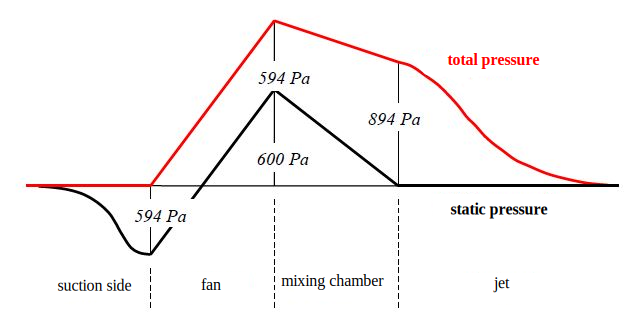
\includegraphics[width = 0.5\textwidth]{Problem_solving/figs/snow-cannon.png}
\caption{\label{fig:snow_cannon} Pressure distribution in the "snow cannon".}
\end{figure}

%%%%%%%%%%%%%%%%%%%%%%%%%%%%%%%%%%%%%%%%%%%%%%%%%%%%%%%%%%%%%%%%%%%%%%
% feladatgyujtemeny 11.7
\vspace{1cm}
\noindent {\bf Problem \thesection.\theprob}\stepcounter{prob}

\begin{wrapfigure}{R}{0.4\textwidth}
\includegraphics[width=0.4\textwidth]{Problem_solving/figs/car-engine-cooler.JPG}
\end{wrapfigure}

The nominal area of the radiator of a car engine cooler is $A=0.12~\mathrm{m^2}$, and it's loss coefficient is $\zeta = 1.2$. The performance curve of the cooling fan is $\Delta p_{tot} = 147 (\mathrm{Pa}) - 300\cdot \Big(\frac{\mathrm{Pa}\cdot\mathrm{s^2}}{\mathrm{m^6}} \Big)(Q-0.3)^2$. The fan conveys the hot air with density $\rho=1.1~\frac{\mathrm{kg}}{\mathrm{m^3}}$ from it's suction side through the radiator. The outer diameter of the fan is $D_o = 310~\mathrm{mm}$, and the hub diameter is $D_i = 140~\mathrm{mm}$. The air, after it leaves the fan, arrives to the engine space and slows down, while it's pressure reaches the pressure of the ambient air. 

Write down Bernoulli's equation for a stading car, between the far-field point in front of the radiator and the suctions side of the fan, and an other Bernoulli-equation between the pressure side of the fan and the engine space. Using these equations and the performance curve of the fan, find the volumetric flow rate! Sketch the static, dynamic and total pressure along a streamline, between the far field point - suction side and the pressure-side - engine space!

(Solution: $Q=0.7036~\frac{\mathrm{m^3}}{\mathrm{s}}$)

%%%%%%%%%%%%%%%%%%%%%%%%%%%%%%%%%%%%%%%%%%%%%%%%%%%%%%%%%%%%%%%%%%%%%%
% feladatgyujtemeny 11.5
\vspace{1cm}
\noindent {\bf Problem \thesection.\theprob}\stepcounter{prob}

Find the relative pressure needed to support an inflatable tennis court tent, id the are if the tent is $22\times 40~\mathrm{m^2}$, and the mass of the tent is $m=3000~\mathrm{kg}$. How long does it take to set up such an inflatable tent, if the performance curve of the fan we use is $\Delta p_{tot} = 70~\mathrm{Pa} - 42\cdot \Big(\frac{\mathrm{Pa}\cdot\mathrm{s^2}}{\mathrm{m^6}} \Big)Q^2$ and the average height of the tent is 5 m? The density of the air is $\rho = 1.3~\frac{\mathrm{kg}}{\mathrm{m^3}}$, the cross-section of the fan at the pressure side is $A=0.2~\mathrm{m^2}$, and the fan conveys the air between two open spaces! Find the stationary leakage flow rate from the tent, if the area of the holes on the tent (which ensure a cross flow through the tent to provide fresh air) is $A_l = 0.05~\mathrm{m^2}$! Find the relative pressure in the tent!

(Solution: $\Delta p = 33.4~\mathrm{Pa}$, $t=1.54~\mathrm{h}$, $v=0.469~\frac{\mathrm{m^3}}{\mathrm{s}}$, $\Delta p_{stat} = 57~\mathrm{Pa}$)





\clearpage

\chapter{Control}

\section{Adjusting a desired operating point}

\subsection{Terminology}


Consider the problem of setting a desired $Q_d$ flow rate at the pipeline system with head-discharge problem of $H_s$. If we simply connect a pump to the system, the provided flow rate will not be the desired one but the the flow rate corresponding to the intersection of the pump and pipeline curve. By controlling either the pump or the system (via valves), we can achieve the desired flow rate. However, it is typical that either the $Q_p$ flow rate of the pump or the $H_p$ head of the pump is not the same as that of the pipeline system

When making decisions on pump or fan control, we use two following important quantities.

\begin{description}
\item[Control efficiency.] This quantity is the ratio of the useful power and the input power, that is
\begin{equation}
\eta=\frac{P_{useful}}{P_{input}}=\frac{Q_d \rho g H_s(Q_d)}{Q_p \rho g H_p(Q_p)}
\end{equation}
%
\item[Specific energy consumption.] This quantity is the ratio of the input power and the flow rate, that is
\begin{equation}
\text{SEC}=\frac{P_{input}}{Q_d}=\frac{P_{input}}{V/t}=\frac{\text{energy consumed}}{\text{volume of fluid}},
\end{equation}
that is, the energy consumption of conveying 1 $m^3$ of fluid in the system.
\end{description}

We shall analyse three ways of control:

\begin{enumerate}
\item Control via a valve connected in series.
\item Control via a valve connected in parallel, i.e. by-pass valve.
\item Control via a changing the pump revolution number.
\end{enumerate}

\clearpage

\subsection{Valve in series}


%\begin{figure}
\begin{wrapfigure}{r}{0.6\textwidth}
\includegraphics[width=0.6\textwidth]{figs/series_connection.pdf}
\caption{Control via a valve connected in series.}
\end{wrapfigure}
%\end{figure}

In the case of series valve control, we add a throttle valve at the pressure side of the pump. (And never at the suction side, due to the danger of cavitation!) As the three element are now connected in series, the flow rate is common, while the pressure will change. 

The efficiency is $\eta=\frac{Q_d \rho g H_s}{P_{pump}}$, where $P_{pump}=H_p\rho g Q_d /\eta_{pump}(Q_d)$, hence we have $\eta=\eta_{pump}(Q_d)H_s/H_p$. That is, the ratio of the system head and the pump head, multiplied by the efficiency of the pump at the operating point. The specific energy consumption is SEC$=\rho g H_p(Q_d)/\eta_{pump}(Q_d)$. 

This type of control introduces new head loss at the pressure side, resulting in a higher overall pipeline loss, which than reduces the head of the pump. The power lost on the throttle valve is $P'_v=Q_d \rho g H'_v$.

\subsection{Bypass valve (parallel)}


%\begin{figure}
\begin{wrapfigure}{r}{0.6\textwidth}
\includegraphics[width=0.6\textwidth]{figs/parallel_connection.pdf}
\caption{Control via a valve connected in series.}
\end{wrapfigure}
%\end{figure}

In the case of a bypass valve, we add a throttle valve parallel with the pump to allow backflow of unnecessary fluid into the suction-side reservoir.  As the three element are now connected in parallel, the flow rate adds up, while the pressure difference is the same. 

The efficiency is $\eta=\frac{Q_d \rho g H_s}{P_{pump}}$, where $P_{pump}=H_s\rho g Q_p/\eta_{pump}(Q_p)$, hence we have $\eta=\eta_{pump}(Q_p)Q_s/Q_p$. That is, the ratio of the desired flow rate and the pump flow rate, multiplied by the efficiency of the pump at the pump operating point. The specific energy consumption is SEC$=\rho g H_p(Q_p)Q_p/Q_d /\eta_{pump}(Q_p)$.

This type of control does not introduce new head loss, but allows a portion of the (too large) pump flow rate back to the reservoir. The power lost on the throttle valve is $P'_v=Q_v \rho g H_s$.

\section{Pump revolution number control}

A common way of setting pump flow rate is to vary the revolution number. Intuitively, decreasing the pump revolution number will result in lower flow rate, while increasing it will result in higher flow rate.

Combining the affinity laws $Q_2/Q_1=n_2/n_1$ and $H_2/H_1=n_2^2/n_1^2$ give $H_2=\left( H_1/Q_1^2\right)Q_2^2:=a\,Q_2^2$. This simply means that while changing the revolution number, the operating point moves along an \emph{central parabola} $a Q^2$ that starts from the origin and passes through the original point $\left( Q_1,H_1\right)$. \emph{The affinity law can be used only between point lying on the same central parabola.}

See the first problem in the next section for a worked example.

\subsection{Problems}

\noindent {\bf Problem \thesection.\theprob}\stepcounter{prob}

A pump running at $1470 [rpm]$ with $H_{pump}=45-2781 Q^2$ head delivers water into a pipeline with $H_{pipe}=20+1125Q^2$. Calculate the required revolution number for the reduced flow rate $Q'=0.05 [m^3/s]$. 

\vspace{0.5cm}
\begin{tabular}{cc}
    \begin{minipage}{9cm}
	\begin{center}
	    \resizebox{9cm}{!}{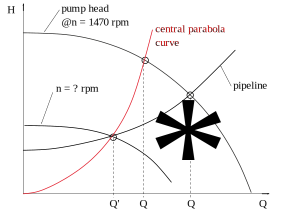
\includegraphics{Problem_solving/figs/PS_OperatingPoint_Affinity.png}}\\
	\end{center}
    \end{minipage}
& 

\begin{minipage}{6cm}

\noindent Solution: 

\begin{itemize}
\item The ac\-tual wor\-king point is given by the so\-lu\-tion of $H_{pump}=H_{pipe}$, which gives $Q=0.08 [m^3/s]$ and $H=27.2[m]$.
\item Affinity states that while varying the revolutionary speed, $H/n^2$ and $Q/n$ remain constant. Thus, also $H/Q^2$ remains constant, let's denote this constant by $a$. So, while varying the revolutionary speed, the working point moves along the \emph{central parabola} (see figure), given by $H_{ap}=a\,Q^2$.
\end{itemize}
\end{minipage}
\end{tabular}

However, as $Q'$ is given and we also know that this point has to be located on the pipeline characteristic, we know that $H'= 20+1125 \cdot 0.05^2=22.81[m]$. Thus, the parameter of the affine parabola is $a=H'/Q'^2=9125$. 

$Q^*$ is given by the intersection of the affine parabola and the original pump characteristic: $H_{ap}(Q^*)=H_{pump}(Q^*)$, which gives $Q^*=0.06148[m^3/s]$ with $H^*=34.5[m]$.

Now we can employ affinity between $Q^*$ and $Q'$:

\begin{equation*}
n'=n^*\frac{Q'}{Q^*}=1470\times \frac{0.05}{0.06148}=1195.5 [rpm] 
\end{equation*}

and just for checking the calculation

\begin{equation*}
H'=H^* \left(\frac{n'}{n^*} \right)^2=34.5\times \frac{1195.5^2}{1470^2}=22.81 [m].
\end{equation*}

%%%%%%%%%%%%%%%%%%%%%%%%%%%%%%%%%%%%%%%%%%%%%%%%%%%%%%%%%%%%%%%%%%%%

\vspace{1cm}
\noindent {\bf Problem \thesection.\theprob}\stepcounter{prob}

Solve the previous control problem (pump: $H_{pump}=45-2781 Q^2$, pipeline: $H_{pipe}=20+1125Q^2$, desired flow rate: $Q'=0.05 [m^3/s]$) using a throttle at the pressure side of the pump and also with a bypass line. Compare the resulting operations in terms of power loss!

\begin{figure}[!ht]
\centering
\includegraphics[width=0.7\textwidth]{Problem_solving/figs/PS_Control1.png}
\end{figure}

%%%%%%%%%%%%%%%%%%%%%%%%%%%%%%%%%%%%%%%%%%%%%%%%%%%%%%%%%%%%%%%%%%%%%%

\vspace{1cm}
\noindent {\bf Problem \thesection.\theprob}\stepcounter{prob}

A pump, whose characteristic curve is given by $H_{pump}=70-90000[s^2/m^5]Q^2$, works together with two parallel pipes. The main pipe is given by $H_1=30+100000[s^2/m^5]Q^2$. Calculate the head-flow relationship $H_2(Q)$ of the side pipe, whose opening results in a flow rate of $480[l/min]$ in the main pipe. The static head of the second side pipe is $25[m]$.

\noindent Solution: 

\begin{itemize}
\item Head of the main pipe at the prescribed flow rate: $Q_1 = 480[l/min]=0.008[m^3/s] \quad \rightarrow \quad H_1(Q_1)=36.4[m]$
%
\item The head is the same, so the flow rate of the pump is
 $H_p(Q_p)= H_1(Q_1) \quad \rightarrow \quad Q_p=\sqrt{\frac{70-36.4}{90000}}=0.0193[m^3/s]$
%
\item Thus, the flow rate on the side pipe is $Q_2=Q_p-Q_1=0.0193-0.008=0.0113[m^3/s]$
%
\item The actual characteristic of the side pipe: $H_2(Q_2)=25+aQ_2^2=36.4[m] \quad \rightarrow \quad a=\frac{36.4-25}{0.0113^2}=89279$
%
\item The solution is $H_2(Q_2)=25+89279 Q^2$.
\end{itemize}

%%%%%%%%%%%%%%%%%%%%%%%%%%%%%%%%%%%%%%%%%%%%%%%%%%%%

\vspace{1cm}
\noindent {\bf Problem \thesection.\theprob}\stepcounter{prob}

Pumps $I$ and $II$ feed pipes $1$ and $2$ shown in the figure below. Their characteristics are:
\begin{eqnarray}
	&& H_I = 45m-24900s^2/m^5Q^2 \nonumber \\
	&& H_{II} = 35m-32200s^2/m^5Q^2 \nonumber \\
	&& H_1 = 10m+4730s^2/m^5Q^2 \nonumber \\
	&& H_2 = 15m+8000s^2/m^5Q^2\nonumber
\end{eqnarray}
Find the flow rates and heads if valve $"V"$ is closed, and if it it opened. 
0.023054084926172
% (Solution: closed: $H=34.46~\mathrm{m},~Q=0.02578~\frac{\mathrm{m^3}}{\mathrm{s}}$; open:  $H=25.18\mathrm{m},~Q=0.03567~\frac{\mathrm{m^3}}{\mathrm{s}}$)
(Solution: closed: $H=31.766~\mathrm{m},~Q=0.02305~\frac{\mathrm{m^3}}{\mathrm{s}}$; open:  $H=25.18\mathrm{m},~Q=0.03567~\frac{\mathrm{m^3}}{\mathrm{s}}$)

\begin{figure}[!ht]
\centering
\includegraphics{Problem_solving/figs/PS_Control_Pumps.png}
\end{figure}

%%%%%%%%%%%%%%%%%%%%%%%%%%%%%%%%%%%%%%%%%%%%%%%%%%%%%%%%%%%%%%%%%%%%%%%%%%
\vspace{1cm}
\noindent {\bf Problem \thesection.\theprob}\stepcounter{prob}

Two pumps, $H_1=70m-50000s^2/m^5Q^2$ and $H_2=80m-50000s^2/m^5Q^2$ can be coupled parallel or in series. Which arrangement will deliver more liquid through the pipe $H_p=20m+25000s^2/m^5Q^2$? (Solution: in series: $Q=0.03224~\frac{\mathrm{m^3}}{\mathrm{s}},~H=46~\mathrm{m}$; in parallel: $Q=0.03818~\frac{\mathrm{m^3}}{\mathrm{s}},~H=56.44~\mathrm{m}$)

%%%%%%%%%%%%%%%%%%%%%%%%%%%%%%%%%%%%%%%%%%%%%%%%%%%%

\vspace{1cm}
\noindent {\bf Problem \thesection.\theprob}\stepcounter{prob}

Pump S, with the characteristitc curve $H_S=37-0.159Q^2$, is feeding an irrigation system consisting of parallel pipes. The units are $Q[m3/h]$ and $H[m]$. Each pipe contains at its end a sprinkler. The pipes are $20m$ long, their inner diameter is $25mm$, the friction coefficient is $0.03$. The sprinklers discharge $4 m^3/h$ water at $2 bar$ overpressure, their characteristics can be written as $H_{spr}=K_{spr}Q^2$. 

\begin{itemize}
\item Draw the sketch of the irrigation system with 3 parallel pipes!
\item How much water is discharged if only one pipe is in operation?
\item How many parallel pipes can be fed if the overpressure before the sprinklers must be $2 bar$? 
\end{itemize}

(Solution: single pipe: $Q_1 = 4.5~\frac{\mathrm{m^3}}{\mathrm{h}}$, $H=33.7~\mathrm{m}$; the pump can supply 2 pipes only)

%%%%%%%%%%%%%%%%%%%%%%%%%%%%%%%%%%%%%%%%%%%%%%%%%%%%

\vspace{1cm}
\noindent {\bf Problem \thesection.\theprob}\stepcounter{prob}

The characteristics of a pump supplying a small village with water is $H_p=70-330Q^2$. The village network is modeled by the curve $H_{cd}=25+30Q^2$ during the day while the night operation can be described by $H_{cn}=25+750Q^2$. A high water tower is attached to the delivery tube of the pump, its characteristics is $H_T=40-55|Q|Q $. Here $Q$ is positive if water flows down from the tower. The units in the formulae are [Q] = m3/s; [H] = m. Draw a sketch of the water system. Find the flow rates of the pump, village and tower both for day and night operation. Find the head of the pump both for day and night! Use a millimeter paper to draw the charasteristics curves! (Solutions: $Q_{pump}=0.33m^3/s$ and $0.29m^3/s$; $Q_{village}=0.6m^3/s$ and $0.15m^3/s$; $Q_{tower}=0.275m^3/s$ and $-0.14m^3/s$. $H_{pump}=36m$ and $41m$.)
%%%%%%%%%%%%%%%%%%%%%%%%%%%%%%%%%%%%%%%%%%%%%%%%%%%%

\vspace{1cm}
\noindent {\bf Problem \thesection.\theprob}\stepcounter{prob}

How much water is delivered by the pump $H_p=70-45000Q^2$ through the pipe system $H_s = 20+20000Q^2$ ? The flow rate must be reduced to $0.015 m^3/s$. This can be done either by throttling control or by using a by-pass control. Draw the pump-pipe-valve arrangements for both cases. How large is the hydraulic loss in the valves in the first and in the second case? The power consumption of the pump is $P_{input} = 9.4+240Q-50000Q^2$. How large is the specific energy consumption $f$ in the two cases? The units in the formulae are: $[m], [m^3/s], [kW]$. (Solution: $Q= 0.0277~\frac{\mathrm{m^3}}{\mathrm{s}}$, $P_{throttle}' = 5.2~\mathrm{kW}$, $P_{bypass}'=4.0~\mathrm{kW}$, $\mathrm{SEC}=0.237~\frac{\mathrm{kWh}}{\mathrm{m^3}}$ and $\mathrm{SEC}=0.285~\frac{\mathrm{kWh}}{\mathrm{m^3}}$, respectively.)




% SERIAL AND PARALLEL CONNECTIONS %%%%%%%%%%%%%%%%%%%%%%%%%%%%%%%%%%%%%%%%%%%%%
\section{Pumps and pipes connected in series or parallel}

In Sec.\,\ref{sec:head_discharge_curves_and_operating_point}, the determination of the operation point of a single pump working to a single hydraulic system is discussed in details, see also Fig.\,\ref{fig:SimplePumpingSystem}. In many cases, however, the flow rate $Q_s$ or the head $H_s$ required by the system cannot be satisfied by a single pump efficiently. Or it is much more feasible economically (e.g., investment costs) to use several smaller pumps instead of a single much larger one. The pumps can be connected in a serial or in a parallel way. Each has its own specific application/purpose: increase the flow rate (parallel) or increase the produced head (serial) when the required pressure difference of the system is high (e.g., large height differences). The difficulty in both cases is the determination of the equivalent characteristic curve of the coupled pumps to be able to find the operation point with the system. This is the main topic of the forthcoming sections. Figure\,\ref{fig:pump_stations_examples} shows two pump stations with pumps connected in a parallel (left-hand side) and in a serial (right-hand side) way. In more complex pump stations, the mixture of serial and parallel connections of pumps can also be found depending on the technological needs.

\begin{figure}[ht!]
	\centering
		\includegraphics[height=4.5cm]{Control/Figures/Pump_Station_Parallel_Connection.jpg}
		\includegraphics[height=4.5cm]{Control/Figures/Pump_Station_Serial_Connection.jpg}
	\caption{Pump stations with pumps connected in parallel (left) and in series (right).}
	\label{fig:pump_stations_examples}
\end{figure}

From the system point of view, it is also possible that a pump (or a pump station) have to provide flow rates (and head) to different systems or a single but a complex system. In general, a system might also be composed by several subsystems built-up by a mixture of serial and parallel connections (similarly to pump stations), where each subsystem has its own characteristic curves. Again the difficulty is the derivation of an equivalent characteristic curve of the whole systems.

From sizing point of view, the system of a technology or an industrial project is usually/mainly given, and the specific needs of the application drive its design. On the other hand, a pump station has to be designed according to the needs of the given hydraulic systems. Naturally, it might also be possible that modifications on the system have to be carried out for efficiency reasons, and the complete design is an iterative process.

%------------------------------------------------
\subsection{Theory of serial connection}
In order to intorduce the basics of serial connections, consider two pump connected in series, and working to a single system. The block diagram of such a configuration is presented in Fig.\,\ref{fig:block_diagram_serial_connection}. Due to the principle of conservation of mass, the volue flow rate (assuming inclompressible flow) of the three hydraulic elements (the two pumps and the system) must be equal, and denoted simply by $Q$. In contrast, the head ``production'' of the pumps are additive; that is, the overall head of the two pumis is
%
\begin{equation}
H_{p3} = H_{p1} + H_{p2}.
\end{equation}
%
Keep in mind that the head can always be reagarded as presusre difference since $H_p \approx \rho g \Delta p_p$, where $\rho$ is the density and $g$ gravitational acceleration. In this sense, the pressure elevated by the first pump is further increased by the second pump. The overall pressure difference produced by the pumps (sum of the heads) is completely consumed by the system. This is the basis of operating point introduced in Sec.\,\ref{sec:head_discharge_curves_and_operating_point}. Mathematically, the solution of the algebraic equation
%
\begin{equation} \label{principle_of_serial_connection}
H_{p3}(Q) = H_{p1}(Q) + H_{p2}(Q) = H_s(Q)
\end{equation}
%
yields the flow rate $Q^o$ and head $H^o$ of the operating point.

\begin{figure}[ht!]
	\centering
		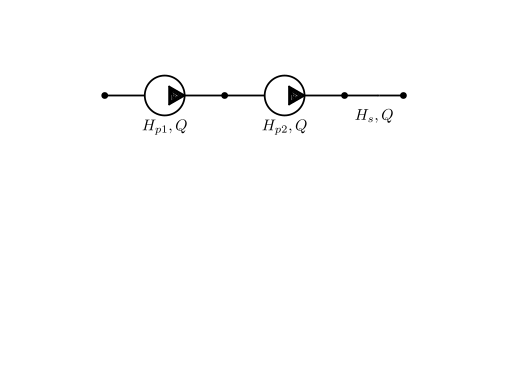
\includegraphics[height=1.25cm]{Control/Figures/Block_Diagram_Serial_Connection.pdf}
	\caption{Block diagram of two pumps connected in series, and working to a single system.}
	\label{fig:block_diagram_serial_connection}
\end{figure}

To be specific, the characteritic curves of the pumps and the system is summatized as follows
%
\begin{align}
H_{p1}(Q) &= A_{p1} - B_{p1} Q^2 = 80 -  80000 Q^2, \label{pump1_characteristic_curve_serial} \\
H_{p2}(Q) &= A_{p2} - B_{p2} Q^2 = 40 -  60000 Q^2, \label{pump2_characteristic_curve_serial} \\
H_s(Q)    &= A_s    + B_s    Q^2 = 60 + 400000 Q^2, \label{system_characteristic_curve_serial}
\end{align}
%
where the units of the head $H$ and the volume flow rate $Q$ are $\mathrm{m}$ and $\mathrm{m^3/s}$, respectively. The general form of such charateristic curves via the constants $A_i$ and $B_i$ are discussed already in Sec.\,\ref{sec:real_performance_curves_turbomachines} and Sec\,\ref{sec:head_discharge_curves_and_operating_point}; thus, it is not repeated here. The left-hand side of Fig.\,\ref{fig:example_serial_connection} represents the functions defined by Eqs.\,\eqref{pump1_characteristic_curve_serial}-\eqref{system_characteristic_curve_serial} by the black (pumps) and the red (system) curves.

\begin{figure}[ht!]
	\centering
		\includegraphics[width=8cm]{Control/Figures/TheorySerialConnection.png}
		\includegraphics[width=8cm]{Control/Figures/TheorySerialConnection_SamePumps.png}
	\caption{A typical characteristic curve of a spring-loaded pressure relief valve. Left: the volume flow rate $Q_{prv}$ as a function of the pressure difference $\Delta p$. The theoretical (black) curves are also depicted. Right: the pressure difference $\Delta p$ as a function of the flow rate $Q_{prv}$.}
	\label{fig:example_serial_connection}
\end{figure}

Tha main task is to unite the two characteristic curves of the pumps in order to determine the operation point. According to Eq.\,\eqref{principle_of_serial_connection}, it is simply the summary of the heads. As the characteristic curves are already expressed for the heads in Eqs.\,\eqref{pump1_characteristic_curve_serial}-\eqref{system_characteristic_curve_serial}, the overall characteristic curve of the two pumps can be obtained analitically very easily:
%
\begin{equation}
\begin{split}
H_{p3}(Q) &= H_{p1}(Q) + H_{p2}(Q), \\
          &= 80 - 80000 Q^2 + 40 - 60000 Q^2, \\
		  &= 120 - 140000 Q^2,
\end{split}
\end{equation}
%
shown by the blue curve in Fig.\,\ref{fig:example_serial_connection}. The operating point of the whole hydraulic sstem is at the intersection of the blue and the red curves marked by the big black cross. Numerically, the volume flow rate of the operation point $Q^o$ can be calculated by equating the two characteristic curves:
%
\begin{equation}
\begin{split}
         H_{p3}(Q^o) &= H_{s}(Q^o), \\
120 - 140000 (Q^o)^2 &= 60 + 400000 (Q^o)^2, \\
		          60 &= 540000 (Q^o)^2, \\
			     Q^o &= \sqrt{\frac{60}{540000}} = 0.01054\,\mathrm{\frac{m^3}{s}}.
\end{split}
\end{equation}
%
The head of the system cab be claculated by substituting the flow rate of the operating point $Q^o$ into Eq.\,\eqref{system_characteristic_curve_serial}:
%
\begin{equation} \label{principle_of_serial_connection}
H_s^o = A_s + B_s Q^2 = 60 + 400000 (Q^o)^2 = 104.4\,\mathrm{m}.
\end{equation}
%
since the same volume flow rate $Q^o$ flows through both pumps, their individual operation point is at the crossing of the red vertical line at $Q^o$ with the charcteristic curves, see the small black crosses in the left-hand side of Fig.\,\ref{fig:example_serial_connection}. Again, the heads of the operating points of the pumps can be obtaines by subtitution:
%
\begin{align}
H_{p1}^o &= A_{p1} - B_{p1} Q^2 = 80 - 80000 (Q^o)^2 = 77.1\,\mathrm{m}, \\
H_{p2}^o &= A_{p2} - B_{p2} Q^2 = 40 - 60000 (Q^o)^2 = 33.3\,\mathrm{m}.
\end{align}
%
With the above-described calculations, all the properties (heads and flow rates) of all the elements of the whole hydraulic system could be obtained, see also the lables in the left-hand side of Fig.\,\ref{fig:example_serial_connection} pointig to the projetions to the horizontal and vertical by the red thin lines.

In some cases, it may happen that the characteristic curves are not given in an analitical form; for instance, only a graphical curve is given in an old catalouge or only some measured points are available. In this case, there is an alternative, graphical solution to approximate the operating point. The first step is the division of the volume flow rate range into a discrete set of values represented by the vertical dashed lines in Fig.\,\ref{fig:example_serial_connection} left. Second, evaluate the pump and the system charaterictic curves at these flow rate values (see the black and red dots). It is possible that this process is already done by a measurement. Next, the equivalent charateristic curve of the two pumps can be obtained by summing the values of the heads of the black dots at a given dashed line, and mark the corresponding point on the same dashed line. The result is the series of blue dots in Fig.\,\ref{fig:example_serial_connection} left. Drawing (by hand) the approximated charateristic curves through the calculated dots, the intersection of the blue and the red curves will define the estimated operating point as usual. Finally, the projection via the thin red lines, the values of the operating heads and flow rates of the individual pumps and the system can be determined as well.







%------------------------------------------------
\subsection{Theory of parallel connection}

%------------------------------------------------
\subsection{Operation point of complex connections}

%------------------------------------------------
\subsection{Problems}

%%%%%%%%%%%%%%%%%%%%%%%%%%%%%%%%%%%%%%%%%%%%%%%%%%%%

\noindent {\bf Problem \thesection.\theprob}\stepcounter{prob}

The performance curve of a pump is $H_p = 70-10000\,Q^2$. This pump is connected to two pipe systems with characteristic curves $H_{s1} = 5000\,Q^2+10$ and $7500\,Q^2+15$. In these formulae, the head is in meters, and the unit of the volumetric flow rate is $\frac{\mathrm{m^3}}{\mathrm{s}}$. Find the operation point, if the two pipe systems are connected (a) in series, or (b) in parallel to the pump. Draw the performance curves in both cases!

Solution: when the pipe systems are in series connection, the volumetric flow rate through them is the same, and in the calculation of the performance curves, the heads are summed at each volumetric flow rate. This means:
\begin{equation*}
H_{s,ser} = H_{s1} + H_{s2} = 12500\,Q^2+25.
\end{equation*}
In the operation point, the head of the pump equals the head required by the system:

\begin{align*}
& H_{s,ser} = H_p, \\
& 12500\,Q^2+25=70-10000\,Q^2,\\
& Q_{ps} = \sqrt{\frac{45}{22500}} = 0.04472~\frac{\mathrm{m^3}}{\mathrm{s}}, \\
& H = H_p(Q_{ps}) = H_{s,ser} = 70 - 10000\cdot 0.04472^2 = 50~\mathrm{m}.
\end{align*}

When the two pipe systems are connected in parallel, the pressure drop/head is the same on them, while their volumetric flow rates are different. In this case, to calculate the characteristic curve of the total system, the volumetric flow rates should be summed at each head. To do this,  we need to rearrange the performance curves to be functions of the head:
\begin{align*}
& H_p = 70-10000\,Q^2 \rightarrow Q_p = \frac{\sqrt{70-H}}{100} \\
& H_{s1} = 5000\,Q^2+10 \rightarrow Q_{s1} = \frac{\sqrt{2}\,\sqrt{H-10}}{100} \\
& H_{s2} = 7500\,Q^2+15 \rightarrow Q_{s2} = \frac{\sqrt{3}\,\sqrt{H-15}}{150} .
\end{align*}
Note that the expressions above are only valid for a certain $H$ interval, since the argument of the square root function cannot be negative. Calculating the sum of the two parallel pipes, then equating the pump and the system, solving for $H$, the operating point can be identified:
\begin{align*}
& Q_{s,par} = Q_{s1} + Q_{s2} = \frac{\sqrt{2}\,\sqrt{H-10}}{100}+\frac{\sqrt{3}\,\sqrt{H-15}}{150}  = Q_p = \frac{\sqrt{70-H}}{100}\\
& H =  20.03~\mathrm{m}, \\
& Q = 0.07069~\frac{\mathrm{m^3}}{\mathrm{s}}.
\end{align*}

The performance curves are displayed in Figure \ref{fig_example1}.

\begin{figure}[!htb]
\centering
\includegraphics[width=0.8\textwidth]{figs/problem_5_par_1.png} 
\caption{ Performance curves of the problem. The circles denote the operation points.}
\label{fig_example1}
\end{figure}

%%%%%%%%%%%%%%%%%%%%%%%%%%%%%%%%%%%%%%%%%%%%%%%%%%%%

\vspace{1cm}
\noindent {\bf Problem \thesection.\theprob}\stepcounter{prob}

Two pumps, with performance curves $H_{p1} = 50 - 30000\cdot Q^2$ and $H_{p2} =  40 - 20000\cdot Q^2$ are conveying water through a pipe system that's characteristic curve is $H_s = 3 + 7250\cdot Q^2$. Find the operating points if the two pump are connected (a) in series or (b) in parallel! (Solution: $H_{ser} = 14.02~\mathrm{m}$, $Q_{ser} = 0.03898~\frac{\mathrm{m^3}}{\mathrm{s}}$, $H_{par} = 25.43~\mathrm{m}$, $Q_{par} = 0.05562~\frac{\mathrm{m^3}}{\mathrm{s}}$)

%%%%%%%%%%%%%%%%%%%%%%%%%%%%%%%%%%%%%%%%%%%%%%%%%%%%
%peldatar 6.1

\vspace{1cm}
\noindent {\bf Problem \thesection.\theprob}\stepcounter{prob}

A pump that's performance curve is $H_I (\mathrm{m}) = 70 - 50000 \frac{\mathrm{s^2}}{\mathrm{m^5}} Q^2$, conveys water through a pipe system with characteristic curve $H_s (\mathrm{m}) = 20 + 10000 \frac{\mathrm{s^2}}{\mathrm{m^5}} Q^2$. Find the volumetric flow rate! The volumetric flow rate is increased to $Q=0.032~\frac{\mathrm{m^3}}{\mathrm{s}}$, using a second pump with performance curve $H_{II} (\mathrm{m}) = 80 - 50000 \frac{\mathrm{s^2}}{\mathrm{m^5}} Q^3$. The operating point of the system is set by a throttle valve at the pressure side. How would the loss power be smaller: if the two pumps were connected in series or in parallel? (Solution: $Q=0.0285~\frac{\mathrm{m^3}}{\mathrm{s}}$, $P_{ser}' = 5.45~\mathrm{kW}$, $P_{par}' = 9.88~\mathrm{kW}$)

%%%%%%%%%%%%%%%%%%%%%%%%%%%%%%%%%%%%%%%%%%%%%%%%%%%%

\vspace{1cm}
\noindent {\bf Problem \thesection.\theprob}\stepcounter{prob}

Two pump operate in parallel. The performance curve of the first pump and it's pressure side pipeline is the following: $H_{pI} = 40 - 0.17Q^2$, $H_{s,I} = 5 + 0.4Q ^2$; the data for the second pipe is $H_{pII} = 27 - 0.135Q^2$, $H_{s,II} = 0.8Q ^2$. The head in in meters, and the unit of the volumetric flow rate is $\frac{\mathrm{m^3}}{h}$. These two pipes are joined, and convey water through a third pipeline with characteristic curve $H_{s,III} = -3 + 0.63Q ^2$. Find the operating point! (Solution: $Q = 6.473~\frac{\mathrm{m^3}}{h}$, $H=23.4~\mathrm{m}$.)

% WATER HAMMER, HYDRAULIC TRANSIENTS %%%%%%%%%%%%%%%%%%%%%%%%%%%%%%%%%%%%%%%%%%
\section{Water hammer, hydraulic transients}

Up to this point, turbomachinery is discussed from a stationary operation point of view. Such a discussion have its own right, since most of its lifetime, an installation operates in steady-state fashion. One of the main reasons is the efficiency: a device is usually designed to operate efficiently over a specific parameter range around the designed operation point. Thus, a significant deviation from this optimal point can considerably increase the operating costs or needs expensive additional equipment to overcome this issue. The previous sections of this chapter are devoted to this problem. Moreover, transient operations are usually causing greater wear of the elements of a device, which might result in a lower lifetime and additional maintenance and investment costs.

We shall see in this section that transient phenomenon in a hydraulic system also plays a significant role, although its timespan is usually many orders of magnitude smaller than steady-state operations. The starting and stopping of hydraulic machinery are two natural examples. The phenomenon discussed in this section is the generated pressure surge or wave by the sudden closure of a valve. This pressure wave, having even tenths of bars peak value, can cause major problems; for instance, the rupture or the collapse of a pipe. Transients can also be generated in a domestic environment by the sudden close (e.g., within a fraction of a second if it is allowed by design) of the faucet in the bathroom or the kitchen. The vibration of the pipeline system for a few seconds and even a small blow at the tap might be observable. Such an effect needs to be avoided at all costs in industrial environments. Since the peak amplitude of the pressure is usually much higher due to the much larger mass of liquid involved during the process.

%------------------------------------------------
\subsection{Introduction to the transient phenomenon in pipes} \label{sec:introduction_to_transient_phenomenon}
Consider a pipeline in steady-state operation, i.e. with constant flow rate (constant flow velocity). In order to regulate the flow rate, a valve is placed at the end of this pipe, see the left-hand side of Fig.\,\ref{fig:water_hammer}. Let us assume a limit case where the valve is suddenly (infinitely fast) closed. Naturally, the huge mass of moving liquid in the pipe cannot stop immediately; it still moves towards the end of the pipe. However, the fluid packages at the valve are already stopped. The result is an initiated compression (pressure) wave propagating along the pipe with sonic velocity (sound speed) $a$, see the diagrams in Fig.\,\ref{fig:water_hammer} below the schematic drawings of the pipe-reservoir systems. The pressure wave is often referred to as \emph{shock wave} or positive surge, and its magnitude (amplitude) is denoted by $\Delta p$. This pressure amplitude $\Delta p$ (flux of momentum) built up in the system covers the energy required to stop the liquid particles. That is, before the shock front, the liquid is still moving, while after the shock front, the liquid is already stopped. By analogy, the propagation of the pressure wave with a finite speed of $a$ is a similar phenomenon as the propagation of a voice in the air via pressure waves (compression or depression of air). Any information in a system can be transferred only with a finite speed. Another kind of analogy is when the first wagon of a moving train hits the bumper and stops. The rest of the wagons, connected by springs, are still moving, and they stop one by one, one after another. Here, the information (stop of the train) is again propagating with a finite speed along the wagons. Also, the generated ``pressure wave'' is a compression wave in a sense that the springs connecting the wagons are compressed.

Now consider a similar pipeline system, but the valve served to regulate the flow rate is placed at the beginning of the pipe rather than at its end. The situation is similar to the case described above. The main domain of liquid is still moving, while the fluid particles at the valve are already stopped (at the moment of the closure). The difference is that a \emph{depression wave} $\Delta p$ (the absolute value of the pressure is below the system pressure) is build up that tries to disrupt the fluid particles. The speed of the shock front propagation $a$ is approximately the same as in case of the compression wave discussed above. According to the train analogy, the last wagon of a moving train is stopped, while the rest of the wagons are again stopped only one by one, one after another. However, here the springs connecting the wagons are stretched. That is, the initiated wave is a depression wave.

\begin{figure}[h!]
\centering
%\begin{wrapfigure}{r}{0.6\textwidth}
\includegraphics[width=0.8\textwidth]{figs/water_hammer_CV.pdf}
\caption{\label{fig:water_hammer}Water hammer; sudden closure at the (left) end of the pipe and (right) beginning of the pipe.}
%\end{wrapfigure}
\end{figure}

In real situations, the infinitely fast closure of a vale cannot be realised. Instead, a valve is closed by a certain amount of finite time, causing a certain amount of velocity difference ($\Delta v$) in the fluid flow. That is, the liquid is not perfectly stopped; only its velocity is changed. In order to achieve the generated velocity difference, a pressure wave (compression or depression) that provides the energy necessary to decrease the liquid velocity must be built up in the system. The speed of the propagation of the shock front is still $a$. That is, even though the valve is not totally closed, pressure waves with large amplitude can still be presented in the system.

In order to ``feel'' how much energy is contained in a fluid flow in a pipeline, consider a typical configuration of an $L=1\,\mathrm{km}$ long pipe with a diameter of $D=200\,\mathrm{mm}$. Assume that the liquid is water with density $\rho=1000\,\mathrm{kg/m^3}$. The mass of the liquid in the pipe is
%
\begin{equation}
m = \rho L \frac{D^2 \pi}{4} \approx 31.4\,\mathrm{t}.
\end{equation}
%
In order to change the velocity of this mass of water by $\Delta v=1\,\mathrm{m/s}$ within $t=1\,\mathrm{s}$, the required amount of power is
%
\begin{equation}
P = \frac{E_{kin}}{t} = \frac{1}{t} \frac{1}{2} m \Delta v^2 \approx 15.7\,\mathrm{kW},
\end{equation}
%
where $E_{kin}$ is the kinetic energy difference of the liquid.

With the above-described introduction, a quick overview of the phenomenon could be provided. In the rest of the section, we shall proceed with specific calculations and try to answer the following questions. How can the speed of sound $a$ in a pipe or of a pure liquid be calculated? What is the magnitude $\Delta p$ of the generated pressure wave? Furthermore, how it is related to the speed of sound $a$ and the velocity difference $\Delta v$? Finally, how can we avoid/soften the generation of such a pressure wave?

%------------------------------------------------
\subsection{The sound speed in liquids and in pipes}
The propagation of sound (or signal) in any medium is inherently related to the compressibility. In case of an absolutely rigid material (naturally, this assumption is always hypothetical), the sound speed is infinite. That is, any disturbance at a point appears immediately at another point of the material. This is the case for incompressible liquids. Although in many cases, the assumption of incompressibility is a reasonable simplification, in reality, every material is compressible; therefore, a finite speed of sound exists. From thermodynamics, it is well-known that the speed of sound can be calculated from the constitutive law (equation of state) of a substance. For water, the simplest equation of state can be written as
%
\begin{equation} \label{WaterEquationOfState}
p = p_0 + E_f \frac{\rho - \rho_0}{\rho_0},
\end{equation}
%
where $p$ is the pressure, $E_f$ is the bulk (elasticity) modulus of the fluid, and $\rho$ is the density. The subscript $0$ indicates a reference point where both the pressure $p_0$ and the density $\rho_0$ are known. Equation\,\eqref{WaterEquationOfState} expresses a linear relationship between the pressure $p$ and density $\rho$. Observe that the density is increasing with increasing pressure. The second power of the speed of sound can be obtained from the following partial derivative:
%
\begin{equation}
a^2 = \frac{\partial p}{\partial \rho} \approx \frac{\Delta p}{\Delta \rho}
\end{equation}
%
expressing how much pressure difference is necessary to change the density by a single unit. Performing the partial derivative on Eq.\,\ref{WaterEquationOfState}, the speed of sound reads as
%
\begin{equation}
a = \sqrt{ \frac{E_f}{\rho_0} } \approx \sqrt{ \frac{E_f}{\rho} }.
\end{equation}
%
If the density does not change much during the compression/depression, $\rho_0$ can be replaced by a simple mean value of the density denoted by $\rho$. For water, the value of the bulk modulus is approximately $E_f=2.1\,\mathrm{GPa}$, the density is approximately $\rho=1000\,\mathrm{kg/m^3}$; thus, the speed of sound for pure water is about $a=1449\,\mathrm{m/s}$.
 
The above-derived value for sound propagation is valid only for rigid pipes when the elasticity modulus of the pipe is much higher than that of water. If this is not the case, the speed of sound is significantly altered. Due to the elevated (decreased) pressure, the diameter of the pipe is increased (decreased) via elastic deformation. The change in the volume of the pipe acts as if the fluid became more compressible. Note that due to the change of the cross-section, more fluid can be pushed into the pipe. In order to take into account the elasticity of the pipe, a reduced elastic modulus $E_r$ is written as
%
\begin{equation}
\frac{1}{E_r} = \frac{1}{E_f} + \frac{D}{\delta E_p},
\end{equation}
%
where $D$, $\delta$ and $E_p$ are the diameter, thickness and the elastic modulus of the pipe, respectively. Typical values for $E_p$ are ranging between $600\,\mathrm{MPs}$ and $900\,\mathrm{MPa}$. The reduced speed of sound is now defined as
%
\begin{equation}
a = \sqrt{ \frac{E_r}{\rho} }.
\end{equation}
%
Consider a pipe with a diamater of $D=110\,\mathrm{mm}$ and a thickness of $\delta=18.3\,\mathrm{mm}$ with $E_p=800\,\mathrm{MPa}$, the speed of sound is reduced to $a=354\,\mathrm{m/s}$.

%------------------------------------------------
\subsection{Allievi principle: the pressure amplitde for fast closure} \label{sec:pressure_amplitude_fast_closure}

In order to develop sizing equations to avoid water hammer problems, the relationship between the amplitude of the generated pressure wave $\Delta p$ and the velocity change $\Delta v$ need to be found. For this, the macroscopic balances of mass and momentum around the shock front are formulated; and with reasonable simplifications, the required expression shall be established. Consider a frame of reference (co-ordinate system) moving along the pipe together with the shock front with speed $a$. For a better visibility, the related picture in the bottom of Fig.\,\ref{fig:water_hammer} is magnified in Fig.\,\ref{fig:allievi_principle}; thus, additional notations can be added without overcrowding the figure. The vertical dashed line denotes the shock front itself. On the left-hand side of the shock, the pressure and density are $p$ and $\rho$, respectively. The cross-section of the pipe is $A_1$, where the vector $dA_1$ denote the surface element vector. The velocity at this pipe section is $v+a$. The addition of $a$ is necessary as our co-ordinate system is moving with a speed of $a$. Therefore, the two velocities must be added together. On the right-hand side of the shock, the pressure and the density are elevated by $\Delta p$ and $\Delta \rho$, respectively. Moreover, the velocity of the fluid flow is reduced by $\Delta v$. The resulted outflow velocity from the investigated pipe section is $v-\Delta v + a$. Observe that due to the moving reference frame, the addition $a$ is again necessary. The cross-section in the right-hand side is $A_2$ and the corresponding surface element vector is $dA_2$. Due to the increased pressure after the shock front (righ-hand side), the cross section $A_2$ is larger than that of in the left-hand side $A_1$. The difference is $\Delta A = A_2 - A_1$ located at the shock front as a ring shaped surface. Its surface element vector is marked by $d\Delta A$.

\begin{figure}[h!]
\centering
%\begin{wrapfigure}{r}{0.6\textwidth}
\includegraphics[width=0.6\textwidth]{figs/WaterHammer_AllieviPrinciple.pdf}
\caption{\label{fig:allievi_principle}Shock front in a moving frame reference with speed $a$. The pressure wave is generated by a sudden closure of a valve at the end of the pipe.}
%\end{wrapfigure}
\end{figure}

From elementary fluid dynamics, it is well-know that the macroscopic momentum balance for the fluid package bounded by the red dashed line in Fig.\,\ref{fig:allievi_principle} in an integral form reads as
%
\begin{equation} \label{macroscopic_momentum_balance}
\frac{\partial}{\partial t} \int_V \left(\rho \underline{v} \right) dV + \int_A \rho \underline{v} \left( \underline{v} \cdot d\underline{A} \right) + \int_A p d\underline{A} = \int_V \rho \underline{g} dV.
\end{equation}
%
This integral equation express that the momentum of the bounded fluid package can be changed by forces acting on the bounding surfaces (e.g., pressure, inertia) and on the volume (e.g., gravity). In this equation, $\underline{v}$ denote the velocity vector at a given point on the surface or in the volume in general. In the moving frame co-ordinate system, the fluid flow is stationary; thus, the first integral is identically zero. Moreover, let us neglect the effect of gravity; consequently, the last integral in the right-hand side of Eq.\,\eqref{macroscopic_momentum_balance} is zero as well. The simplified equation is
%
\begin{equation} \label{macroscopic_momentum_balance_simplified}
\int_A \rho \underline{v} \left( \underline{v} \cdot d\underline{A} \right) + \int_A p d\underline{A} = 0.
\end{equation}
%
Observe that in the surface integrals, the surface elements $d\underline{A}$ are vectors, and they are pointing in the outward direction (by convention). In general, performing the integrations in Eq.\,\eqref{macroscopic_momentum_balance_simplified} is a cumbersome task. However, assuming that the velocity vectors are constants (using the mean velocity at every point of the cross-sections) and that they are always perpendicular to the cross-sections, the integrations can be done by elementary calculations. That is, they become simple multiplications of the magnitude of the integrands and the area of the surfaces. It must be stressed that the proper sign of the vectors has to be taken into account. Demonstrate this with an example:
%
\begin{equation}
\int_{A_1} \rho \underline{v} \left( \underline{v} \cdot d\underline{A}_1 \right) = - \rho \left( v+a \right)^2 A_1.
\end{equation}
%
The magnitude of general velocity vector $\underline{v}$ is $v+a$ at cross-section $A_1$. Let the positive direction denoted by $x$, see Fig.\,\ref{fig:allievi_principle}. As the surface element vector $d\underline{A}_1$ is pointing to the negative direction, the value of the integral is negative. Keep in mind that the second power of the velocity vector is always positive regardless of its actual direction. Performing all the integrations in Eq.\,\ref{macroscopic_momentum_balance_simplified} in a similar way for the surfaces $A_1$, $A_2$ and $\Delta A$, the following algebraic equation can be formulated
%
\begin{equation}
- \rho (v+a)^2 A_1 + (\rho+\Delta \rho) (v-\Delta v+a)^2 A_2 - p A_1 - (p+\Delta p) \Delta A + (p+\Delta p) A_2 = 0.
\end{equation}
%
Through the surface $\Delta A$, there is no fluid flow. That is why there is only a pressure-related term associated with this surface. Taking into account that $\Delta A = A_2-A_1$ the above equation simplifies to
%
\begin{equation} \label{simplified_algebraic_equation_of_momentum}
- \rho (v+a)^2 A_1 + (\rho+\Delta \rho) (v-\Delta v+a)^2 A_2 + \Delta p A_1 = 0.
\end{equation}
%
With the help of the continuity equation (conservation of mass)
%
\begin{align}
\dot{m}_{in} &= \dot{m}_{out}, \\
\rho (v+a) A_1 &= (\rho+\Delta \rho) (v-\Delta v+a) A_2,
\end{align}
%
Eq.\,\eqref{simplified_algebraic_equation_of_momentum} is transformed into
%
\begin{equation}
- \rho (v+a)^2 A_1 + \rho (v+a) A_1 (v-\Delta v+a) + \Delta p A_1 = 0.
\end{equation}
%
This equation can be further simplified to
%
\begin{equation}
- \rho (v+a) A_1 \Delta v + \Delta p A_1 = 0.
\end{equation}
%
Eliminating $A_1$ and assuming that the sound speed $a$ (orders of hundreds of $m/s$) is much larger than the flow velocity (orders of $m/s$), the well-known formula for the Allievi principle can be formulated:
%
\begin{equation} \label{allievi_principle}
\Delta p \approx \rho a \Delta v.
\end{equation}

The simple equation of Eq.\,\ref{allievi_principle} expresses that a sudden change in the velocity $\Delta v$ (not necessarily a complete stop of the fluid) initiate a pressure wave with an amplitude of $\Delta p$. Let us assume that the sound speed is $a=350\,\mathrm{m/s}$, the density is $\rho=1000\,\mathrm{kg/m^3}$ and the velocity change is $\Delta v=1\,\mathrm{m/s}$. The generated pressure amplitude is approximate $\Delta p=3.5\,\mathrm{bar}$. 

%------------------------------------------------
\subsection{Pressure amplitude for slow closure} \label{sec:pressure_amplitude_slow_closure}
Intuitively, one can ``feel'' that during a prolonged closure of a valve, the amplitude of the compression/depression waves can be softened. However, Eq.\,\eqref{allievi_principle} is independent from time. Therefore, the validity limit of Eq.\,\eqref{allievi_principle} has to be determined. As it is already discussed in details in Sec.\,\ref{sec:introduction_to_transient_phenomenon}, the initiated pressure wave travels along the pipe. At the other end of the pipe, the pressure wave is reflected and travels back to the valve. During the reflection, the compression wave becomes a depression wave or vice verse. It can be fairly assumed that during the time needed to the pressure wave travelling back and forth, the transient is decayed enough, and a new stationary operation is settled down. This means that Eq.\,\eqref{allievi_principle}, which defines the pressure amplitude of transients, is valid only if the closure of the valve is faster than the characteristic time $T_p$ of the pipe (time needed for the pressure wave travelling back and forth). The value of $T_p$ can be easily calculated from the length of the pipe $L$ and the speed of sound $a$:
%
\begin{equation}
T_p = \frac{2 L}{a}.
\end{equation}
%
If the time of the closure $T_c$ of the valve is smaller than $T_p$, transient phenomenon takes place, the Allievi principle is valid, and the pressure amplitude can be calculated from Eq.\,\eqref{allievi_principle}. Otherwise, the liquid mass in the pipe slows down via quasi-steady states and Newton's second law has to be used:
%
\begin{align}
F &= m \frac{dv}{dt}, \\
\Delta p A &= \rho L A \frac{dv}{dt}.
\end{align}
%
Simplifying with the cross-section $A$ of the pipe, the pressure difference yields
%
\begin{equation} \label{newtons_law_of_water_hammer}
\Delta p = \rho L \frac{dv}{dt} \approx \rho L \frac{\Delta v}{\Delta t}.
\end{equation}
%
As an example, let us assume a pipe length of $L=1000\,\mathrm{m}$, and that the speed of sound is $a=1449\,\mathrm{m/s}$ (rigid pipe wall). Thus, the characteristic time of the pipe $T_p=2L/a=1.38\,\mathrm{s}$. Furthermore, assume that the velocity difference is $\Delta v=1\,\mathrm{m/s}$, the density is $\rho=1000\,\mathrm{kg/m^3}$ and the closure time is $T_c=2\,\mathrm{s}>T_p$. Applying Eq.\,\eqref{newtons_law_of_water_hammer}, the generated pressure amplitude is $\Delta p=5\,\mathrm{bar}$.

%------------------------------------------------
\subsection{Dangerous consequences of the pressure waves}
The pressure amplitude computed either by Eq.\,\eqref{allievi_principle} or Eq.\,\eqref{newtons_law_of_water_hammer} must be superimposed to the actual system pressure either in the positive direction (compression wave/shock wave, left-hand side of Fig.\,\ref{fig:water_hammer}) or in the negative direction (depression wave, right-hand side of Fig.\,\ref{fig:water_hammer}). It must be stressed that both transient and quasi-steady cases are dangerous, see the pressure amplitude calculations of typical examples in Sec.\,\ref{sec:pressure_amplitude_fast_closure} and Sec.\,\ref{sec:pressure_amplitude_slow_closure}. Moreover, both the compression and depression waves can also be dangerous. Assume that the system pressure is $5\,\mathrm{bar}$ and the pressure amplitude is $12\,\mathrm{bar}$. If the pressure wave is a compression wave (valve closure at the end of the pipe, see Fig.\,\ref{fig:water_hammer}), the pipe system has to withstand an elevated peak pressure level of $5+12=17\,\mathrm{bar}$, which can easily result in a pipe burst. On the other hand, when the wave is a depression wave (valve closure at the beginning of the pipe), the theoretical minimum pressure would be $5-12=-7\,\mathrm{bar}$. This is not possible as the liquid/water will evaporate (cavitate), and some sections of the pipe will be filled up with vapour preventing the pressure to drop down below the absolute vacuum. Later on, when the large mass of liquid stops and starts to move back towards the valve (e.g., because the pipe has a slightly positive incline), a large mass of liquid will hit the valve and its surroundings. Also, the pipe can collapse due to the vacuum as shown in the left-hand side of Fig.\,\ref{fig:WaterHammerExamples} (especially with large diameters). Examples for serious damages are shown in Fig.\,\ref{fig:WaterHammerExamples} for depression wave (left-hand side) and compression wave (right-hand side).

\begin{figure}[ht]
\centering
\includegraphics[height=5.5cm]{figs/Water-hammer-blown-expansion-joints.jpg}
\includegraphics[height=5.5cm]{figs/water_hammer2.jpg}
\caption{\label{fig:WaterHammerExamples} (Left) collapsed expansion joints due to depression wave. (Right) pipe burst due to chock wave (compression wave).}
\end{figure}

%------------------------------------------------
\subsection{Summary and prevention of water hammer}

Before the discussion of techniques to avoid water hammer phenomenon, let us summarize the findings of the previous sections via some bullet points:

\begin{itemize}
\item Closure of valves results in pressure waves $\Delta p$ due to the change of the velocity of the fluid flow. In this sense, any ``action'' causing a velocity difference can also cause pressure waves (e.g., starte and shut down of pumps). Sometimes the phenomenon is related to a complicated interaction of devices; for example, the sudden closure of a check valve (prevent backflow of the liquid) during the shut down of a pump. 
\item The speed $a$ of the propagating pressure wave depends on the equation of state of the liquid and the material properties of the pipe.
\item If the closure time $T_c$ is smaller than the characteristic time of the pipe $T_p$, the pressure amplitude is obtained from the Allievi principle Eq.\,\eqref{allievi_principle}; otherwise, it can be calculated from Newton's second law Eq.\,\eqref{newtons_law_of_water_hammer}.
\item Both the compression and depression waves are dangerous for the system. However, due to the possible cavitation effect and the collapse of the pipe (especially for large diameters), the depression wave is usually more dangerous.
\end{itemize}

As water hammer is an undesirable phenomenon, many techniques have been developed to avoid its harmful consequences. Let us summarize them again via some bullet points:

\begin{itemize}
\item Keep the fluid velocity low. The smaller the possible velocity difference, the smaller the generated pressure amplitude. 
\item Close the valve, shut down or start the pump slowly or in a controlled manner.
\item Use air vessels that are large tanks half-filled with air. The highly compressible gas inside can significantly soften the pressure waves. That is, it acts as a ``shock absorber''. The disadvantage is the high investment costs.
\item Air valves are often used to remediate the consequences of low pressure in a depression wave by releasing air into the pipe. Thus, the pressure inside the pipe cannot be lower than the ambient pressure of the environment. Moreover, the air also cushions the effect when the large mass of liquid starts to move backwards and tries to hit the valve or the pump, see the discussion of the previous section.
\end{itemize}

%------------------------------------------------
\subsection{Problems}


%%%%%%%%%%%%%%%%%%%%%%%%%%%%%%%%%%%%%%%%%%%%%%%%%%%%%%%%%%%%%%%%%%%%

\vspace{1cm}
\noindent {\bf Problem \thesection.\theprob}\stepcounter{prob}

The diameter of a pipe is NA150, the volumetric flow rate us $Q=44~\frac{\mathrm{m^3}}{\mathrm{h}}$, the \emph{relative} pressure in the pipe is $5~\mathrm{bar}$, and the sonic velocity is $a=1200~\frac{\mathrm{m}}{\mathrm{s}}$. Find the amplitude of the pressure wave, in case when the pump at the beginning of the pipe suddenly stops! The flow velocity reaches zero faster than the characteristic time of the pipe, therefore Allievi's theory can be used. Is cavitation possible in the pipe? For the same volumetric flow rate, find the diameter of the pipe, at which cavitation is no longer possible!

Solution:

Allievi's theory states that
\begin{align*}
\Delta p = \rho a \Delta v.
\end{align*}
The velocity of the fluid in then pipe is
\begin{align*}
v = \frac{Q}{A} = \frac{4Q}{D^2 \pi} = \frac{4\cdot 44}{0.15^2 \cdot \pi \cdot 3600} = 0.69~\frac{\mathrm{m}}{\mathrm{s}}.
\end{align*}
The amplitude of the pressure rate is given by
\begin{align*}
\Delta p = 1000 \cdot 1200 \cdot 0.69 = 828 000 ~\mathrm{Pa} = 8.3~\mathrm{bar}.
\end{align*}
Knowing the amplitude of the pressure wave and the relative pressure in the pipe, the smallest relative pressure possible in the pipe is $5-8.3 = -3.3~\mathrm{bar}$. This is impossible, the smallest relative pressure possible is $-1~\mathrm{bar}$. Below 0 bar relative pressure, cavitation is possible. To avoid this, the required pipe diameter is
\begin{align*}
\Delta p = \rho a \Delta v = \rho a \frac{4Q}{D^2 \pi} \rightarrow D = \sqrt{\rho a \frac{4Q}{\Delta p \pi}} = \sqrt{1000 \cdot 1200 \cdot \frac{4\cdot 44}{5 \cdot 10^5 \pi \cdot 3600}} = 0.193~\mathrm{m}
\end{align*}
Therefore, with an NA200 pipe, caviation can be avoided when the pipe is closed faster than the characteristic time of the pipe.


%%%%%%%%%%%%%%%%%%%%%%%%%%%%%%%%%%%%%%%%%%%%%%%%%%%%

\vspace{1cm}
\noindent {\bf Problem \thesection.\theprob}\stepcounter{prob}

During the reconstruction of a water pipe, the old asbestos cement (AC) pipe is changed to a steel pipe. The sonic speed is $a_{AC}=920~\frac{\mathrm{m}}{\mathrm{s}}$ and $a_{steel}=1200~\frac{\mathrm{m}}{\mathrm{s}}$ in the asbestos cement and steel pipe, respectively. The velocity of the fluid is $0.7~\frac{\mathrm{m}}{\mathrm{s}}$, and the pressure is $p=7~\mathrm{bar}$. Find the amplitude of the pressure wave for both pipes, assuming the end of the pipe is closed fast (under the characteristic time)!

(Solution: AC: $dp=6.44~\mathrm{bar}$, $p_{max} = 13.44~\mathrm{bar}$. Steel pipe: $dp=8.4~\mathrm{bar}$, $p_{max} = 15.4~\mathrm{bar}$)

%%%%%%%%%%%%%%%%%%%%%%%%%%%%%%%%%%%%%%%%%%%%%%%%%%%%

\vspace{1cm}
\noindent {\bf Problem \thesection.\theprob}\stepcounter{prob}

A NA200 pipe that's length is $8~\mathrm{km}$, conveys water to an open reservoir. The volumetric flow rate is $Q=3600~\frac{\mathrm{l}}{\mathrm{min}}$, and the end of the pipe is above the water level of the reservoir. The friction factor is $\lambda=0.018$. Find the pressure at the beginning of the pipe! Assuming that the velocity decreases linearly in time, find the ratio of the characteristic time of the pipe and the time under which the valve at the pressure side of the pump can be closed! The criteria is that the pressure cannot be lower than the atmospheric pressure! The sonic speed is $a=1200~\frac{\mathrm{m}}{\mathrm{s}}$. Find the characteristic time of the pipe! Plot the velocity of the fluid as a function of time!

(Solution: $p=13.13~\mathrm{bar}$, $\frac{T}{T_{char}} = 1.75$, $T_{char} = 13.33~\mathrm{s}$)


\clearpage

\chapter{Positive displacement pumps}
/note{added from Volumetric Pumps and Compressors}

\section{Introduction}

\subsection{Pumps - general introduction}

A pump is a machine that moves fluids (mostly liquids) by mechanical action. Pumps can be classified into three major groups according to the method they use to move the fluid: 
\begin{description}
\item[Centrifugal pumps] are used to transport fluids by the conversion of rotational kinetic energy to the hydrodynamic energy of the fluid flow. The rotational energy typically comes from an engine or electric motor. The fluid enters the pump impeller along or near to the rotating axis and is accelerated by the impeller. Common uses include water, sewage, petroleum and petrochemical pumping. 

\item[Positive displacement pumps] have an expanding cavity on the suction side and a decreasing cavity on the discharge side. Liquid flows into the pumps as the cavity on the suction side expands and the liquid flows out of the discharge as the cavity collapses. The volume is constant given each cycle of operation.

\item[Miscellaneous pumps] are the rest of the pumps, such as Eductor-jet pump, airlift pump, etc.
\end{description}

Pumps operate by some mechanism (typically reciprocating or rotary), and consume energy to perform mechanical work by moving the fluid. Pumps operate via many energy sources, including manual operation, electricity, engines, or wind power, come in many sizes, from microscopic for use in medical applications to large industrial pumps.

\begin{figure}[h]
\begin{center}
\includegraphics[width=0.4\textwidth]{pump1.jpg}
\includegraphics[width=0.45\textwidth]{rec_pump1.jpg}
\caption{\label{fig:pumps}Two examples of pumps: (left) centrifugal pump (right) positive displacement pump (piston pump)}
\end{center}
\end{figure}

Mechanical pumps serve in a wide range of applications such as pumping water from wells, aquarium filtering, pond filtering and aeration, in the car industry for water-cooling and fuel injection, in the energy industry for pumping oil and natural gas or for operating cooling towers. In the medical industry, pumps are used for biochemical processes in developing and manufacturing medicine, and as artificial replacements for body parts, e.g. the artificial heart.

The two most important quantities characterizing a pump are the pressure difference between the suction and pressure side of the pump $\Delta p$ and the flow rate delivered by the pump $Q$. For practical reasons, in the case of water technology, the \emph{pressure head} is usually used, which is pressure given in meters of fluid column: $H=\frac{\Delta p}{\rho g}$. Simple calculations reveals that for water 1 bar ($10^5\mathrm{Pa}$) pressure is equivalent of 10 mwc (meters of water column).

\subsubsection{Turbopumps}

In the case of a turbopump, a rotating impeller adds energy to the fluid. The head is computed with the help of Euler's turbine equation
%
\begin{equation}
H = \left.\frac{c_{\mathrm{2u}}u_\mathrm{2}-c_{\mathrm{1u}}u_\mathrm{1}}{g}\right|_{c_{1u=0}} =\frac{c_{\mathrm{2u}}u_\mathrm{2}}{g}
\end{equation}
%
\noindent while the flow rate is 
%
\begin{equation}
Q = D_2 \pi b_2 c_{\mathrm{2m}},
\end{equation}
%
with $c_{2u}$ and $c_{1u}$ being the circumferential component of the absolute velocity at the outlet and inlet, respectively, $u_1=D_1 \pi n$ and $u_2=D_2 \pi n$ the circumferential velocities. $c_{2m}$ stands for the radial (meridian) component of the absolute velocity at the outlet, $D$ is diameter and $b$ stand for the width of the impeller. (See Figure \ref{fig:vel_triang} and \emph{Fluid Machinery} lecture notes for further details.)

\begin{figure}[h]
\begin{center}
\includegraphics[width=0.4\textwidth]{Impeller3D_and_VelocityTriangles.png}
\caption{\label{fig:vel_triang}Velocity triangles on a centrifugal impeller.}
\end{center}
\end{figure}

Notice that the head ($H$) and flow rate ($Q$) are provided by the two component of the same velocity vector $c_2$. Thus, if $H$ increases, $Q$ decreases and vice versa. Thus \emph{in the case of turbomachines the pressure difference and the flow rate are directly connected and not independent.} This dependency is described by the pump's performance curve, see Figure \ref{fig:turbopump_perf_curve}.

\begin{figure}[th]
\begin{center}
\includegraphics[scale=0.8]{lecture1_fig01_QH.pdf}
\caption{\label{fig:turbopump_perf_curve}Turbopump performance curves}
\end{center}
\end{figure}

An important quantity describing the shape of the impeller of a turbopump is the specific speed $n_q$, defined as
%
\begin{equation}
n_q=n\,\frac{Q^{1/2}_{\mathrm{opt.}}}{H^{3/4}_{\mathrm{opt.}}}\quad \mathrm{[rpm]}\,\frac{\mathrm{[m^3/s]^{1/2}}}{\mathrm{[m]^{3/4}}}.
\end{equation}
%
The dimension (unit) of $n_q$ is not emphasised and mostly omitted. The concept of specific speed can be used to determine the pump type (i.e. radial/mixed/axial) which is capable of performing a pumping problem efficiently.

\begin{figure}[h!]
\begin{center}
\includegraphics[scale=0.8]{nq.pdf}
\caption{\label{fig:nq}Turbopump performance curves}
\end{center}
\end{figure}

%%%%%%%%%%%%

\vspace{0.5cm}

\noindent {\bf Example 1.} We have to pump clean water to an upper reservoir at 60 m height. The nominal power of the driving electric motor is 5 kW, its revolution number is 3000 rpm. The flow rate is (assuming 100\% efficiency)
%
\begin{equation}
P_{\mathrm{motor}}=\Delta p\cdot Q\rightarrow Q=\frac{P_{\mathrm{motor}}}{\Delta p}=\frac{P_{\mathrm{motor}}}{\rho gH}=8.49\times 10^{-3}\,\mathrm{m^3/s}=509\,\mathrm{l/min}
\end{equation}
%
\noindent Hence the specific speed is
%
\begin{equation}
n_q=n\,\frac{Q^{1/2}_{\mathrm{opt.}}}{H^{3/4}_{\mathrm{opt.}}}=3000\frac{\left(8.49\times 10^{-3}\right)^{1/2}}{\left(60\right)^{3/4}}\cong 12.8,
\end{equation}
%
\noindent which means that a centrifugal turbopump is suitable for this problem.

%%%%%%%%%%%%

\vspace{0.5cm}

\noindent {\bf Example 2.} Now consider the hydraulic cylinder depicted in Figure \ref{fig:hydraulic_cylinder}. The required pressure difference is now $\Delta p=200 \mathrm{bar} = 2\times 10^7 \mathrm{Pa}$, the power and the revolution number of the driving motor is the same as before (5kW, 3000rpm).

\begin{figure}[tbh]
\begin{center}
\includegraphics[width=100mm]{lecture1_fig02_dugattyu.pdf}
\caption{\label{fig:hydraulic_cylinder}Simple sketch of a hydraulic cylinder}
\end{center}
\end{figure}

\noindent First, find the flow rate of the pump (again, assume 100\% efficiency):
%
\begin{equation}
Q=\frac{P_{\mathrm{motor}}}{\rho gH}=\frac{5000}{9810\cdot 2000}=2.55\times 10^{-4}\,\mathrm{m^3/s}=15.3\,\mathrm{liter/min},
\end{equation}
%
which gives
%
\begin{equation}
n_q=n\,\frac{Q^{1/2}_{\mathrm{opt.}}}{H^{3/4}_{\mathrm{opt.}}}=3000\frac{\left(2.55\times 10^{-4}\right)^{1/2}}{\left(2000\right)^{3/4}}= 0.16.
\end{equation}
%
\noindent Comparing this value with Figure \ref{fig:nq} we see that this value is 'off' the chart. Such a small $n_q$ value would require an extremely large-diameter impeller, which is very thin. Besides the problems with the high centrifugal stresses, from the fluid mechanical point of view, such a thin impeller introduces extremely large fluid friction resulting in poor efficiency. Thus we conclude that {\bf pumping problems resulting in high pressure difference and low flow rates (i.e. $n_q< \mathrm{say,} 10$) cannot be efficiently solved by centrifugal pumps}.


\subsubsection{Positive displacement pumps}

Positive displacement pumps (PDPs) are typically used in high-pressure (above $\Delta p > 10 bar$, up to 1000-2000 bars) technology, with relatively low flow rate. These machines have an expanding cavity on the suction side and a decreasing cavity on the discharge side. Liquid flows into the pumps as the cavity on the suction side expands and the liquid flows out of the discharge as the cavity collapses. The volume is constant given each cycle of operation.

The positive displacement pumps can be divided in two main classes (see Figures XXX)
\begin{itemize}
\item reciprocating
\begin{itemize}
\item piston pumps
\item plunger pumps
\item diaphragm pumps
\item axial/radial piston pumps
\end{itemize}
\item rotary
\begin{itemize}
\item gear pumps
\item lobe pumps
\item vane pumps
\item progressive cavity pumps
\item peripheral pumps
\item screw pumps
\end{itemize}
\end{itemize}

\begin{figure}[h!]
\begin{center}
\includegraphics[width=0.3 \textwidth]{plunger_piston_pump.jpg}
\includegraphics[width=0.45 \textwidth]{axial_piston_pump.jpg}
\caption{\label{fig:reiprocating_pumps}Some reciprocating pumps}
\end{center}
\end{figure}

\begin{figure}[h!]
\begin{center}
\includegraphics[width=0.3 \textwidth]{gear_pump.jpg}
\includegraphics[width=0.3 \textwidth]{vane_pump.jpg}
\includegraphics[width=0.3 \textwidth]{double-screw_pump.jpg}
\includegraphics[width=0.6 \textwidth]{progressive_cavity_pump.jpg}
\caption{\label{fig:reiprocating_pumps}Some rotary pumps}
\end{center}
\end{figure}

PDPs, unlike a centrifugal pumps, will produce the same flow at a given motor speed (rpm) no matter the discharge pressure, hence PDPs are \emph{constant flow machines}. A PDP must not be operated against a closed valve on the discharge (pressure) side of the pump because it has no shut-off head like centrifugal pumps: a PDP operating against a closed discharge valve will continue to produce flow until the pressure in the discharge line are increased until the line bursts or the pump is severely damaged - or both.

A relief or safety valve on the discharge side of the PDP is therefore absolute necessary. The relief valve can be internal or external. The pump manufacturer has normally the option to supply internal relief or safety valves. The internal valve should in general only be used as a safety precaution, an external relief valve installed in the discharge line with a return line back to the suction line or supply tank is recommended.

Several types of PDPs can be used as motors: if fluid is driven through them (e.g. gear pump), the shaft rotates and the same machine can be used as a motor.

\clearpage

\subsection{Basic characteristics of positive displacement machines} \label{sec:basic_characteristics_of_positive_displacement_machines}

The pump \emph{displacement} $V_g$ is the volume of the liquid delivered by the pump per one revolution, assuming no leakage (zero pressure difference between the suction and pressure side) and neglecting the fluid compressibility. The \emph{ideal -- theoretical -- flow rate} is
%
\begin{equation}
Q_{th}=n V_g
\label{eq:Qth}
\end{equation}
%
where $Q_{th}$ is theoretical flow rate ($\mathrm{liter/min})$, $n$ is the revolution number of the pump shaft ($\mathrm{rpm}$) and $V_g$ stands for the pump displacement, ($\mathrm{cm^3}$). 

In the case of {\bf pumps}, the actual outflow is less than the theoretical flow rate, due to the leakages inside the pump. These losses are taken into by the \emph{volumetric efficiency} $\eta_{vol}$: $Q=\eta_{\mathrm{vol}} Q_{\mathrm{th}} = \eta_{\mathrm{vol}}\, n\,  V_{\mathrm{g}}$. Other types of losses (sealing, bearing, fluid internal and wall friction) are all concentrated into the so-called \emph{hydromechanical efficiency} $\eta_{hm}$, which connects the input and output power: $P_{in} \eta_{hm}=P_{out}$. For pumps, $P_{in}=M \omega$ and $P_{out}=Q \Delta p$. We have:
%
\begin{equation} \label{power_balance_of_positive_displacement_machines}
\eta_{hm} \underbrace{M \underbrace{2\pi n}_{\omega}}_{P_{in}}=\underbrace{\underbrace{n V_g \eta_{vol}}_Q\Delta p}_{P_{out}}
\quad \rightarrow \quad
\Delta p_{pump}=\frac{2\pi M}{V_{\mathrm{g}}}\frac{\eta_{hm}}{\eta_{vol}}
\end{equation}

In the case of {\bf motors}, the input power is hydraulic power ($P_{in}=Q \Delta p$) and the output is rotating mechanical power $P_{out}=M \omega$. Due to the internal leakage, one has to 'push' more fluid into the pump to experience the same revolution number, hence $Q=Q_{th}/\eta_{vol}>Q_{th}$. We have:
%
\begin{equation}
\eta_{hm} 
\underbrace{
\underbrace{
\frac{n V_g}{\eta_{vol}}
}_Q
\Delta p}_{P_{in}}=\underbrace{M \underbrace{2\pi n}_{\omega}}_{P_{out}}
\quad \rightarrow \quad
\Delta p_{motor}=\frac{2\pi M}{V_{\mathrm{g}}}\frac{\eta_{vol}}{\eta_{hm}}
\end{equation}

\begin{figure}[ht]
\begin{center}
\includegraphics[width=0.5 \textwidth]{motor_pump_perf_curve_QH.pdf}
\caption{\label{fig:pump_and_motor_perf_curve}Pump and motor performance curves for two different revolution mubers.}
\end{center}
\end{figure}

\noindent We conclude that for both pumps and motors,

\begin{equation}
\shadowbox{$\displaystyle
Q \propto n,V_g \quad \text{and} \quad \Delta p \propto M,\frac{1}{V_g}.
$}
\end{equation}

\noindent Which means that the pressure and the flow rate are independent for a given machine. The same behaviour can be observed on the performances curve of these machines, see Figure \ref{fig:pump_and_motor_perf_curve}. The theoetical performance lines are vertical for a given revolution speed, meaning that the theoretical flow rate does not change when varying the pressure.

However, the leakage flow rate through the small internal gaps of the pumps (motors) slighty change ths theoretical behaviour. In the case of pumps, a portion of the flow rate flows back from the pressure side to the suction side through these gaps, hence reducing the outflow of the pump. The higher the pressure difference is, the higher the leakage flow rate is, hence the pump performance curves tend to `bend to the left' from the vertical, theoretical line. In the case of motors, where the fluid drives the shaft, we need larger flow rates to reach the desired revolution number, hence the real curves `bend to the right'.

\clearpage

\section{Reciprocating Pumps}

Piston/plunger pumps comprise of a cylinder with a reciprocating piston/plunger in it. In the head of the cylinder the suction and discharge valves are mounted. In the suction stroke the plunger retracts and the suction valves opens causing suction of fluid into the cylinder. In the forward stroke the plunger push the liquid out the discharge valve.

With only one cylinder the fluid flow varies between maximum flow when the plunger moves through the middle positions, and zero flow when the plunger is in the end positions. A lot of energy is wasted when the fluid is accelerated in the piping system. Vibration and "water hammers" may be a serious problem. In general the problems are compensated by using two or more cylinders not working in phase with each other.

Several cylinders can be mounted to the same shaft: pumps with 1 cylinder are called \emph{simplex} pumps, \emph{duplex} pumps have two cylinders (with $\pi$ phase shift) while \emph{triplex} pumps have three pumps with $2 \pi/3 = 120$ degrees phase shift. Pumps with even more pistons (5,7,9) are also common. Pumps with both sides of the piston acting (deing in contact with the liquied) are called \emph{double-acting} pumps.


\subsection{Single-acting piston pumps}




\begin{figure}[tbh]
\begin{center}
\includegraphics[scale=0.7]{lecture2_fig10_dugattyus_szivattyu.pdf}
\caption{\label{fig:single_acting_piston_pump}Single-acting piston pump}
\end{center}
\end{figure}

Consider the piston pump depicted in Figure \ref{fig:single_acting_piston_pump}.  First, let us find the $x(t)$ displacement of the piston as a function of time. By virtue of the cosine law, we have
%
\begin{equation}
L^2=R^2+y(t)^2- 2 R y(t) \cos \varphi \quad \rightarrow \quad y(t)=R \cos \varphi \pm \sqrt{L^2+R^2\left( 1-\cos^2 \varphi\right)}
\end{equation}
%
with $\varphi=\omega t$. Notice that if $\varphi=0$, we must have $y(0)=R+L$, hence we need the 'plus' case in the above equation. The piston displacement is 
%
\begin{equation}
x(t)=y(t)-y(\pi)=R \left( 1+ \cos \varphi  - \lambda^{-1} \left(
1- \sqrt{1+\lambda^2\left( 1-\cos^2 \varphi\right)}
\right)\right),
\end{equation}
%
with $\lambda=R/L$. Now consider the terms in the bracket. First, $1+\cos \varphi$ varies between 0 and 2. The second term varies between 0 ($\cos \varphi=\pm1$) and $\lambda^{-1} \left(1- \sqrt{1+\lambda^2} \right)$ ($\cos \varphi=0$), which gives $0.2361$, $0.099$ and $0.0499$ for $\lambda=R/L=1/2,1/5$ and $1/10$, respectively. Hence we conclude that if $\lambda<0.2$ (which s trus for many real-life configurations), the error due to neglecting the $\lambda^{-1}(\dots)$ term is less than 10\%, which is acceptable.

Hence we approximate the piston displacement as
%
\begin{equation}
x(t)\approx R\left(1+\cos \left( \omega t\right) \right), \quad 
v(t)\approx-R \omega \sin \left( \omega t\right) \quad \text{and} \quad 
a(t)\approx-R \omega^2 \cos \left( \omega t\right).
\end{equation}
%
As flow rate is $Q=Av$ and the stroke is $s=2R$, the \emph{instantaneous} pressure side flow rate is (see also Figure \ref{fig:single_acting_piston_pump_curves})
%
\begin{equation}
Q(t)=
\begin{cases}
A\frac{s}{2}\omega\cos(\omega t) & \mathrm{if} \quad  \pi < \varphi=\omega t < 2 \pi \\
0 & \mathrm{if}\quad  0 < \varphi=\omega t < \pi
\end{cases}
\label{eq:single_piston_pump_flowrate}
\end{equation}
% \begin{equation}
% Q(t)=A\underbrace{v(t)}_{\frac{\mathrm{d}}{\mathrm{d}t}x(t)}=A\frac{s}{2}\omega\cos(\omega t).
% \label{eq:single_piston_pump_flowrate}
% \end{equation}
%
The mean flow rate is computed by finding the volume of the fluid pushed to the pressure side in one period, divided by the length of the period:
%
\begin{equation}
Q_{mean} = A s n, 
\end{equation}
%
that is, we have $V_g = A s$, see \eqref{eq:Qth}. The maximum flow rate is (see \eqref{eq:single_piston_pump_flowrate})
%
\begin{equation}
Q_{max} = A \frac{s}{2} \omega= \pi A s n = \pi Q_{mean}. 
\end{equation}

\begin{figure}[th]
\begin{center}
\includegraphics[width=0.5\textwidth]{lecture2_fig11_dugattyus_szivattyu_diagram.pdf}
\caption{\label{fig:single_acting_piston_pump_curves} Piston displacement (upper panel) and flow rate ($\propto$ velocity) curves of a single-acting piston pump.}
\end{center}
\end{figure}

Notice that this means that these pumps induce an extremely unsteady flow rate in the pipeline system, that varies from $Q_{min}=0$ flow rate up to $Q_{max}=\pi Q_{mean}$ with a frequency of $n$ (driving motor revolution number). There are two ways of reducing this pulsation: (a) by using multiple pistons or (b) adding a pulsation damper.

\clearpage

\subsection{Multiple piston pumps}

The pulsation can be reduced by adding several pistons with an evenly distributed phase shift, see e.g. Figure \ref{fig:double_acting_piston_pump}. 

\begin{figure}[th]
\begin{center}
\includegraphics[scale=0.9]{lecture2_fig12_duplex_dugattyus_szivattyu.pdf}
\caption{\label{fig:double_acting_piston_pump}Double-acting piston pump}
\end{center}
\end{figure}

\noindent If we have three pistons (triplex), the flow rates are 
%
\begin{align*}
Q_1(t) &= \text{max}(0, A s n \pi\cos(\omega t))\\
Q_2(t) &= \text{max}(0, A s n \pi\cos(\omega t-\frac{2\pi}{3}))\quad \text{and}\\
Q_3(t) &= \text{max}(0, A s n \pi\cos(\omega t-2 \times\frac{2\pi}{3})).
\end{align*}
%
The overall flow rate is $Q(t)=Q_1(t)+Q_2(t)+Q_3(t)$. Let us define the \emph{pulsation factor} measuring the relative flow rate change as
%
\begin{equation}
\delta =\frac{Q_{\mathrm{max}}-Q_{\mathrm{min}}}{Q_{\mathrm{mean}}}\,[\%].
\end{equation}
%
For example, for a single-acting pump we have
\begin{equation}
\delta =\frac{Q_{\mathrm{max}}-Q_{\mathrm{min}}}{Q_{\mathrm{mean}}}=\frac{\pi Q_{\mathrm{mean}}-0}{Q_{\mathrm{mean}}}=\pi = 314\,\%
\end{equation}

\begin{figure}[ht]
\begin{center}
\includegraphics[width=12cm]{piston_pump_pulsation_factor.pdf}
\caption{\label{fig:pulsation_factor}Pulsation factor as a function of the piston number.}
\end{center}
\end{figure}

Similar calculation for other number of pistons gives the values in Table \ref{tab:piston_puls}. Figure \ref{fig:pulsation_factor} depicts the flow rate for several numbers of pistons, where dashed lines are the individual flow rates while solid lines are the pump flow rate (sum of the piston flow rates) and the pulsation factor as a function of the piston number. Notice that if the number of pistons is odd (e.g. 3,5,7,9), the pulsation number is significantly lower.

\begin{table}[h]
\centering
\begin{tabular}{l||c|c|c|c|c|c|}
Number of pistons & 1 & 2 & 3 & 4 & 5 & 9\\ \hline
$\delta $ \%      &  315 & 157 & 14 & 33 & 5 & 1.5
\end{tabular}
\caption{\label{tab:piston_puls}Flow rate pulsation level as a function of the piston number.}
\end{table}
\clearpage

%%%%%%%%%%%%%%%%%%%%%%%%%%%%%%%%%%%%%%%%%%%%%%%%%%%%
\subsection{Axial piston pumps}

An axial piston pump is a positive displacement pump that has a number of pistons in a \emph{circular array} within a cylinder block. It can be used as a stand-alone pump, a hydraulic motor or an automotive air conditioning compressor. Axial piston pumps are used to power the hydraulic systems of jet aircrafts, being gear-driven off of the turbine engine's main shaft. The system used on the F-14 used a 9-piston pump that produced a standard system operating pressure of 3000 psi and a maximum flow of 84 gallons per minute.  Advantages:

\begin{itemize}
\item high efficiency
\item  high pressure (up to 1,000 bar)
\item  low flow and pressure ripple (due to the small dead volume in the workspace of the pumping piston)
\item low noise level
\item high reliability
\end{itemize}


Axial piston units are available in the form of pumps and motors in bent axis design or swashplate design for medium- and high-pressure ranges. They are the main components in the hydrostatic transmission. Compact size and high power density, economy and reliability are characteristic advantages which speak for the use of hydrostatic transmissions, together with the fact that they meet the demand for high speed and high torque, as well as optimum efficiency. 

\begin{figure}[h!]
\begin{center}
\includegraphics[height=5cm]{figs/axial_piston_pump.jpg}
\includegraphics[height=5cm]{figs/axial_piston_pump_cutaway.jpg}
\caption{\label{fig:ax_pp} Axial piston pump}
\end{center}
\end{figure}

%%%%%%%%%%%%%%%%%%%%%%%%%%%%%%%%%%%%%%%%%%%%%%%%%%%%
\subsection{Radial piston pumps}

In a radial piston pump the working pistons extend in a radial direction symmetrically around the drive shaft, in contrast to the axial piston pump. These kinds of piston pumps are characterized by the following advantages:
\begin{itemize}
\item high efficiency
\item  high pressure (up to 1,000 bar)
\item  low flow and pressure ripple (due to the small dead volume in the workspace of the pumping piston)
\item low noise level
\item very high load at lowest speed due to the hydrostatically balanced parts possible
\item no axial internal forces at the drive shaft bearing
\item high reliability
\end{itemize}

A disadvantage are the bigger radial dimensions in comparison to the axial piston pump, but it could be compensated with the shorter construction in axial direction.

Due to the hydrostatically balanced parts it is possible to use the pump with various hydraulic fluids like mineral oil, biodegradable oil, HFA (oil in water), HFC (water-glycol), HFD (synthetic ester) or cutting emulsion. That implies the following main applications for a radial piston pump:
machine tools (e.g., displace of cutting emulsion, supply for hydraulic equipment like cylinders)
\begin{itemize}
\item high pressure units (HPU) (e.g., for overload protection of presses)
\item test rigs
\item automotive sector (e.g., automatic transmission, hydraulic suspension control in upper-class cars)
\item plastic- and powder injection moulding
\item wind energy
\end{itemize}

\begin{figure}[h!]
\begin{center}
\includegraphics[height=5cm]{figs/radial_piston_pump1.png}
\includegraphics[height=5cm]{figs/radial_piston_pump_cutaway.jpg}
\caption{\label{fig:rad_pp} Radial piston pump}
\end{center}
\end{figure}

%%%%%%%%%%%%%%%%%%%%%%%%%%%%%%%%%%%%%%%%%%%%%%%%%%%%
\subsection{Diaphragm pumps}

A diaphragm pump (also known as a membrane pump) is a positive displacement pump that uses a combination of the reciprocating action of a rubber, thermoplastic or teflon diaphragm and suitable valves either side of the diaphragm (check valve, butterfly valves, flap valves, or any other form of shut-off valves) to pump a fluid. The advantages of these pumps are:
\begin{itemize}
\item They provide \emph{leakage-free sealing}, which can be important when pumping highly aggressive or toxic fluids.
\item They have good suction lift characteristics, some are low pressure pumps with low flow rates; others are capable of higher flow rates, dependent on the effective working diameter of the diaphragm and its stroke length. 
\item They can handle sludges and slurries with a relatively high amount of grit and solid content.
\item Suitable for discharge pressure up to 1200 bar
\item They have good dry running characteristics.
% \item can be used to make artificial hearts.
% are used to make air pumps for the filters on small fish tanks.
\item Good efficiency (can be up to 97\%)
\item Can handle highly viscous liquids.
\end{itemize}

However, as they are single (or sometimes double-acting) piston pumps, these pumps cause a pulsating flow that may cause water hammer, which can be minimised by using a pulsation dampener.

\begin{figure}[h!]
\begin{center}
\includegraphics[width=\textwidth]{figs/diaphragmpump61_1.jpg}
% \includegraphics[height=5cm]{figs/gr-addcutaway.jpg}
\caption{\label{fig:diap_pp} Diaphragm pump}
\end{center}
\end{figure}

\clearpage

%%%%%%%%%%%%%%%%%%%%%%%%%%%%%%%%%%%%%%%%%%%%%%%%%%%%%%%%%%%%%%%%%%%%%%%%%%%%%%%%%%%%%%%%%%%%%%%%%%

\section{Rotary pumps}

\subsection{Gear pumps}
This is the simplest of rotary positive displacement pumps consisting of two meshed gears rotating in a closely fitted casing. Fluid is pumped around the outer periphery by being trapped in the tooth spaces. It does not travel back on the meshed part, since the teeth mesh closely in the centre. It is widely used on car engine oil pumps, and also in various hydraulic power packs.

There are two main variations; external gear pumps which use two external spur gears, and internal gear pumps which use an external and an internal spur gear. Some gear pumps are designed to function as either a motor or a pump.

\begin{figure}[h!]
\begin{center}
\includegraphics[height=4cm]{figs/gear_pump.jpg}
\hspace{1cm}
\includegraphics[height=5cm]{figs/genpur.png}
\caption{\label{fig:gear_pumps} (left) external gear pump (right) internal gear pump}
\end{center}
\end{figure}

\subsubsection{External gear pumps}

\noindent Advantages:
\begin{itemize}
\item High speed
\item High pressure
% \item No overhung bearing loads
\item Relatively quiet operation
\end{itemize}

\noindent Disadvantages:
\begin{itemize}
\item Four bushings in liquid area
\item No solids allowed
\item Fixed end clearances
\end{itemize}

\noindent Common external gear pump applications include, but are not limited to:
\begin{itemize}
\item Various fuel oils and lube oils
\item Chemical additive and polymer metering
\item Chemical mixing and blending (double pump)
\item Industrial and mobile hydraulic applications (log splitters, lifts, etc.)
\item Acids and caustic (stainless steel or composite construction)
% \item Low volume transfer or application
\end{itemize}

\subsubsection{Internal gear pumps}

\noindent Advantages:
\begin{itemize}
\item Only two moving parts
\item Only one stuffing box
\item Non-pulsating discharge
\item Excellent for high-viscosity liquids
% \item Constant and even discharge regardless of pressure conditions
\item Operates well in either directions
% \item Can be made to operate with one direction of flow with either rotation
\item Low NPSH required
\item Single adjustable end clearance
\item Easy to maintain
% \item Flexible design offers application customization
\end{itemize}

\noindent Disadvantages:
\begin{itemize}
\item Usually requires moderate speeds
\item Medium pressure limitations
\item One bearing runs in the product pumped
% \item Overhung load on shaft bearing
\end{itemize} 

\noindent Common internal gear pump applications include, but are not limited to:
\begin{itemize}
\item All varieties of fuel oil and lube oil
\item Resins and polymers
\item Alcohols and solvents
\item Asphalt, bitumen, and tar
% \item Polyurethane foam (Isocyanate and polyol)
\item Food products such as corn syrup, chocolate, and peanut butter
\item Paint, inks, and pigments
\item Soaps and surfactants
\item Glycol
\end{itemize}


\subsection{Screw pump}
Screw pumps feature two or three screws with opposing thread, that is, one screw turns clockwise, and the other counterclockwise. The screws are each mounted on shafts that run parallel to each other; the shafts also have gears on them that mesh with each other in order to turn the shafts together and keep everything in place. The turning of the screws, and consequently the shafts to which they are mounted, draws the fluid through the pump. As with other forms of rotary pumps, the clearance between moving parts and the pump's casing is minimal.


\begin{figure}[h!]
\begin{center}
\includegraphics[height=4cm]{figs/simple_screw_pump.jpg}
\hspace{1cm}
\includegraphics[height=5cm]{figs/double-screw_pump.jpg}
\caption{\label{fig:screw_pumps} (left) simple screw pump (right) double-screw pump used for pumping crude oil}
\end{center}
\end{figure}

\noindent Advantages:
\begin{itemize}
\item Practically pulsation-free flow
\item low fluid velocities $\rightarrow$ not sensitive for e.g. sand content
\end{itemize}

\noindent Disadvantages:
\begin{itemize}
\item Expensive
\end{itemize} 

\subsection{Vane pump}

\noindent Advantages:
\begin{itemize}
\item Handles thin liquids at relatively higher pressures
% \item Compensates for wear through vane extension
\item Sometimes preferred for solvents, LPG
\item Can run dry for short periods
% \item Can have one seal or stuffing box
\item Develops good vacuum
\end{itemize}

\noindent Disadvantages:
\begin{itemize}
% \item Can have two stuffing boxes
% \item Complex housing and many parts
\item Not suitable for high pressures
\item Not suitable for high viscosity
\item Not good with abrasives
\end{itemize} 

\noindent Applications:
\begin{itemize}
\item Aerosol and Propellants
\item Aviation Service - Fuel Transfer, Deicing
\item Auto Industry - Fuels, Lubes, Refrigeration Coolants
\item Bulk Transfer of LPG and NH3
\item LPG Cylinder Filling
\item Alcohols
\item Refrigeration - Freons, Ammonia
\end{itemize}

\begin{figure}[ht]
\begin{center}
\includegraphics[height=6cm]{figs/vane_pump.jpg}
\caption{\label{fig:vane_pump} Vane pump}
\end{center}
\end{figure}


\subsection{Progressing cavity pump (eccentric screw pump)}

Widely used for pumping difficult materials such as sewage sludge contaminated with large particles, this pump consists of a helical shaped rotor, about ten times as long as its width. This can be visualized as a central core of diameter x, with typically a curved spiral wound around of thickness half x, although of course in reality it is made from one casting. This shaft fits inside a heavy duty rubber sleeve, of wall thickness typically x also. As the shaft rotates, fluid is gradually forced up the rubber sleeve. Such pumps can develop very high pressure at quite low volumes.

\begin{figure}[h!]
\begin{center}
\includegraphics[width=0.7 \textwidth]{figs/cutawaylabel.jpg}
\caption{\label{fig:prog_cav_pumps} Progressive cavity pump.}
\end{center}
\end{figure}


% \frame{\frametitle{Roots-type pumps}
% Named after the Roots brothers who designed and invented it, this lobe pump works by displacing the liquid trapped between two long helical twisted rotors, each fitting into the other when perpendicular at 90°, rotating inside a triangular shaped sealing line configuration, both at the point of suction and at the point of discharge.

% This design produces a continuous flow with equal volume and no vortex. It can work at low pulsation rates and results with gentle performance, more fit for some applications.

% Some applications are:high capacity industrial air compressors, Roots Type Superchargers on internal combustion engines.
% }

\subsection{Peristaltic pump}

A peristaltic pump is a type of positive displacement pump used for pumping a variety of fluids. The fluid is contained within a flexible tube fitted inside a circular pump casing (though linear peristaltic pumps have been made). A rotor with a number of "rollers", "shoes" or "wipers" attached to the external circumference compresses the flexible tube. As the rotor turns, the part of the tube under compression closes (or "occludes") thus forcing the fluid to be pumped to move through the tube. Additionally, as the tube opens to its natural state after the passing of the cam ("restitution") fluid flow is induced to the pump. This process is called peristalsis and is used in many biological systems such as the gastrointestinal tract.

\noindent Advantages

\begin{itemize}
\item No contamination. Because the only part of the pump in contact with the fluid being pumped is the interior of the tube, it is easy to sterilize and clean the inside surfaces of the pump.
\item Low maintenance needs. Their lack of valves, seals and glands makes them comparatively inexpensive to maintain.
\item They are able to handle slurries, viscous, shear-sensitive and aggressive fluids.
\item Pump design prevents backflow and syphoning without valves.[5]
\end{itemize}

\noindent Disadvantages
\begin{itemize}
\item The flexible tubing will tend to degrade with time and require periodic replacement.
\item The flow is pulsed, particularly at low rotational speeds. Therefore, these pumps are less suitable where a smooth consistent flow is required. An alternative type of positive displacement pump should then be considered.
\end{itemize}


\begin{figure}[h!]
\begin{center}
\includegraphics[width=0.4 \textwidth]{figs/per_pumphead.jpg}
\caption{\label{fig:per_pump} Peristaltic pump}
\end{center}
\end{figure}

% \frame{\frametitle{Lobe pump}
% \begin{figure}
% \includegraphics[scale=1]{figs/100px-Common_Lobe_Pump.png}
% \caption{Lobe pump}
% \end{figure}
% }

% \frame{\frametitle{Vane pump}
% }


%%%%%%%%%%%%%%%%%%%%%%%%%%%%%%%%%%%%%%%%%%%%%%%%%%

\clearpage

\subsection{Pulsation dampener}

A pulsation dampener is an accumulator with a set pre-charge that absorbs system shocks while minimizing pulsations, pipe vibration, water hammering and pressure fluctuations. By minimizing pulsation in the system components like regulators, solenoids, sensors, etc., pumps will see decreased wear and have longer life. Pulsation dampeners are tied directly onto the discharge manifold or plumbed immediately downstream of the pump.

\begin{figure}[h]
\begin{center}
\includegraphics[width=0.8\textwidth]{pulsation_dampeners.jpg}
\caption{\label{fig:pulsation_dampener}Pulsation dampener.}
\end{center}
\end{figure}

The sizing of the dampener goes as follows. The instantaneous and mean flow rate for a single piston pump is 
%
\begin{equation}
Q(t)=Q_{max} \sin (\omega t) \quad \text{and} \quad Q_{mean}=\frac{Q_{max}}{\pi}, \quad \text{where} \quad Q_{max}=\pi A_D s n.
\label{eq:flowratepiston}
\end{equation}
%
The pump flow rate is $Q_p(t)=\sum_{i=1}^N Q_i(t)$, where $Q_i$ is the flow rate of the $i$th piston, i.e. \eqref{eq:flowratepiston} shifted with an angle of $\phi_i=(i-1)\,2\pi/N$, $N$ being the number of pistons. The average flow rate of the pump is $Q_{p,mean}=N\,Q_{mean}$.

The flow rate entering the damper is
%
\begin{equation}
Q_d(t)=Q_p(t)-Q_{p,mean},
\end{equation}
%
while the volume of fluid entering (or leaving) the damper up to time $t$ is
%
\begin{equation}
V_d(t)=\int Q_d(t) dt.
\end{equation}

In the case of a single piston, we have

\begin{align}
Q_d(t)&=\left\{
\begin{matrix}
Q_{max} \left( \sin (\omega t) -\frac{1}{\pi} \right) & \text{if} & 0\leq t \leq \frac{T}{2}\\
-Q_{max}/\pi  & \text{if} & \frac{T}{2}\leq t \leq T
\end{matrix}
\right.
%
\quad 
\text{and}\\
%
V_d(t)&=\left\{
\begin{matrix}
Q_{max} \left( -\frac{1}{\omega}\left(\cos (\omega t)-1\right) -\frac{t}{\pi}\right)  & \text{if} & 0\leq t \leq \frac{T}{2}\\
-t Q_{max} /\pi & \text{if} & \frac{T}{2}\leq t \leq T.
\end{matrix}
\right.
\end{align}

The above expression for $V_d$ also ensures that $V_d(0)=0$. Maximum and minimum volume occurs at $Q_p=0$, i.e.
%
\begin{align}
\omega t_{min}&=\arcsin \frac{1}{\pi} \quad \rightarrow \quad t_{min}=\frac{0.3239}{2 \pi}T=0.0516\,T.\\
\omega t_{max}&=\pi-\arcsin \frac{1}{\pi} \quad \rightarrow \quad t_{max}=\frac{\pi - 0.3239}{2 \pi}T=0.4484\,T.
\end{align}
%
The corresponding volumes are
\begin{equation}
V_{min}=-0.0081\,Q_{max} T=\underbrace{-0.0081 \pi}_{-0.0256} \underbrace{Q_{mean}T}_{V_{stroke}} \quad \text{and} \quad V_{min}=0.1673\,Q_{max} T =0.5256 V_{stroke},
\end{equation}
%
hence the total volume variation on the damper is
%
\begin{equation}
\Delta V=V_{max}-V_{min}=0.55 V_{stroke}
\end{equation}

A similar calculation for a double-acting piston gives
\begin{equation}
t_{min}=0.1098\,T,\quad t_{max}=0.3902\,T\quad \text{and} \quad \Delta V=V_{max}-V_{min}=0.2105 V_{stroke}
\end{equation}

For pumps with 3 or 4 pistons, the analytical derivation is cumbersome, instead, one can simply plot the graphs and evaluate the results numerically giving $\Delta V=0.009 V_{stroke}$ for triplex and $\Delta V=0.044 V_{stroke}$ for four-cylinder pumps, see Figure \ref{fig:pres_damp_volume}. The volume change is given in the percentage of the stroke:
%
\begin{equation}
\shadowbox{$\displaystyle
\Delta V =\nu V_{stroke}, \quad \text{with} \quad 
\left\{ \begin{matrix}
N=&1&2&3&4\\
\nu=&0.55 & 0.21 & 0.044 & 0.009
\end{matrix}
\right.
$}
\end{equation}

\begin{figure}[ht]
\begin{center}
\includegraphics[width=0.8\textwidth]{piston_pumps}
\caption{\label{fig:pres_damp_volume}Volume change in the pressure dampener for different number of pistons.}
\end{center}
\end{figure}

Now let us find the pressure pulsation of the \emph{gas} due to the fluid volume change $\Delta V$. We start off by defining the pre-charge pressure $p_{pc}$ (e.g. 80\% of system pressure), at which the gas volume is $V_0$ (i.e. the nominal volume of the damper) and the required level of damping $\delta=(p_{max}-p_{min})/p_{sys}$. The corresponding \emph{gas} volumes will be $V_{max}$ (corresponding to $p_{min}$) and $V_{min}$ (corresponding to $p_{max}$). At system pressure, the the gas volume is $V_{sys}$. We also have $V^g_{max}=V^g_{min}+\Delta V$.

\noindent Notice that if the process is isotherm (which is usually true in real-life cases), we have)
%
\begin{equation}
\delta =\frac{p_{max}-p_{min}}{p_{sys}} = \frac{\Delta p}{p_{sys}} \approx\frac{\Delta V}{V_{sys}}
\end{equation}
%
\noindent We also have
%
\begin{equation}
p_{min}=p_{pc} \frac{V_0}{V_{max}}, \quad p_{sys}=p_{pc} \frac{V_0}{V_{sys}}\quad \text{and} \quad p_{max}=p_{pc} \frac{V_0}{V_{min}},
\end{equation}
%
and the pressure pulsation level is 
%
\begin{equation}
\delta =\frac{\Delta V}{V_{sys}} = \frac{\nu V_{stroke}}{V_0 \frac{p_{pc}}{p_{sys}}}
\label{eq:delta}
\end{equation}
%
hence the required dampener volume is
%
\begin{equation}
\shadowbox{$\displaystyle
V_0=\frac{\nu V_{stroke}}{\frac{p_{pc}}{p_{sys}} \delta}
$}
\end{equation}


\noindent {\bf Example.} We have a duplex pump ($N=2$, $\nu=0.2105$) with $s=60mm$ stroke and $D=63mm$ diameter.
%
\begin{itemize}
\item The stroke volume is $V_{stroke}=\frac{D^2 \pi}{4}s = 0.187$ liter
\item The precharge pressure is set to 80\% of system pressure: $p_{pc}/p_{sys}=0.8$
\item The required level of damping is $\delta=5\%$.
\item The nominal dampener volume is $V_0=\frac{0.2105 \times 0.187}{0.8\times 0.05}=0.984\approx1$ liter.
\end{itemize}

\clearpage



% PRESSURE RELIEF VALVES %%%%%%%%%%%%%%%%%%%%%%%%%%%%%%%%%%%%%%%%%%%%%%%%%%%%%%
\section{Pressure relief valves (PRVs)} \label{sec:pressure_relief_valve}

It is shown in Sec.\,\ref{sec:basic_characteristics_of_positive_displacement_machines} that the flow rate of a positive displacement pump is hardly affected by the system pressure due to its nearly vertical characteristic curve, see Fig.\,\ref{fig:pump_and_motor_perf_curve}. Therefore, small changes in the flow rate can cause large deviations in the system pressure. In an extreme case, when the volume flow rate of a hydraulic motor needs to be zero (e.g., the motor has to be stopped) and the system is closed by a valve, the pressure will increase almost indefinitely since the pump will provide nearly the same amount volume flow rate regardless of the system pressure. In such cases, the system pressure quickly rises and, if not vented, some component will break, leading to a failure in the equipment. To prevent the excessive increase of the system pressure, a pressure relief valve (PRV) must be mounted {\bf as close to the pump as possible}. These devices open above a pressure threshold value (sometimes called \emph{set pressure} $\Delta p_{set}$) allowing a controlled backflow to the tank or reservoir. If the system pressure is below the set pressure, the PRV remains closed and does not affect the system behaviour. There are two main types of PRVs: direct spring-loaded valves for low flow rate (see Sec.\,\ref{sec:direct_spring_loaded_hydraulic_PRV}), and pilot-operated valves for high flow rate (see Sec.\,\ref{sec:pilot_operated_PRV}).

%------------------------------------------------
\subsection{Direct spring loaded hydraulic PRVs} \label{sec:direct_spring_loaded_hydraulic_PRV}
The first type of pressure relief valve discussed in this section belongs to the family of spring-loaded valves. The main idea is that a valve body or spool is displaced by the system pressure against the force of a pre-compressed spring. If the displacement is large enough, the pressure relief valve opens, and a certain amount of volume flow rate is drained from the system. Direct spring-loaded pressure relief valves are simple and robust, and they can operate with a wide range of chemicals and temperatures. They usually fit into standard piping dimensions. However, they are prone to leakage (if no soft seat is incorporated). In addition, there can be instability issues during their operation called chatter, when the valve body hits the valve seat periodically causing massive damage. The sketch of a piston valve is depicted in Fig.\,\ref{fig:direct_spring_loaded_PRV} and its operation principle is discussed in details in the following.

\begin{figure}[ht!]
	\centering
		\includegraphics[height=12cm]{PositiveDisplacementPumps/Figures/Direct_Spring_Loaded_PRV.pdf}
	\caption{Scketch of the working principle of a direct spring loaded hydraulic piston pressure relief valve.}
	\label{fig:direct_spring_loaded_PRV}
\end{figure}

The three basic parts of the piston pressure relief valve is a cylinder, a spool (or piston) and a pre-compressed spring. The precompression is usually given as a displacement $x_0$. Depending on the net force acting on the spool, it can move up or down. The force from the spring tries to push the spool downward, which is proportional to the displacement of the spool $x$ (see also the co-ordinate system $x$ in Fig.\,\ref{fig:direct_spring_loaded_PRV}):
%
\begin{equation}
F_s = s (x + x_0),
\end{equation}
%
where $s$ is the spring constant. In contrast, the pressure produced by the pump and guided to the bottom part of the spool pushes the spool upward. The force originated from this system pressure can be written as
%
\begin{equation}
F_p = A_D \Delta p,
\end{equation}
%
where $A_D=D^2 \pi / 4$ is the cross-section of the cylinder or the spool. As usual, $\Delta p$ is the system pressure given as an overpressure. The force balance of the spool reads
%
\begin{equation} \label{force_balance_of_the_spool}
s (x + x_0) = A_D \Delta p.
\end{equation}
%
It is clear that the force of system pressure must overcome the spring force from the precompression $s x_0$ and the spring force increase $s x$ due to the displacement $x$. Thus, the minimum pressure needs to cause any displacement of the spool and start to open the pressure relief valve is
%
\begin{equation} \label{definition_of_set_pressure}
\Delta p_{set} = \frac{s x_0}{A_D},
\end{equation}
%
where $\Delta p_{set}$ is called the opening pressure or the \textit{set pressure}. The value of $\Delta p_{set}$ clearly separates the closed and opened states of the pressure relief valve. If $\Delta p < \Delta p_{set}$, the valve is closed; that is, the edge of the spool marked by the red line in Fig.\,\ref{fig:direct_spring_loaded_PRV} is below the other red horizontal line associated to the cylinder that represents the zero displacement of the spool (x=0). In contrast, when $\Delta p > \Delta p_{set}$, the relative position of the two red lines is the opposite, and the valve is opened. This means that hydraulic fluid (usually oil) flows through the groove formed somewhere in the middle of the cylinder. The flow direction is marked by the red arrows in Fig.\,\ref{fig:direct_spring_loaded_PRV}. The \textit{cylindrical} outflow area is depicted by the vertical dashed blue lines and labelled by $A_{ft}(x)$. The dependence on the displacement $x$ emphasizes that the cross-flow area depends on the system pressure $\Delta p$, see also Eq.\,\eqref{force_balance_of_the_spool}. Thus, the volume flow rate $Q_{prv}$ through the pressure relief valve increases with $\Delta p$ not only by the larger pressure difference but because of the increasing cross-section as well. The cross-section $A_{ft}$ increases up to a limit point with $x$. If the displacement reaches $x^{max}$, the red edge of the spool moves beyond the upper limit of the groove, and the cross-section is fixed at $A_{ft}^{max}$ (solid blue lines in Fig.\,\ref{fig:direct_spring_loaded_PRV}). In this situation, the volume flow rate of the pressure relief valve $Q_{prv}$ can be increased only by the increase of the pressure difference $\Delta p$. In summary, three different stages can be defined to determine the general mathematical form of the cross-section $A_{ft}(x)$:
%
\begin{equation} \label{flow_cross_section_of_pressure_relief_valve}
A_{ft}(x) =
	\begin{cases}
		0 & \mathrm{for} \quad x<0, \\
		D \pi x = D \pi \left( \dfrac{A_D\Delta p}{s} - x_0 \right) & \mathrm{for} \quad 0<x<x^{max}, \\
		D \pi x^{max} & \mathrm{for} \quad x>x^{max}.
	\end{cases}
\end{equation}
%
Obsere that for the case $0<x<x^{max}$, Eq.\,\eqref{force_balance_of_the_spool} is employed.

The main task now is to determine the characteristic curve of the pressure relief valve, which is the relationship of the volume flow rate $Q_{prv}$ and the pressure difference $\Delta p$. From the Bernoulli equation, assuming ideal fluid flow (without losses), the theoretical velocity through a cross-section $A$ having a pressure difference $\Delta p$ between its two sides is
%
\begin{equation}
v_{th} = \sqrt{ \frac{2 \Delta p}{\rho} },
\end{equation}
%
where $\rho$ is the density of the working fluid. The theoretical volume flow rate is simply
%
\begin{equation}
Q_{th} = A v_{th} = A \sqrt{ \frac{2 \Delta p}{\rho} }.
\end{equation}
%
In reality, the fluid flow is far from ideal; thus, the equation for the flow rate can be written as
%
\begin{equation}
Q_{th} = C_d A \sqrt{ \frac{2 \Delta p}{\rho} },
\end{equation}
%
where $C_d$ a flow factor usually determined empirically. So far, $v_{th}$, $Q_{th}$ and $A$ are general notations of the velocity, volume flow rate and cross-section, respectively. Specifically, in case of the pressure relief valve, the general function of the volume flow rate $Q_{prv}(\Delta p)$ can be written as
%
\begin{equation}
Q_{prv}(\Delta p) = C_d A_{ft}(x) \sqrt{ \frac{2 \Delta p}{\rho} },
\end{equation}
%
which is a piecewise smooth function according to the formulae in equation Eq.\,\eqref{flow_cross_section_of_pressure_relief_valve} for the corss-section $A_{ft}(x)$:
%
\begin{equation} \label{general_volume_flow_rate_PRV}
Q_{prv}(\Delta p) =
	\begin{cases}
		0 & \mathrm{for} \quad x<0, \\
		C_d D \pi  \left( \dfrac{A_D \Delta p}{s} - x_0 \right) \sqrt{ \dfrac{2 \Delta p}{\rho} } & \mathrm{for} \quad 0<x<x^{max}, \\
		C_d D \pi x^{max} \sqrt{ \dfrac{2 \Delta p}{\rho} } & \mathrm{for} \quad x>x^{max}.
	\end{cases}
\end{equation}
%
Note that in the middle range, we have
%
\begin{equation} \label{volume_flow_rate_middle_range_PRV}
Q_{prv}(\Delta p) = C_d D \pi\frac{A_D}{s} \left( \Delta p - \frac{s x_0}{A_D} \right) \sqrt{ \frac{2 \Delta p}{\rho} } = C_1 \left( \Delta p - \Delta p_{set} \right) \sqrt{\Delta p} = C_1 \left( \Delta p^{3/2} - \Delta p_{set} \Delta p^{1/2} \right),
\end{equation}
%
where the factor $C_1$ accumulates all the constants presented in the equation. Equation\,\eqref{volume_flow_rate_middle_range_PRV} has two roots: $\Delta p=0$ and $\Delta p = \Delta p_{set}$ (comparing Eqs.\,\eqref{force_balance_of_the_spool} and \eqref{definition_of_set_pressure}, in this case $x=0$). When $\Delta p > \Delta p_{set}$, the dominating term is $\Delta p^{3/2}$. Similarly, the last range in Eq.\,\eqref{general_volume_flow_rate_PRV} is
%
\begin{equation}
Q_{prv}(\Delta p) = C_2 \sqrt{\Delta p} = C_2 \Delta p^{1/2},
\end{equation}
%
which has a single root at $\Delta p=0$, and $C_2$ again accumulates all the constants in the equation.

The left panel of Fig.\,\ref{fig:characteristic_curve_of_PRV} shows the ``assembling'' of the effective characteristic curve ($Q_{prv}-\Delta p$ diagram) of a pressure relief valve, which is composed by segments obtained from the general expression of Eq.\eqref{general_volume_flow_rate_PRV}. If the system pressure $\Delta p<\Delta p_{set}$, the pressure relief valve is closed, and the volume flow rate is zero $Q_{prv}=0$, see the red horizontal line in the left-hand side of Fig.\,\ref{fig:characteristic_curve_of_PRV}. Keep in mind again that the limit case $\Delta p=\Delta p_{set}$ corresponds to the zero displacement $x=0$ (the coincidence of the two red horizontal lines in Fig.\,\ref{fig:direct_spring_loaded_PRV}). When the system pressure is greater than the set pressure ($\Delta p>\Delta p_{set}$), the pressure relief valve is open, and the released volume flow rate explicitly depends on the system pressure $\Delta p$ and implicitly on the displacement $x$. The two functions of the last two ranges in Eq.\,\eqref{general_volume_flow_rate_PRV} is represented by the black solid curves in the left-hand side of Fig.\,\ref{fig:characteristic_curve_of_PRV}; their equations are also highlighted in the diagram. Although the boundary between the validity limit of the two functions is known to be $x^{max}$, it is not known explicitly in terms of the system pressure $\Delta p$; however, it appears as a crossing of the two black curves. Between the points of $\Delta p_{set}$ and the crossing, the middle function in Eq.\,\eqref{general_volume_flow_rate_PRV} is valid (range $0<x<x^{max}$). The corresponding segment is highlighted by red. Above the crossing (maximum displacement $x^{max}$), the pressure relief valve operates along the function presented by the last expression in Eq.\,\eqref{general_volume_flow_rate_PRV}. This part of the curve is coloured by red as well. In summary, the effective characteristic curve of a pressure relief valve is composed of three segments connected continuously (but not smoothly) depending on the displacement $x$ of the spool.

\begin{figure}[ht!]
	\centering
		\includegraphics[width=8cm]{PositiveDisplacementPumps/Figures/Characteristic_Curves_Of_Pressure_Relief_Valves_Dp_Q.png}
		\includegraphics[width=8cm]{PositiveDisplacementPumps/Figures/Characteristic_Curves_Of_Pressure_Relief_Valves_Q_Dp.png}
	\caption{A typical characteristic curve of a spring-loaded pressure relief valve. Left: the volume flow rate $Q_{prv}$ as a function of the pressure difference $\Delta p$. The theoretical (black) curves are also depicted. Right: the pressure difference $\Delta p$ as a function of the flow rate $Q_{prv}$.}
	\label{fig:characteristic_curve_of_PRV}
\end{figure}

The usual way of plotting the characteristic curve (also in the catalogue) is the inverse of the $Q_{prv}(\Delta p)$ function. It is shown in the right-hand side of Fig.\,\ref{fig:characteristic_curve_of_PRV}. The volume flow rate at the maximum displacement $x^{max}$ (at the break of the characteristic curve) is called the nominal flow rate $Q_{nom}$. This is the maximum possible flow rate the pressure relief valve can drain away without reaching the maximum displacement $x^{max}$. The range between $Q_{prv}=0$ and $Q_{prv}=Q_{nom}$ is called normal operation; whereas, the operation with $Q_{prv}>Q_{nom}$ is called overload. The optimal case in the normal operation would be the absolute horizontal line of the characteristic curve. That is, in case of opening, the pressure relief valve prevents the increase the system pressure above $\Delta p_{set}$. However, this condition cannot be satisfied as the increasing flow rate need bigger pressure difference as a driving force. The reason for the slight increase is due to the increasing cross-section of the fluid flow. Thus, there will always be a small overshoot above $\Delta p_{set}$. The largest of such an overshoot in the normal operation range (at $x^{max}$) is called static error $\Delta p_{st}$ depicted also in the right-hand side of Fig.\,\ref{fig:characteristic_curve_of_PRV}. Note that Fig.\,\ref{fig:characteristic_curve_of_PRV} do not present a real characteristic curve, it serves only demonstration purposes. In reality, the static error very small, it is about $\Delta p_{st} \approx (0.01 \dots 0.1) \Delta p_{set}$.

\begin{figure}[ht!]
	\centering
		\includegraphics[width=12cm]{PositiveDisplacementPumps/Figures/Dynamic_Error_Pressure_Relief_Valve.pdf}
	\caption{Dynamic error of a direct spring-loaded hydraulic pressure relief valve (PRV) in case of a quick opening.}
	\label{fig:dynamic_error_of_direct_spring_loaded_PRV}
\end{figure}

Large error (deviation from the $\Delta p_{set}$) can occur during the transient dynamics of the valve body or spool of a pressure relief valve. In case of a sudden increase of the system pressure $\Delta p$ above the threshold value $\Delta p_{set}$, the pressure relief valve has to open quickly and release as much flow rate as possible to normalize or prevent the further increase of the system pressure $\Delta p$. However, the opening cannot happen infinitely fast (that would need infinitely large force); consequently, the valve body or the spool has its own dynamics governed by its mass, the spring characteristics and the system pressure. In reality, when the valve body is accelerated to a certain velocity, it cannot be stoped at the required position (due to its inertia) and the opening (displacement) increases further. This will cause a decrease in the system pressure as the displacement and the cross-section of the outflow is bigger than necessary (in steady-state operation). Due to the drop in the system pressure, the pressure relief valve starts to close, and an overshoot in the displacement happens again but in the opposite (negative) direction. The result is a temporary increase in the system pressure, and the cycle repeats again. Hopefully, these oscillations decay in time, e.g., due to the viscous forces of the hydraulic fluid. The discussion of the exact dynamics and the governing equations are beyond the scope of this subject; however, it is important to keep in mind the phenomenon. For demonstration purposes, a typical system pressure evolution in time is depicted in Fig.\,\ref{fig:dynamic_error_of_direct_spring_loaded_PRV} of a quick opening. The maximum overshoot in the system pressure is called dynamic error $\Delta p_{dyn}$ that can be much higher than the static error $\Delta p_{st}$ (even $2$ or $3$ times larger). It is worth noting that for certain configurations, the amplitude of the oscillations can increase. Naturally, the oscillation amplitude has a definite physical constrain when the valve body or the spool hits the valve seat or the wall of the cylinder. Such an operating condition can cause massive damage in the pressure relief valve. This scientific area is still actively researched (also by our department supervised by Csaba H\H{o}s) as there is no trivial answer for under what conditions such instabilities arise.

\begin{figure}[ht!]
	\centering
		\includegraphics[width=3cm]{PositiveDisplacementPumps/Figures/Standard_Symbol_Of_Pressure_Relief_Valves.pdf}
	\caption{Standard symbol of pressure relief valves in block diagrams of hydraulic systems.}
	\label{fig:standard_symbol_of_PRV}
\end{figure}

The standard symbol of a direct spring-loaded pressure relief valve used in block diagrams of hydraulic systems is depicted in Fig.\,\ref{fig:standard_symbol_of_PRV}. The arrow at the spring symbol means adjustable pre-compression. The dashed line indicates that the valve opens by the system pressure against the spring force (opposite side). Hypothetically, in case of opening, the arrow inside the solid square is aligned with the piping (vertical lines at the top and the bottom of the square).

Finally, let us discuss how the proper size of a pressure relief valve can be selected. First of all, it is customary to choose the set (opening) pressure above approximately $20\%$ of the designed system pressure; namely, $\Delta p_{set} \approx 1.2 \Delta p$. For the details of the proper determination of the system pressure $\Delta p$, see Sec.\,\ref{sec:sizing_of_hydraulic_systems}. Naturally, the construction of the valve has to withstand this pressure. Another factor during the selection is the nominal flow rate $Q_{nom}$. In case of a sudden emergency closure of the system, the pressure relief valve needs to be able to release all the flow rate back to the reservoir produced by the pump. Moreover, it must be done in the normal operation conditions already explained in the right-hand side of Fig.\,\ref{fig:dynamic_error_of_direct_spring_loaded_PRV}. Mathematically, this means that
%
\begin{equation}
Q_{nom} > Q_{p}^{max}.
\end{equation}

%------------------------------------------------
\subsection{Hydraulic aggregate}
As already explained in the introduction of Sec.\,\ref{sec:pressure_relief_valve}, due to safety reasons, a hydraulic pump is never used alone to provide power to a hydraulic system. It is always combined with a pressure relief valve (PRV) to release a certain amount of flow rate back to the reservoir if the system pressure exceeds a threshold value. Actually, the pump and a built-in pressure relief valve are inherently used together. Thus, during the design and/or control process of a hydraulic system, the combined characteristic curve of a pump-PRV unit is taken into consideration. The pump and the pressure relief valve are connected in parallel illustrated by the block diagram in Fig.\,\ref{fig:hydraulic_aggregate}.

\begin{figure}[ht!]
	\centering
		\includegraphics[height=3.5cm]{PositiveDisplacementPumps/Figures/Block_Diagram_Hydraulic_Aggregate.pdf}
	\caption{Block diagram of a hydraulic aggregate composed by a pump and a pressure relief valve connected in parallel.}
	\label{fig:hydraulic_aggregate}
\end{figure}

If the system pressure exceeds the opening pressure ($\Delta p > \Delta p_{set}$), the pressure relief valve opens and $Q_{prv}$ amount of flow rate is released back immediately to the reservoir. Therefore, the flow rate observed by the system $Q_{sys}$ is less than the one produced by the pump:
%
\begin{equation} \label{system_flow_rate_hydraulic_aggregate}
Q_{sys} = Q_p - Q_{prv}.
\end{equation}
%
The characteristic curve of the hydraulic aggregate is the system pressure $\Delta p$ as a function of the system flow rate $Q_{sys}$. The main aim of this section is to compose this characteristic curve from the already known characteristic curves of the pump and the pressure relief valve.

\begin{figure}[ht!]
	\centering
		\includegraphics[height=9.75cm]{PositiveDisplacementPumps/Figures/Characteristic_Curve_Hydraulic_Aggregate.pdf}
	\caption{Typical characteristic curves of a hydraulic aggregate with proper nominal flow rate (solid red curve) and improper nominal flow rate (dashed red curve). The characteristic curve of the pump is denoted by the blue curve (partially overlapped with the solid red curve). The thin red and blue lines represent characteristic curves with a lower pump revolution number or with a different pump having lower output flow rate (the pressure relief valve is the same).}
	\label{fig:characteristic_curve_hydraulic_aggregate}
\end{figure}

The ``shape'' of the characteristic curve of a hydraulic aggregate can be estimated with good confidence by inspecting Eq.\,\eqref{system_flow_rate_hydraulic_aggregate}. If we assume that the pump volume flow rate is nearly constant (nearly independent from the system pressure $\Delta p$), which is fairly valid, the characteristic curve of the hydraulic aggregate can be obtained simply by mirroring the characteristic curve of the pressure relief valve to the vertical axis (due to the negative sign in front of $Q_{prv}$), and shift it by the nearly constant $Q_p$ towards the positive direction of the volume flow rate.

Such a characteristic curve is presented in Fig.\,\ref{fig:characteristic_curve_hydraulic_aggregate} by the solid thick red curve. The characteristic curve of the pump is the solid blue line that coincides with the red curve below the set (opening) pressure $\Delta p_{set}$ (the pressure relief valve is closed, $Q_{prv}=0$ and $Q_{sys}=Q_p$), see also the horizontal thin black line. Observe that the characteristic curve here is slightly inclined because of the volumetric efficiency of the pump. When the system pressure $\Delta p$ increases above the set pressure, the pressure relief valve opens, and the system volume flow rate starts to decrease according to Eq.\,\eqref{system_flow_rate_hydraulic_aggregate}. Thus, the red and blue solid curves separate. The red curve has only a slightly inclined plateau (according to the discussion in Sec.\,\ref{sec:direct_spring_loaded_hydraulic_PRV}) meaning that a small increment in the system pressure results in a significant increment of $Q_{prv}$ and large decrement of $Q_{sys}$. In a limit case, if the system pressure is high enough, the system flow rate is $Q_{sys}=0$, and $Q_p=Q_{prv}$. This happens where the solid red curve crosses the vertical axis denoted by the black dot. Here, all the flow rate produced by the pump flows back to the reservoir immediately through the pressure relief valve.

An example for the distribution of the flow rates at a system pressure of $\Delta p=\Delta p^*$ is also shown in Fig.\,\ref{fig:characteristic_curve_hydraulic_aggregate}. The crossings of the dashed horizontal line with the red and the solid blue curves define the operation points of the hydraulic aggregate (red dot) and the pump (blue dot), respectively. The magnitudes of the corresponding flow rates $Q_{sys}$, $Q_{prv}$ and $Q_p$ are highlighted by the arrows in the bottom of the figure.

The characteristic curve of the hydraulic aggregate continues further in the negative regions of the system flow rate. Although such operation has no practical relevance (the flow rate $Q_{prv}$ is fed both from the pump and the system side), it is crucial that third part of the characteristic curve, where the system pressure starts to increase rapidly (compare also with Fig.\,\ref{fig:characteristic_curve_of_PRV}), should be in this domain. That is, the nominal flow rate $Q_{nom}$ have to be large enough to be able to release the maximum possible flow rate of the pump back to the reservoir. If the pressure relief valve is poorly selected, and the nominal flow rate is too small, the characteristic curve of the hydraulic aggregate looks like the red dashed curve in Fig.\,\ref{fig:characteristic_curve_hydraulic_aggregate}. In this case, if a total closure happens, the pressure relief valve cannot keep the system pressure near the set pressure $\Delta p_{set}$, which can lead to failure.

As a final remark, if the revolution number of the pump decreases (increases), the characteristic curve of the hydraulic aggregate is shifted towards the negative (positive) direction of the flow rate. Similar transformation happens if the pump is replaced by another one having a smaller (larger) flow rate (e.g., due to the smaller geometric volume). Such an example is depicted by the thin red and blue curves in Fig.\,\ref{fig:characteristic_curve_of_PRV}. The main reason is the shift of the characteristic curve of the pump with changing revolution number, see again Fig.\,\ref{fig:pump_and_motor_perf_curve} and the discussion in Sec.\,\ref{sec:basic_characteristics_of_positive_displacement_machines}.

%------------------------------------------------
\subsection{Pilot operated hydraulic PRVs} \label{sec:pilot_operated_PRV}
One of the main disadvantages of direct spring-loaded pressure relief valves is when the (nominal) volume flow rate increases, the static error $\Delta p_{st}$ can increase to an unacceptable level. This behaviour can be clearly seen in the right-hand side of Fig.\,\ref{fig:characteristic_curve_of_PRV} in the increasing nature of the characteristic curve of the valve in the normal operating regime. The main reason is that the displacement $x$ (``amount'' of opening) depends on the system pressure itself, see the middle range in Eq.\,\eqref{general_volume_flow_rate_PRV} repeated here:
%
\begin{equation}
Q_{prv} = C_d D \pi  \underbrace{ \left( \dfrac{A_D \Delta p}{s} - x_0 \right) }_{x} \sqrt{ \dfrac{2 \Delta p}{\rho} } = 
 C_d D \pi \frac{A_D}{s} \bigg( \Delta p - \underbrace{\frac{s x_0}{A_D}}_{\Delta p_{set}} \bigg) \sqrt{ \dfrac{2 \Delta p}{\rho} }.
\end{equation}
%
That is, in order to increase the volume flow rate $Q_{prv}$, it is inevitable to increase the system pressure $\Delta p$ (thus the static error $\Delta p_{st}$) as well. The technical difficulty is how to increase the flow rate $Q_{prv}$ for the same level of $\Delta p$ without altering the set pressure $\Delta p_{set}$. A natural option is to increase the diameter of the cylinder $D$ that will increase the cross-section of the outflow in general, which will decrease the static error of the pressure relief valve. However, as the set pressure
%
\begin{equation} \label{set_presusre_adjustment}
\Delta p_{set} = \frac{s x_0}{A_D} = \frac{4 s x_0}{D^2 \pi}
\end{equation}
%
depends also on the diameter $D$, it must be corrected either by the spring constant $s$ or the pre-compression $x_0$.

Let us investigate the dependence of the static error $\Delta p_{st}$ on the variation of the diameter of the cylinder $D$. From the right-hand side of Fig.\,\ref{fig:characteristic_curve_of_PRV}, one can conclude that the bigger the solpe
%
\begin{equation}
\frac{d Q_{prv}}{d \Delta p} = \frac{d}{d \Delta p} \left( C_d D \pi \frac{D^2 \pi}{4 s} \sqrt{\frac{2}{\rho}} \Delta p^{3/2}\right) \propto \frac{D^3}{s} \sqrt{\Delta p}
\end{equation}
%
of the characteristic curve in the normal operation, the larger the resulted static error $\Delta p_{st}$. That is, we can write:
%
\begin{equation} \label{static_error_dependency}
\Delta p_{st} \propto \frac{d Q_{prv}}{d \Delta p} \propto \frac{D^3}{s}
\end{equation}
%
when the system pressure $\Delta p$ is kept at the same level. Adjusting the set pressure via the spring constant, which is proportional to the second power of the diameter ($s \propto D^2$) according to Eq.\,\eqref{set_presusre_adjustment}, the static error is proportional to the first power of the diameter $D$:
%
\begin{equation}
\Delta p_{st} \propto \frac{d Q_{prv}}{d \Delta p} \propto \frac{D^3}{s} \propto D.
\end{equation}
%
In contrast, adjusting the set pressure via the pre-compression $x_0$, the static error is proportional to the third order of the diameter $D$:
%
\begin{equation}
\Delta p_{st} \propto \frac{d Q_{prv}}{d \Delta p} \propto \frac{D^3}{s} \propto D^3,
\end{equation}
%
since the precompression $x_0 \propto D^2$, see again Eq.\,\eqref{set_presusre_adjustment}, does not appear in Eq\,\eqref{static_error_dependency}.

In summary, the magnitude of the static error can be decreased by increasing the diameter of the cylinder $D$, which increases the cross-section of the outflow. In this case, the set pressure must be adjusted via the spring constant $s$ or the pre-compression $x_0$. In both cases, adjustment by $s$ or $x_0$, the static error is proportional to the first and third power of $D$, respectively. That is, the magnitude of the static error can only be softened, but cannot be eliminated by varying $D$. Moreover, the adjustment by $s$ is more effective compared to the adjustment by $x_0$.

An efficient solution for the above-described problem is the usage of a pilot operated pressure relief valve. The sketch of a pilot operated valve is shown in Fig.\,\ref{fig:direct_spring_loaded_PRV}. Its operation principle is discussed in details in the rest of this section. The main part of the construct is the cylinder, the spool positioned by a soft spring (low value of the spring constant), and the pilot having a hard spring (large spring constant) and opened via an orifice. First of all, let us assume that the pilot is closed. In this case, the pressure is the same in the upper, middle, and the lower part of the spool since all these three chambers are connected to the same system pressure. Thus, the net force acting on the spool is determined by the soft spring alone. Even if the spring is very soft, it can ensure the closure of the pressure relief valve by the spool.

The critical setup of the device is the spring constant of the hard spring and its pre-compression. These quantities determine the set pressure $\Delta p_{set}$ of the pressure relief valve. That is, the pressure relief valve opens when the pilot opens. Now imagine that the pilot is opened due to the increasing system pressure $\Delta p$. In this case, the pressure is dropped in the chamber above the spool (the pressure is ``relieved'' from this chamber). Due to the fixed orifice (acts as a resistance) in the pipe connected to this chamber, the pressure cannot recover fast by the pump. Therefore, there is an imbalance between the upper and lower part of the spool resulted in its large displacement. Keep in mind that the soft spring connected to the spool can compensate only a small pressure difference. In this way, large displacement (significant flow rate $Q_{prv}$) can be achieved even if the system pressure $\Delta p$ is only slightly above the set pressure $\Delta p_{set}$. This feature makes the pilot-operated pressure relief valves a viable option if the static error must definitely be kept within a low level.

\begin{figure}[ht!]
	\centering
		\includegraphics[height=12cm]{PositiveDisplacementPumps/Figures/Pilot_Operated_PRV.pdf}
	\caption{Scketch of the working principle of a pilot operated pressure relief valve.}
	\label{fig:pilot_operated_PRV}
\end{figure}

% SIZING EXAMPLES OF SIMPLE HYDRAULIC SYSTEMS %%%%%%%%%%%%%%%%%%%%%%%%%%%%%%%%%
\section{Sizing examples of simple hydraulic systems} \label{sec:sizing_of_hydraulic_systems}

In the previous sections, the basic components (e.g., pumps, motors, pressure relief valve and hydraulic aggregate) of hydraulic systems and their characteristic curves are discussed in details. In the present section, the already acquired knowledge is put together, and the fundamentals of complex hydraulic systems are examined. Essentially, all-hydraulic circuits are the same regardless of the application. There are six basic components required for setting up a hydraulic system, which are as follows. Reservoir(s) to hold the liquid (usually hydraulic oil). Pump(s) to force the liquid through the system. Electric motor(s) or other power source(s) (e.g., diesel engine) to drive the pump(s). Valves to control the liquid direction, pressure and flow rate. Actuator(s) to convert the energy of the liquid into mechanical force or torque, to do useful work. Actuators can either be cylinders that provide linear motion or motors that provide rotary motion. Finally, piping to convey the liquid from one location to another is also necessary. Figure\,\ref{Fig:Examples_of_hydraulic_systems} shows a simple (left) and a more complex (right) examples of real hydraulic applications (this figure serves as demonstration purposes of the possible complexities, and the details are not important here).

\begin{figure}[ht!]
	\centering
		\includegraphics[height=4.5cm]{PositiveDisplacementPumps/Figures/Example_Of_Hydraulic_System_1.jpg}
		\includegraphics[height=4.5cm]{PositiveDisplacementPumps/Figures/Example_Of_Hydraulic_System_2.jpg}
	\caption{Two typical examples of real hydraulic applications.}
	\label{Fig:Examples_of_hydraulic_systems}
\end{figure}

Using hydraulic systems have many advantages that make them suitable in a large variety of applications. For example, hydraulic systems can be used in environments involving dirt and underwater. A hydraulic motor can be stopped under heavy load without damage (in contrast, e.g., to electric motors). High torque can be generated with small size, which is independent of the flow rate (velocity or angular velocity). Last but not least, such a solution allows a fast change of velocity or revolution number or even the direction of the linear motion or rotation.

Due to the precise and fast response, hydraulic systems are widely used in many industrial projects: plastic processing machinery, steel making and primary metal extraction applications, automated production lines or machine tool industry, to name a few. In mobile hydraulics, it is used in building and construction equipment like cranes, excavators, backhoe or earth moving equipment. The most important applications in the automobile industry are the power steering and brake systems. Hydraulics plays a vital role in marine applications, e.g., to maintain the stability and control of ships. As a final example, hydraulic fracturing is one of the advanced mining technology used for extracting unused gases/oils beneath the earth surface.

In the following sections, the basic process of the sizing of simple hydraulic systems is introduced. That is, how the hydraulic components for a given task (linear or rotary motion) can be chosen, and how the operation of the system can be controlled/ragulated.

%------------------------------------------------
\subsection{A hydraulic system with hydraulic motor} \label{sec:hydraulic_system_with_hydraulic_motor}
Let us consider a hydraulic system where a hydraulic aggregate drives a hydraulic motor. A hydraulic motor is a mechanical actuator that converts hydraulic pressure and flow rate into torque and angular displacement (rotation). Conceptually, a hydraulic motor should be interchangeable with a hydraulic pump because it performs the opposite function - similar to the way a DC electric motor is theoretically interchangeable with a DC electrical generator. However, many hydraulic pumps cannot be used as hydraulic motors because they cannot be back driven. Also, a hydraulic motor is usually designed for working pressure at both sides of the motor, whereas most hydraulic pumps rely on low pressure provided from the reservoir at the input side and would leak fluid when abused as a motor.

The block diagram of the simplest such a hydraulic system is presented in Fig.\,\ref{fig:hydraulic_aggregate_with_motor}. The heart of the system is the hydraulic aggregate composed by a pump and a pressure relief valve, see also Sec.\,\ref{sec:pressure_relief_valve} for details, which provides the volume flow rate $Q$ and the pressure difference $\Delta p$ to the system. The opening pressure of the pressure relief valve $\Delta p_{set}$ should be higher than the operating pressure difference of the system $\Delta p$. The pump is usually driven by an electric motor or a diesel engine with torque $M_e=M_p$ and revolution number $n_e=n_p$. Here the subscripts $e$ and $p$ means electric motor and pump, respectively. The pump has a geometric volume $V_{g,p}$. The hydraulic power is transferred to the hydraulic motor through the piping depicted by the black lines in Fig.\,\ref{fig:hydraulic_aggregate_with_motor}. The fluid medium of energy transmission is usually hydraulic oil stored in a reservoir. The driven hydraulic motor by the flow rate $Q$ and pressure difference $\Delta p$ provides revolution number $n_m$ and torque $M_m$, respectively. The subscript $m$ stands for hydraulic motor. The quantities $n_m$ and $M_m$ are defined by the specific task have to be performed; that is, these are the basic sizing parameters as ``input'' of a given problem. 

\begin{figure}[ht!]
	\centering
		\includegraphics[height=5cm]{PositiveDisplacementPumps/Figures/Sizing_Of_System_With_Motor.pdf}
	\caption{Block diagram of the simplest hydraulic system with a single hydraulic motor driven by a single hydraulic aggregate.}
	\label{fig:hydraulic_aggregate_with_motor}
\end{figure}

As a specific example, let us consider a task where a machine have to be operated with a revolution number of $n_m=1500\,\mathrm{rpm}$ by a hydraulic motor. To maintain the rotation, a torque of $M_m=100\,\mathrm{Nm}$ is required. The first step is to make an initial guess for the system pressure of the underlying hydraulic system; for instance, let $\Delta p^*=200\,\mathrm{bar}$ (later, it can be adjusted if necessary). According to Eq.\,\eqref{power_balance_of_positive_displacement_machines} in Sec.\,\ref{sec:basic_characteristics_of_positive_displacement_machines}, the required geometric volume of the hydraulic motor can be estimated:
%
\begin{equation}
V_{g,m}^* = \frac{2 \pi M_m}{\Delta p^*} \frac{\eta_{v,m}}{\eta_{hm,m}} = 3.142 \cdot 10^{-5}\,\mathrm{m^3} = 31.4\,\mathrm{cm^3},
\end{equation}
%
where $\eta_{v,m}=1$ and $\eta_{hm,m}=1$ are the volumetric and hydromechanical efficiency, respectively. For simplicity, they considered unity in this specific example (no losses). For simple hydraulic devices, the geometric volume (sometimes called displacement in catalogues) is fixed; and for a family of products, there is a specific size series. It is to be stressed that there are products with adjustable geometric volume; however, these devices are much more expensive due to their complicated constructions. Using a Bosch Rexroth external gear motor from the AZMG series (fixed displacement to reduce costs), the closest geometric volume is
%
\begin{equation}
V_{g,m}=32\,\mathrm{cm^3}.
\end{equation}
%
The system pressure difference has to be adjusted according to the real geometric volume:
%
\begin{equation}
\Delta p = \frac{2 \pi M_m}{V_{g,m}} \frac{\eta_{v,m}}{\eta_{hm,m}} = 196.35\,\mathrm{bar}.
\end{equation}
%
The maximum operating pressure for the selected hydraulic motor is $p_{max}=250\,\mathrm{bar}$ that is much higher than our operation pressure $p=\Delta p + p_0$. Therefore, no additional adjustment of the system pressure is needed. If the value of $\Delta p$ had been higher than $p_{max}$, the geometric volume should be recalculated preferably with a lower initial guess of the system pressure. Parenthetically, the pressure difference can be calculated as $\Delta p=p-p_0$, where $p$ is the absolute system pressure (at the inlet of the hydraulic motor) and $p_0$ is the ambient pressure (at the outlet of the hydraulic motor). Since $p_0 \approx 1\,\mathrm{bar}$ (the reservoir is usually open to the environment) and $p \gg p_0$, the pressure difference is $\Delta p \approx p$. In addition, the maximum revolution number of the hydraulic motor is $2800\,\mathrm{rpm}$; thus, the device meets the requirements.

The volume flow rate necessary to drive the motor at a revolution number of $n_m=1500\,\mathrm{rpm}$ is
%
\begin{equation}
Q_r = \frac{V_{g,m} n_m}{\eta_{v,m}} = 8 \cdot 10^{-4}\,\mathrm{\frac{m^3}{s}} = 48\,\mathrm{\frac{dm^3}{min}} = 48\,\mathrm{\frac{l}{min}}.
\end{equation}
%
The next task in the sizing is the proper selection of a pump that can provide the required flow rate $Q_r$. Assume that the electric motor that drives the pump has a revolution number of $n_e=n_p=3000\,\mathrm{rpm}$. Keep in mind that revolution numbers of the available electric motors can be selected from a limited number of standard values (unless an expensive frequency converter is applied). The geometric volume of the hydraulic pump must be greater than
%
\begin{equation}
V_{g,p}^{min} = \frac{Q_r}{n_p \eta_{v,p}} = 1.6 \cdot 10^{-5}\,\mathrm{m^3} = 16\,\mathrm{cm^3}.
\end{equation}
%
Due to safety reasons and the always presented volumetric efficiency (considered $\eta_{v,p}=1$ here for simplicity), the actual geometric volume must definitely be bigger than the value of $V_{g,p}^{min}$. Using a Bosch Rexroth external gear pump from the AZPG series, a pump with a geometric volume of
%
\begin{equation}
V_{g,p} = 22\,\mathrm{cm^3}
\end{equation}
%
is selected. The maximum revolution number is $3000\,\mathrm{rpm}$ for this geometric volume; thus, the pump meets the requirements as well. Observe that due to the larger geometric volume than the required, the actual volume flow rate the pump provides is
%
\begin{equation}
Q_p = V_{g,p} n_p \eta_{v,p} = 66\,\mathrm{\frac{dm^3}{min}} = 66\,\mathrm{\frac{l}{min}},
\end{equation}
%
which is much larger than $Q_r=48\,\mathrm{l/min}$ needs for the hydraulic motor. Therefore, a suitable control technique has to be employed to reduce the volume flow rate passing through the hydraulic motor, for details see Sec.\,\ref{sec:control_techniques_of_hydraulic_systems}.

The torque needs to drive the pump is approximately
%
\begin{equation}
M_e = M_p = \frac{\Delta p V_{g,p}}{2 \pi} \frac{\eta_{v,p}}{\eta_{hm,p}} = 50.9\,\mathrm{Nm}.
\end{equation}
%
The hydromechanical efficiency of the pump is also considered unity ($\eta_{hm,p}=1$). Based on the values of $n_e$ and $M_e$, a suitable electric motor can also be selected. This is beyond the scope of the present investigation. Keep in mind, however, that the torque the electric motor can provide must be somewhat greater than the minimum required $M_e$ (for safety reasons). The final task is to set the opening pressure of the pressure relief valve of the hydraulic aggregate. Let it be $20\%$ above the system pressure $\Delta p$ to ensure robust operation: $\Delta p_{set} \approx 240\,\mathrm{bar}$.

%------------------------------------------------
\subsection{A hydraulic system with cylinder} \label{sec:hydraulic_system_with_cylinder}
The second major application of hydraulic systems when a hydraulic aggregate drives a hydraulic cylinder. The block diagram of such a configuration is depicted in Fig.\,\ref{fig:hydraulic_aggregate_with_cylinder}, which is similar to that of shown in Fig.\,\ref{fig:hydraulic_aggregate_with_motor}. The only difference is the replacement of the hydraulic motor with a cylinder. A hydraulic cylinder (also called a \textit{linear} hydraulic motor) is a mechanical actuator that is used to give a unidirectional force through a unidirectional stroke. It consists of a cylinder barrel, in which a piston connected to a piston rod moves back and forth. The barrel is closed on one end by the bottom of the cylinder (also called the cap) and the other end by the cylinder head (also called the gland) where the piston rod comes out of the cylinder. 

The direction of the displacement of the cylinder is managed by a 4-way, 3 position direction valve. Port $P$ is the supply (system pressure), port $R$ is the return to the reservoir, $A$ and $B$ are general-purpose system ports. The centre is the closed position where both system ports are closed, and the supply port is connected to the return port; that is, this is an idle operation where the position of the piston is fixed (even if there is heavy load $F$ on the piston rod) due to the incompressibility of the hydraulic oil. If the direction valve switched upward, the supply port $P$ and the system port $B$ are connected, and the piston of the cylinder moves upward as well. Meanwhile, the return port $R$ is connected to the system port $A$; thus, the hydraulic oil can be released to the reservoir from the upper part of the cylinder allowing the displacement of the piston. In contrast, if the direction valve switched downward, the supply port $P$ is connected to the system port $A$ and the hydraulic aggregate drives the piston in the downward direction. Observe that in this case, the return port $R$ is connected to the system port $B$ releasing the hydraulic oil back to the reservoir from the lower part of the hydraulic cylinder. Strictly speaking, a direction valve is necessary to control the position of the piston in the cylinder.

\begin{figure}[ht!]
	\centering
		\includegraphics[height=5cm]{PositiveDisplacementPumps/Figures/Sizing_Of_System_With_Cylinder.pdf}
	\caption{Block diagram of the simplest hydraulic system with a single hydraulic cylinder driven by a single hydraulic aggregate.}
	\label{fig:hydraulic_aggregate_with_cylinder}
\end{figure}

Let us continue the discussion with a specific example. Consider a weight of $m=5\,\mathrm{t}$ that the cylinder have to elevate with a speed of $v=0.5\,\mathrm{m/s}$. The diameter of the piston of the cylinder is $D=63\,\mathrm{mm}$. In this case, the pressure difference need to elevate the weight is
%
\begin{equation}
\Delta p = \frac{F}{A} = \frac{mg}{D^2 \pi /4} = 157.35\,\mathrm{bar},
\end{equation}
%
where $g=9.81\,\mathrm{m/s^2}$ is gravitational acceleration. The required volume flow rate can be calculated via the task-specific requirements for the speed $v$ of the elevation:
%
\begin{equation}
Q_r = A v = \frac{D^2 \pi}{4} v = 0.0016\,\mathrm{\frac{m^3}{s}} = 93.5\,\mathrm{\frac{dm^3}{min}} = 93.5\,\mathrm{\frac{l}{min}}.
\end{equation}
%
The rest of the sizing procedure is the same as in the case of the previous example. Assuming that the driving electric motor has a revolution number of $n_e=n_p=1500\,\mathrm{rpm}$, the minimum required geometric volume of the hydraulic pump is
%
\begin{equation}
V_{g,p}^{min} = \frac{Q_r}{n_p \eta_{v,p}} = 6.2 \cdot 10^{-5}\,\mathrm{m^3} = 62.3\,\mathrm{cm^3}.
\end{equation}
%
The volumetric efficiency of the pump is again considered unity ($\eta_{v,p}=1$). Choosing a Bosch Rexroth external gear pump from the AZPG series, the closest possible option is $63\,\mathrm{cm^3}$. However, for safety reasons (due to the volumetric efficiencies), the selected geometric volume is
%
\begin{equation}
V_{g,p} = 70\,\mathrm{cm^3}.
\end{equation}
%
Again, because of the larger $V_{g,p}$ that necessary, the actual volume flow rate is
%
\begin{equation}
Q_p = V_{g,p} n_p \eta_{v,p} = 0.0018\,\mathrm{\frac{m^3}{s}} = 105\,\mathrm{\frac{dm^3}{min}} = 105\,\mathrm{\frac{l}{min}},
\end{equation}
%
which must be controlled down to $Q_r=93.5\,\mathrm{l/min}$, see Sec.\,\ref{sec:control_techniques_of_hydraulic_systems}.

The torque needs to drive the pump is approximately
%
\begin{equation}
M_e = M_p = \frac{\Delta p V_{g,p}}{2 \pi} \frac{\eta_{v,p}}{\eta_{hm,p}} = 175.3\,\mathrm{Nm},
\end{equation}
%
where, as usual, $\eta_{hm,p}=1$ for simplicity. Again, based on the values of $n_e$ and $M_e$, a suitable electric motor can also be selected. Again, this is beyond the scope of the present investigation, and keep in mind again that the torque the electric motor can provide must be somewhat higher than the minimum required $M_e$ (for safety reasons). The opening pressure of the pressure relief valve of the hydraulic aggregate is set $20\%$ above the system pressure $\Delta p$ to ensure robust operation: $\Delta p_{set} \approx 190\,\mathrm{bar}$.

%------------------------------------------------
\subsection{Control techniques of hydraulic systems} \label{sec:control_techniques_of_hydraulic_systems}
In Secs.\ref{sec:hydraulic_system_with_hydraulic_motor} and \ref{sec:hydraulic_system_with_cylinder}, it is shown that with basic hydraulic elements, the required flow rate for the hydraulic motor or the cylinder can rarely be set precisely. Usually, a bigger hydraulic pump is chosen in order to ensure the needed volume flow rate. However, the difference between the flow rates of the pump $Q_p$ and the required $Q=Q_m=Q_c$ for the motor or the cylinder must be treated somehow. The simplest technique, discussed in this section in more details, is to install and adjust a throttle so that a surplus of the flow rate is released back to the reservoir through the pressure relief valve or a bypass pipe. This ``trick'' is simple and cheap, but the losses are usually very high. In many industrial hydraulic applications; however, such an additional loss plays an insignificant role. For instance, in cases where the hydraulic motor/cylinder used only a few times in a day for few minutes/seconds (e.g., in a car repair workshop to elevate cars before service).

If the overall efficiency of the hydraulic system is important, more sophisticated control techniques are available. Naturally, these solutions are much more expensive. One option is to choose an electric motor with a frequency converter and regulate the revolution number $n_e=n_p$ of the electric motor and the pump. In this way, the flow rate of the pump can be set precisely. Another option is to select a pump or hydraulic motor with variable displacement (variable geometric volume $V_{g,p}$ and/or $V_{g,m}$). By changing the geometric volume, the produced (pump) or required (motor) volume flow rate can be adjusted to the needs. Such devices have a complex internal structure making them very expensive. Note that the variable geometric volume cannot be applied to hydraulic cylinders. The aforementioned sophisticated techniques are beyond the scope of the present topic.

%-----------------------
\subsubsection{Throttle valve in parallel connection}
The first control technique discussed in this section is the application of a throttle connected in parallel to the hydraulic aggregate and to the hydraulic motor, see the block diagram in Fig.\,\ref{fig:control_of_hydraulic_system_parallel_throttle}. If the throttle is totally open, all the flow rate produced by the pump flows back to the reservoir through the throttle as this is the route with the least resistance. Therefore, the volume flow rate of the pump and the throttle is equal ($Q_p=Q_{th}$). In contrast, when the throttle is completely closed, all the flow rate produced by the pump is delivered to the hydraulic motor: $Q_p=Q_m$. In any other intermediate cases, the volume flow rate produced by the pump is distributed between the throttle and the motor; namely, $Q_p=Q_{th}+Q_{m}$. The main idea is to set the opening of the throttle so that the volume flow rate of the motor becomes precisely the required one ($Q_m=Q_r$), and the surplus ($Q_{th}=Q_p-Q_r$) flows down through the throttle directly to the reservoir.

\begin{figure}[ht!]
	\centering
		\includegraphics[height=5cm]{PositiveDisplacementPumps/Figures/Control_Of_Hydraulic_System_Parallel_Throttle.pdf}
	\caption{Block diagram of the control of a hydraulic system with a throttle connected in parallel.}
	\label{fig:control_of_hydraulic_system_parallel_throttle}
\end{figure}

In order to give an insight how much power is lost at the throttle, let us represent the control mechanism in a $(\Delta p, Q)$ diagram shown in Fig.\,\ref{fig:energy_efficiency_parallel_throttle}. The calculated values of the different quantities are also depicted for the case discussed in Sec.\,\ref{sec:hydraulic_system_with_hydraulic_motor}. First of all, the thick red curve is the characteristic curve of the hydraulic aggregate composed by a nearly vertical (pump) and horizontal (pressure relief valve) lines, for details the reader is referred to Sec.\,\ref{sec:pressure_relief_valve}. Since the operating system pressure $\Delta p=196.35\,\mathrm{bar}$ is below the opening pressure of the pressure relief valve $\Delta p_{set}=240\,\mathrm{bar}$, the operation point of the hydraulic aggregate (black dot) lies on the vertical part of the red curve. Therefore, this is the operation point of the pump as well. Keep in mind that the pressure difference $\Delta p$ is identical for the pump, motor and throttle, see also Fig.\,\ref{fig:control_of_hydraulic_system_parallel_throttle}. If the throttle is properly tuned (for instance by hand until the required revolution number of the motor is achieved), the volume flow rate of the motor must be
%
\begin{equation}
Q_m = Q_r = 48\,\mathrm{\frac{l}{min}},
\end{equation}
%
and the rest of the flow rate produced by the pump is flown back to the reservoir through the throttle:
%
\begin{equation}
Q_{th} = Q_p - Q_m = 66\,\mathrm{\frac{l}{min}} - 48\,\mathrm{\frac{l}{min}} = 18\,\mathrm{\frac{l}{min}}.
\end{equation}
%
Keep in mind also, that due to the slightly inclined characteristic curve of the pump (the nearly vertical part of the red curve in Fig.\,\ref{fig:energy_efficiency_parallel_throttle}), the actual flow rate of the pump can be a slightly bit smaller than the theoretically calculated $66\,\mathrm{l/min}$ in Sec.\,\ref{sec:hydraulic_system_with_hydraulic_motor}. However, this causes no safety issue as the pump is oversized, and it provides a good estimates for the energetic calculations.

\begin{figure}[ht!]
	\centering
		\includegraphics[height=7cm]{PositiveDisplacementPumps/Figures/Energy_Efficiency_Parallel_Throttle.pdf}
	\caption{Energetic consideration of the control of a hydraulic system with a parallel throttle.}
	\label{fig:energy_efficiency_parallel_throttle}
\end{figure}

As the hydraulic power is the multiplication of the pressure difference $\Delta p$ and the volume flow rate $Q$, the power dissipated at the throttle $P_{th}$ and the useful power that ``arrives'' to the motor $P_u$ can be represented as a rectangular area in Fig.\,\ref{fig:control_of_hydraulic_system_parallel_throttle}. Precisely, the useful power is
%
\begin{equation}
P_u = Q_m \Delta p = 8 \cdot 10^{-4}\,\mathrm{\frac{m^3}{s}} \cdot 196.35 \cdot 10^5\,\mathrm{Pa} = 15708\,\mathrm{W} = 15.7\,\mathrm{kW},
\end{equation}
%
the power loss at the throttle is
%
\begin{equation}
P_{th} = Q_{th} \Delta p = 3 \cdot 10^{-4}\,\mathrm{\frac{m^3}{s}} \cdot 196.35 \cdot 10^5\,\mathrm{Pa} = 5890\,\mathrm{W} = 5.9\,\mathrm{kW},
\end{equation}
%
and finally, the total input power introduced by the pump is
%
\begin{equation}
P_i = P_p = Q_p \Delta p = (Q_m+Q_{th}) \Delta p = P_u + P_{th} = 21599\,\mathrm{W} = 21.6\,\mathrm{kW}.
\end{equation}
%
Observe that in this control technique, $27.3\%$ of the total input power is dissipated at the throttle. In the next subsection, a different (but similarly simple) technique is introduced and compared its efficiency with the above-described method.

%-----------------------
\subsubsection{Throttle valve in series connection}
The second control technique discussed in this section is the application of a throttle connected in series to the hydraulic aggregate and the hydraulic motor, see the block diagram in Fig.\,\ref{fig:control_of_hydraulic_system_serial_throttle}. If the throttle is totally open, all the flow rate produced by the pump flows through the hydraulic motor (as if there were no throttle installed). In this case, the volume flow rate of the pump and the hydraulic motor is equal, which is higher then the required ($Q_p=Q_m>Q_r$). During an initial range of the closure of the throttle, no change in the flow rate is observed (up to a specific closure). Only the pressure difference the pump has to produce increases, since it is the sum of the pressure drop at the throttle $\Delta p_{th}$ and at the hydraulic motor $\Delta p_m$:
%
\begin{equation} \label{pressure_distrubution_in_serial_throttle}
\Delta p_p = \Delta p_{th} + \Delta p_m.
\end{equation}
%
If the throttle closed enough, the pressure difference of the pump reaches the opening pressure of the pressure relief valve; that is, $\Delta p_p=\Delta p_{set}$. By closing the throttle further, the pressure relief valve opens even more, and an increasing amount of flow rate $Q_{prv}$ is released back to the reservoir bypassing the hydraulic motor. Due to the conservation of mass, the flow rate of the pump is
%
\begin{equation}
Q_p = Q_{prv} + Q_m,
\end{equation}
%
meaning that a decreased amount of flow rate passing through the hydraulic motor (decreased by $Q_{prv}$). When the throttle is totally closed, the pressure relief valve is totally open, and all the flow rate flow through the pressure relief valve ($Q_p=Q_{prv}$, $Q_m=0$). The main aim in this control technique is to close the throttle so much that the flow rate of the motor becomes the required: $Q_m=Q_r$. For this, the flow rate released back to the reservoir through the pressure relief valve is $Q_{prv}=Q_p-Q_r$. Again, the precise closure of the throttle is hard to determined by paper and pencil; it is set usually by continuously monitoring the revolution number of the motor, and stop the closing if the required revolution number (proportional to the flow rate) is reached.

\begin{figure}[ht!]
	\centering
		\includegraphics[height=5cm]{PositiveDisplacementPumps/Figures/Control_Of_Hydraulic_System_Serial_Throttle.pdf}
	\caption{Block diagram of the control of a hydraulic system with a serially connected throttle.}
	\label{fig:control_of_hydraulic_system_serial_throttle}
\end{figure}

Similarly, as in case of the control technique of the parallel throttle, represent the control mechanism in a $(\Delta p, Q)$ diagram shown in Fig.\,\ref{fig:energy_efficiency_serial_throttle}. Again, the values of the quantities calculated in Sec.\,\ref{sec:hydraulic_system_with_hydraulic_motor} are also depicted. The characteristic curve of the hydraulic aggregate (solid red curve) is the same as in the case of Fig.\,\ref{fig:energy_efficiency_parallel_throttle}. The extension of the characteristic curve of the pump is depicted by the red dashed line. The throttle has to be closed so much that the flow rate of the hydraulic aggregate, which flows through the throttle and the hydraulic motor as well, must be
%
\begin{equation}
Q_m = Q_{th} = Q_r = 48\,\mathrm{\frac{l}{min}}.
\end{equation}
%
Therefore, the operating point of the hydraulic aggregate (red dot) must lie on the red curve at the required flow rate of $48\,\mathrm{l/min}$. At this point, there is an elevated pressure difference close to the opening pressure of the pressure relief valve. As the characteristic curve of the pressure relief valve (nearly horizontal line) is slightly inclined, the ``working'' pressure difference is slightly below the opening pressure $\Delta p_{set}$. However, this difference is usually marginal, and for simplicity, we assume that the working pressure difference of the hydraulic aggregate and the pump is equal to the opening pressure of the pressure relief valve:
%
\begin{equation}
\Delta p_p = \Delta p_{ha} = \Delta p_{set} \approx 240,\,\mathrm{bar},
\end{equation}
%
where the subscript $ha$ stands for hydraulic aggregate. The pressure difference produced by the pump serves to satisfy the need of the pressure drop at the hydraulic motor and the pressure loss at the throttle, see Eq.\,\eqref{pressure_distrubution_in_serial_throttle}. The pressure drop at the motor is $\Delta p_m = 196.35\,\mathrm{bar}$ need to produce the required torque $M_m$ for the rotation. Thus, the pressure loss at the throttle can be calculated as
%
\begin{equation}
\Delta p_{th} = \Delta p_{set} - \Delta p_m \approx 43.65,\,\mathrm{bar}.
\end{equation}
%
The pressure difference $\Delta p_m$ and the flow rate $Q_m=Q_r$ determines the operating point of the hydraulic motor marked by the black cross in Fig.\,\ref{fig:energy_efficiency_serial_throttle}. The operation point of the pump (back dot) must lie on the characteristic curve of the pump itself instead of the characteristic curve of the hydraulic aggregate. That is why the characteristic curve of the pump is extended (see the red dashed line). Observe that the black dot does not lie on the solid red curve anymore, although the deviation from it is very small. Again, the actual flow rate of the pump is changing slightly as a function of the pressure difference; thus, it is not exactly equal to $66\,\mathrm{l/min}$ calculated in Sec.\,\ref{sec:hydraulic_system_with_hydraulic_motor}. The difference, however, is marginal, and it is a reasonable assumption to neglect this effect.

\begin{figure}[ht!]
	\centering
		\includegraphics[height=7cm]{PositiveDisplacementPumps/Figures/Energy_Efficiency_Serial_Throttle.pdf}
	\caption{Energetic consideration of the control of a hydraulic system with a serial throttle.}
	\label{fig:energy_efficiency_serial_throttle}
\end{figure}

The hydraulic power can be calculated in a similar way as in case of the previous example; namely, multiply the pressure difference dropped at a specific device with the corresponding volume flow rate. The hydraulic power of the motor, pressure relief valve and the throttle is marked by the grey shaded area labelled with $P_m=P_u$, $P_{prv}$ and $P_{th}$, respectively, in Fig.\,\ref{fig:energy_efficiency_serial_throttle}. Numerically, the hydraulic power of the motor that is the useful power is the same as in the case of the parallel throttle control:
%
\begin{equation}
P_u = Q_m \Delta p_m = 8 \cdot 10^{-4}\,\mathrm{\frac{m^3}{s}} \cdot 196.35 \cdot 10^5\,\mathrm{Pa} = 15708\,\mathrm{W} = 15.7\,\mathrm{kW}.
\end{equation}
%
The power loss at the throttle is
%
\begin{equation}
P_{th} = Q_{th} \Delta p_{th} = 8 \cdot 10^{-4}\,\mathrm{\frac{m^3}{s}} \cdot 43.65 \cdot 10^5\,\mathrm{Pa} = 3492\,\mathrm{W} = 3.5\,\mathrm{kW}.
\end{equation}
%
Observe how the operating condition of the throttle is different from the parallel technique, which is emphasized also by the quite distinct shaded regions for $P_{th}$ in Figs.\,\ref{fig:energy_efficiency_parallel_throttle} and \ref{fig:energy_efficiency_serial_throttle}. Note that although the power loss is less than in the parallel connection, the hydraulic power at the pressure relief valve is also considered as a loss (it has no contribution to the useful power):
%
\begin{equation}
P_{prv} = Q_{prv} \Delta p_{set} = 3 \cdot 10^{-4}\,\mathrm{\frac{m^3}{s}} \cdot 240 \cdot 10^5\,\mathrm{Pa} = 7200\,\mathrm{W} = 7.2\,\mathrm{kW}.
\end{equation}
%
Therefore, the total power loss is
%
\begin{equation}
P_{l}=P_{th}+P_{prv}=10.7\,\mathrm{kW}.
\end{equation}
%
Finally, the input power introduced by the pump is
%
\begin{equation}
\begin{split}
P_i &= P_p = Q_p \Delta p_{set} = (Q_m+Q_{prv}) \Delta p_{set} = Q_m (\Delta p_m+\Delta p_{th}) + P_{prv} \\
    &= P_u + P_{th} + P_{prv} = 26400\,\mathrm{W} = 26.4\,\mathrm{kW}.
\end{split}
\end{equation}
%
In this control technique, $40.5\%$ of the total input power is dissipated at the throttle and the pressure relief valve; this is much higher than the parallel throttle case ($27.3\%$). The total input power required by the pump is also higher due to the elevated operation pressure difference from $\Delta p=196.35\,\mathrm{bar}$ (see also Fig.\,\ref{fig:energy_efficiency_parallel_throttle}) to $\Delta p_{set}=240\,\mathrm{bar}$. One can conclude that the serial throttle technique has more substantial losses as the hydraulic aggregate works at the opening pressure of the pressure relief valve rather than the designed value $\Delta p = \Delta p_m < \Delta p_{set}$. However, as mentioned previously, using a simple throttle (either serial or parallel) to regulate the flow rate of the hydraulic motor is useful in situations where the losses play a minor role during the operation, see the discussion in the introduction of Sec.\,\ref{sec:control_techniques_of_hydraulic_systems}.

%------------------------------------------------
% TODO???
%\input{pressure_vessel_sizing.tex}


% In gear pumps the liquid is trapped by the opening between the gear teeth of two identical gears and the chasing of the pump on the suction side. On the pressure side the fluid is squeezed out when the teeth of the two gears are rotated against each other. The motor provides the drive for one gear.

% The lobe pumps operates similar to the gear pump, but with two lobes driven by external timing gears. The lobes do not make contact.

% Progressive cavity pumps consist of a metal rotor rotating within an elastomer-lined or elastic stator. When the rotor turns progressive chambers from suction end to discharge end are formed between the rotor and stator, moving the fluid. 


\section{Problems}

\noindent {\bf Problem \thesection.\theprob}\stepcounter{prob}

Calculate the hydraulic power of the double-acting piston pump, which delivers water from an open-surface tank into a closed one with $500[kPa]$ gauge pressure (i.e. relative pressure) located $50[m]$ above the suction tank. Diameter of the piston is $D=120[mm]$, the stroke is $150[mm]$ and the driving motor runs at $120[rpm]$.

\emph{Solution:} 

$Q_{mean}=2 \times A_{piston} \times s \times n=2\times \frac{0.12^2 \pi}{4} \times 0.15 \times \frac{120}{60} =6.78 \times 10^{-3} [\frac{m^3}{s}]$

$\Delta p=p_{tank,abs.}-p_0\,+\,\rho g H=p_{tank,rel.}\,+\,\rho g H=991[kPa]$

$P=Q \Delta p=6.72[kW]$

%%%%%%%%%%%%%%%%%%%%%%%%%%%%%%%%%%%%%%%%%%%%%%%%%%%%

\vspace{1cm}
\noindent {\bf Problem \thesection.\theprob}\stepcounter{prob}

The characteristic curve of a gear pump is $Q[dm^3/min]=11.93-0.0043 \Delta p [bar]$. The volumetric efficiency at $35 bar$ pressure difference is $92\%$. Find the volume flow rate and the geometric volume! The shaft speed is $80 rev/min$. How large is the driving torque if the pump efficiency is $85\%$? (Solution: $Q=11.78\,dm^3/min$, $V_g = 160\,cm^3$, $M = 96.5\,Nm$)

%%%%%%%%%%%%%%%%%%%%%%%%%%%%%%%%%%%%%%%%%%%%%%%%%%%%

\vspace{1cm}
\noindent {\bf Problem \thesection.\theprob}\stepcounter{prob}

The piston diameter of a hydraulic cylinder is $50 mm$. An $800 kg$ load is lifted by the piston rod of $20 mm$ diameter with $12 m/min$ velocity. How large must be the flow rate $Q$ of the gear pump rotating with $n = 960/min$ speed if its volumetric efficiency is $92\%$? Find the geometric volume of the pump and the pressure rise produced by it! Find the power $P$ and the torque $M$ of the driving motor! The pump efficiency is $74\%$. Prepare a sketch of the gear pump showing the rotation direction of the shafts, intake and delivery ports! How large will be $P’$, $M$, $Q’$ if the rotor speed is $n’ = 1440/min$? (Solution: $Q_g = 21.5\,dm^3/min$, $V_g = 22.4\,cm^3$, $\Delta p = 47.6\,bar$, $P=2.12\,kW$, $M=21.1\,Nm$, $P_{1440}=3.18\,kW$, $Q_{1440} = 32.25\,dm^3/min$, $M_{1440}=21.1\,Nm$)

%%%%%%%%%%%%%%%%%%%%%%%%%%%%%%%%%%%%%%%%%%%%%%%%%%%%

\vspace{1cm}
\noindent {\bf Problem \thesection.\theprob}\stepcounter{prob}

The piston diameter of a vertical hydraulic cylinder is supporting a mass of $700 kg$. It may not be lowered faster than $64 mm/s$. The cylinder diameter is $50 mm$, the piston rod diameter is $28 mm$. The pump delivery curve is $Q [liter/min] = 8.6-0.0467 \Delta p[bar]$. The hydraulic oil of $970 kg/m^3$ density leaves the cylinder through a throttle valve. The discharge coefficient of this valve is $\mu=0.7$. Find the valve area at the maximal opening! Find the maximum of the useful power of the pump! 

Solution:

\begin{wrapfigure}{R}{0.4\textwidth}
\includegraphics[width=0.4\textwidth]{Problem_solving/figs/cylinder-problem.png}
\end{wrapfigure}

The two areas:
\begin{align*}
A_{ring} = \frac{\pi}{4} (D^2-d^2) = 0.001348~\mathrm{m^2}\\
A = \frac{\pi}{4} D^2 = 0.001964~\mathrm{m^2}.
\end{align*}

Newton's law:
%\begin{align*}
%A(p_0+\Delta p_{valve}) = A_{ring}p + mg = A_{ring}(p_0 + \Delta p) + mg + A_{piston}p_0 = Ap_0 + A_{ring} \Delta p + mg.
%\end{align*}
\begin{multline*}
A(p_0+\Delta p_{valve}) = A_{ring}p + mg = \\
A_{ring}(p_0 + \Delta p) + mg + A_{piston}p_0 = Ap_0 + A_{ring} \Delta p + mg.
\end{multline*}

Continuity equation for the upper part of the cylinder:
\begin{align*}
Q_{pump} = A_{ring}v = 0.001347~\mathrm{m^2}\cdot 0.064~\frac{\mathrm{m}}{\mathrm{s}} = 5.176~\frac{\mathrm{dm^3}}{\mathrm{min}}.
\end{align*}

Pressure from the performance curve of the pump:
\begin{align*}
\Delta p = \frac{8.6-Q_{pump}}{0.0467} = \frac{8.6-5.176}{0.0467} = 73.3~\mathrm{bar}.
\end{align*}

Continuity equation for the valve:
\begin{align*}
Q_{valve} = Av = 0.001964~\mathrm{m^2}\cdot 0.064~\frac{\mathrm{m}}{\mathrm{s}} = 7.54~\frac{\mathrm{dm^3}}{\mathrm{min}}.
\end{align*}

Bernoulli's equation for the valve: 
\begin{align*}
Q_{valve} = \mu A_{valve}\sqrt{\frac{2}{\rho_{oil}}\Delta p_{valve}}.
\end{align*}

Rearranging Newton's law yields
\begin{align*}
\Delta p_{valve} = \frac{A_{ring}\Delta p + mg}{A} = \frac{0.001348\cdot 7.33\cdot 10^6 + 700\cdot 9.81}{0.001964} = 85.27~\mathrm{bar}, 
\end{align*}
and finally,
\begin{align*}
A_{valve} = \frac{Q_{valve}}{\mu \sqrt{\frac{2}{\rho_{oil}}\Delta p_{valve}}} = \frac{0.0001257}{0.7\cdot \sqrt{\frac{2}{970}\cdot 85.27\cdot 10^5}} = 1.354~\mathrm{mm}.
\end{align*}

The useful power of the pump is
\begin{align*}
P_{p,u}=Q_{pump}\Delta p_{pump} = (8.6-0.0467 \Delta p)\Delta p.
\end{align*}

The criterion for the local maximum is $\frac{\mathrm{d}P_{p,u}}{\mathrm{d}\Delta p} = 8.6-2\cdot 0.0467\cdot \Delta p_{opt} = 0 \rightarrow \Delta p_{opt} = 92.1~\mathrm{bar}$. At this operating point, $Q_{opt}=4.3~\frac{1}{\mathrm{min}}$, and $P_{p,u,max} = 660~\mathrm{W}$.


\clearpage

%\section{Problems}

%\noindent {\bf Problem \thesection.\theprob}\stepcounter{prob}

%Calculate the hydraulic power of the double-acting piston pump, which delivers water from an open-surface tank into a closed one with $500[kPa]$ gauge pressure (i.e. relative pressure) located $50[m]$ above the suction tank. Diameter of the piston is $D=120[mm]$, the stroke is $150[mm]$ and the driving motor runs at $120[rpm]$.

%\emph{Solution:} 

%\begin{itemize}
%\item $Q_{mean}=2 \cdot A_{piston} \cdot s \cdot n=2\cdot \frac{0.12^2 \pi}{4} \cdot 0.15 \cdot \frac{120}{60} =6.78 \cdot 10^{-3} [\frac{m^3}{s}]$
%\item $\Delta p=p_{tank,abs.}-p_0\,+\,\rho g H=p_{tank,rel.}\,+\,\rho g H=991[kPa]$
%\item $P=Q \Delta p=6.72[kW]$
%\end{itemize}


\chapter{Hydro- and wind power}

Renewable energies are getting ever-increasing attention over the last decades. Worldwide investment in renewable technologies was $326.3$ billion US dollar in 2017 (the investment was peaked at 2017). Interestingly, China is the biggest investor in this sector, with almost a $50\%$ share. Globally, the predicted number of jobs is $7.7$ million associated with the renewable energy industry. Moreover, the systems are becoming more efficient and cheaper, and their share in total energy consumption is increasing. For instance, in 2019, more than two-thirds of worldwide newly installed electricity capacity was renewable.

The increasing attention has many factors. The most and widely known reason is the biggest challenge mankind has to face: global warming. Still, there are severe debates on how significant is the effect of the produced greenhouse gases (mostly $\mathrm{CO}_2$) by the globalized industry on the climate change, and how to act with our limited resources at our hand (prevent or adaptation). Another factor that gets less attention is the fact that the amount of fossil energy carriers are limited. Many researchers say that we are already passed the tipping point where a massive, long-lasting global economic crisis \textit{cannot} be avoided due to energy shortages. Simply, it is not possible to install renewable energy resources fast enough to avoid the shrinkage of the global economy. The third factor is an energy political question that is also a security issue; thus, it might be a less-known factor in common people. Fossil energy carriers are in great abundance only in a few countries, making the economy of the rest of the countries vulnerable. Since renewable energies are less focused by nature, the dependence can be reduced by investing in such technologies. Naturally, as we are living in a highly globalized world, unexpected events can significantly change the direction of our global history. For instance, an unexpected breakthrough of a new technology or the recent outbreak of the SARS-CoV-2 coronavirus might force us to redesign and develop a more energy-efficient, less vulnerable global economy. 

The discussion about renewable energies are always overheated, and opinions are mostly divided between two extremes. On the one hand, environmentalist says that renewable energies can cover all of our energy demand, we need only political will. On the other hand, many scientists claim that purely with renewable energy sources, the present consumption cannot be fully covered unless it is reduced significantly. Unfortunately, the arguments in the heated debates in the media are usually lack of numbers but filled with emotions. However, the question of energy balance between consumption and production is purely scientific; thus, an exact scientific answer can be given. In the following sections, two renewable energy sources are going to be discussed related to fluid dynamics: wind turbines and hydrodynamic power plants. Let the numbers speak for themselves.

% WIND TURBINES %%%%%%%%%%%%%%%%%%%%%%%%%%%%%%%%%%%%%%%%%%%%%%%%%%%%%%%%%%%%%%%
\section{Wind turbines}

In Chpt.\,\ref{chpt:fans}, the operation and behaviour of fans are discussed in details. They can be regarded as machines transforming electric energy as input to hydrodynamic energy (fluid flow) as output. Wind turbines behave in exactly the opposite way; they produce electricity from the kinetic energy of winds. Wind turbines consist of blades connected to a shaft that drives a generator. The whole system is strategically placed to catch the wind, which will then turn the blades and the shaft. The generator connected to the shaft will now produce electricity. The quality of the electricity generated from wind turbines is the same as those from other energy sources.

The size of wind turbines varies widely. The length of the blades is the most significant factor in determining the amount of electricity a wind turbine can generate. Small wind turbines that can power a single home may have an electricity generating capacity of $10\,\mathrm{kW}$. The most massive wind turbines in operation have electricity generating capacities of up to $10\,\mathrm{MW}$, and larger turbines are in development. Large turbines are often grouped to create wind power plants, or wind farms, that provide power to electricity grids.

%------------------------------------------------
\subsection{Classification of wind turbines}
There are two types of wind turbines: vertical axis wind turbines (VAWTs) and horizontal axis wind turbines (HAWTs). They both have their advantages and disadvantages. Horizontal-axis turbines have (usually three) blades like airplane propellers, where the rotating axis of the wind turbine is horizontal, or parallel with the ground, see the left-hand side of Fig.\,\ref{Fig:Examples_HAWT_VAWT}. The most massive horizontal-axis turbines are as tall as $110\,\mathrm{m}$ and have blades more than $30\,\mathrm{m}$ long. Taller turbines with longer blades generate more electricity due to the higher wind speed. Roughly speaking, doubling the height of the wind turbines, their power increases approximately by $30\%$. The advantage of HAWTs is their high power; that is, they can extract more electricity from a given amount of wind compared to VAWTs; because the rotating axis of the blades is parallel to the wind. Thus, horizontal axis wind turbines dominate the majority of the wind industry. In extensive wind application, horizontal axis wind turbines are almost all one will ever see. The disadvantage of the horizontal axis, however, is that it is generally heavier and it does not perform well in turbulent winds. Moreover, they require an additional yaw control mechanism to turn the blades toward the wind.

Vertical-axis turbines have blades that are attached to the top and the bottom of a vertical rotor; thus, the rotational axis of the turbine stands vertical or perpendicular to the ground. The most common type of vertical-axis turbine—the Darrieus wind turbine, named after the French engineer Georges Darrieus who patented the design in 1931, see the right-hand side of Fig.\,\ref{Fig:Examples_HAWT_VAWT}. Some versions of the vertical-axis turbine are $30\,\mathrm{m}$ tall and $15\,\mathrm{m}$ wide. Very few vertical-axis wind turbines are in use today because they do not perform as well as horizontal-axis turbines. One of the reasons is that for half the rotation time, the blades have to rotate against the wind. Due to this fact, vertical axis turbines are primarily used in small wind projects and residential applications. Their advantage in such small scale applications is the ability to be powered by the wind coming from all 360 degrees, and even some turbines are powered when the wind blows from top to bottom. Because of this versatility, vertical axis wind turbines are thought to be ideal for installations where wind conditions are not consistent, or due to public ordinances, the turbine cannot be placed high enough to benefit from steady wind.

\begin{figure}[ht!]
	\centering
		\includegraphics[height=6cm]{HydroAndWindPower/Figures/Example_HAWT.jpg}
		\includegraphics[height=6cm]{HydroAndWindPower/Figures/Example_VAWT.jpg}
	\caption{Typical examples of wind turbines. Left panel: horizontal axis wind turbine (HAWT). Right panel: Darrieus-type vertical axis wind turbine (VAWT).}
	\label{Fig:Examples_HAWT_VAWT}
\end{figure}

%------------------------------------------------
\subsection{Power and efficiency of horizontal axis wind turbines (HAWTs)} \label{power_and_efficiency_of_HAWTs}
In this section, the generated power and efficiency is discussed in details for horizontal axis wind turbine (HAWT), since these types used widely in large scale industrial applications. For this purpose, let us consider a streamtube around the wind turbine shown in Fig.\,\ref{Fig:SteamTube_HAWT} as a vertical cross-section. The boundary of the streamtube consists of sliding streamlines. Sliding means that velocity jump in the tangential direction can exist by crossing the streamline. For simplicity, let us replace the complex geometry of a wind turbine with a so-called actuator disc. The fluid (air) enters in the right-hand side of the streamtube (at cross-section $A_1$) with velocity $v_1$ that is equal to the undisturbed wind speed $v_{\infty}$. That is, at this cross-section, the velocity inside and outside of the streamtube is equal, see also the velocity distribution depicted by the arrows in Fig.\,\ref{Fig:SteamTube_HAWT}. In the streamtube, the fluid velocity slows down: at the cross-section of the actuator disc $A_2$, the velocity is $v_2<v_1$; and at the cross-section of the outlet $A_3$, the velocity is $v_3<v_2<v_1$. We assume that the inlet and outlet of the streamtube are relatively far away from the actuator disc; consequently, around the streamtube, the pressure is equal to the ambient pressure $p_0$. However, inside the streamtube, the pressure can change as the wind turbine produces a pressure difference between the two sides of the blades. That is, the pressure increases from $p_1$ to $p_2$ by crossing the actuator disc.

\begin{figure}[ht!]
	\centering
		\includegraphics[height=6cm]{HydroAndWindPower/Figures/SteamTube_HAWT.pdf}
	\caption{Vertical cross-section of a streamtube around a horizontal axis wind turbine (HAWT). The actuator disc replaces the complex geometry of the wind turbine.}
	\label{Fig:SteamTube_HAWT}
\end{figure}

During the derivation of the useful power and efficiency of the wind turbine, the following assumptions are made. In a stationary co-ordinate system (compared to the wind turbine), the flow field is stationary. The fluid is assumed to be incompressible (the density $\rho$ is constant) and frictionless (the viscosity $\mu=0$). The gravitational force can be negligible. The axial velocity in a given cross-section is uniform and constant. Finally, the radial component of the flow velocity is zero.

As a first step, consider two Bernoulli equations. One between cross-sections $A_1$ and $A_2$:
%
\begin{equation} \label{bernoulli_1}
p_0 + \frac{\rho}{2} v_1^2 = p_1 + \frac{\rho}{2} v_2^2,
\end{equation}
%
and another one between cross-sections $A_2$ and $A_3$:
%
\begin{equation} \label{bernoulli_2}
p_2 + \frac{\rho}{2} v_2^2 = p_0 + \frac{\rho}{2} v_3^2.
\end{equation}
%
Keep in mind that a single Bernoulli equation between cross-sections $A_1$ and $A_3$ cannot be written as the streamlines are crossed (thus broken) by the blades of the wind turbine. With the help of Eqs.\,\eqref{bernoulli_1} and \eqref{bernoulli_2}, the force acting on the wind turbine can be expressed as
%
\begin{equation} \label{wind_turbine_force_from_bernoulli}
F = (p_1-p_2) A_2 = \frac{\rho}{2} (v_1^2-v_3^2) A_2 = \rho \frac{v_1+v_3}{2} (v_1-v_3) A_2.
\end{equation}

Now let us seek another equation for the force $F$. For the complex surface bounded by the red dashed lines in Fig.\,\ref{Fig:SteamTube_HAWT}, the macroscopic momentum balance in a general form reads as
%
\begin{equation} \label{macroscopic_momentum_balance_wind_turbines}
\frac{\partial}{\partial t} \int_V \left(\rho \underline{v} \right) dV + \int_A \rho \underline{v} \left( \underline{v} \cdot d\underline{A} \right) + \int_A p d\underline{A} = \int_V \rho \underline{g} dV.
\end{equation}
%
Since the fluid flow is assumed to be stationary, and the effect of gravity is neglected, Eq.\,\eqref{macroscopic_momentum_balance_wind_turbines} can be simplified to
%
\begin{equation} \label{macroscopic_momentum_balance_simplified1_wind_turbines}
\int_A \rho \underline{v} \left( \underline{v} \cdot d\underline{A} \right) + \int_A p d\underline{A} = 0.
\end{equation}
%
It is to be stressed, that the surface $A$ in the surface integrals in Eq.\,\eqref{macroscopic_momentum_balance_simplified1_wind_turbines} is composed by the surface of the stream tube (outer red dashed lines in Fig.\,\ref{Fig:SteamTube_HAWT}), and the bounding surface of the actuator disc (inner red dashed lines in Fig.\,\ref{Fig:SteamTube_HAWT}) as a solid body inside the fluid flow domain. The evaluation of the surface integral related to the pressure term is quite simple. The integral on the streamtube (outer red dashed line) is zero as the pressure is uniform with a value of $p_0$ at every point on the corresponding \textit{closed} surface. The integral on the complex geometry of the wind turbine represented by the actuator disc (inner red dashed lines) can be a cumbersome task; however, it is known that the pressure integral around a body yields the net force $F$ acting on that body (wind turbine here). Thus, Eq.\,\eqref{macroscopic_momentum_balance_simplified1_wind_turbines} becomes
%
\begin{equation} \label{macroscopic_momentum_balance_simplified2_wind_turbines}
\int_A \rho \underline{v} \left( \underline{v} \cdot d\underline{A} \right) + F = 0.
\end{equation}
%
As the velocity does not change significantly between the two sides of the actuator disc, the surface integral of the momentum is zero for the inner red dashed line in Fig.\,\ref{Fig:SteamTube_HAWT}. Moreover, as fluid crosses the streamtube only at cross-sections $A_1$ and $A_2$ with uniform and constant velocities, the final form of the macroscopic momentum balance is
%
\begin{equation} \label{macroscopic_momentum_balance_simplified3_wind_turbines}
-\rho v_1^2 A_1 + \rho v_3^2 A_3 + F = 0.
\end{equation}
%
The technique to integrate the macroscopic momentum balance on a given surface is already discussed in details in Sec.\,\ref{sec:pressure_amplitude_fast_closure}. With the aid of the conservation of mass (mass flow rate is constant at any given cross-section)
%
\begin{equation} \label{conservation_of_mass_wind_turbines}
\dot{m} = \rho v_1 A_1 = \rho v_2 A_2 = \rho v_3 A_3,
\end{equation}
%
the force acting on the wind turbine can be expresse from Eq.\,\ref{macroscopic_momentum_balance_simplified3_wind_turbines} as
%
\begin{equation} \label{wind_turbine_force_from_macroscopic_momentum_balance}
F = \rho v_1^2 A_1 - \rho v_3^2 A_3 = \rho v_2 A_2 (v_1 - v_3).
\end{equation}
%
By combinig Eqs.\,\eqref{wind_turbine_force_from_bernoulli} and \eqref{wind_turbine_force_from_macroscopic_momentum_balance}, the velocity at the actuator disc is
%
\begin{equation} \label{velocity_at_the_actuator_disc}
v_2 = \frac{v_1+v_3}{2},
\end{equation}
%
which is the mean value of the inflow $v_1$ and outflow $v_3$ velocities.

The useful power of a wind turbine is a hydraulic power:
%
\begin{equation} \label{useful_power_wind_power}
P_u = Q \Delta p = \frac{\dot{m}}{\rho} (p_1-p_2) = \frac{\dot{m}}{\rho} \frac{F}{A_2} = \frac{\rho v_2 A_2}{\rho} \frac{F}{A_2} = v_2 F,
\end{equation}
%
where $Q$ is the volume flow rate. Substituting Eqs.\,\eqref{velocity_at_the_actuator_disc} and \eqref{wind_turbine_force_from_macroscopic_momentum_balance} into Eq.\,\eqref{useful_power_wind_power}, and with some algebraic manipulation, the usful power becomes
%
\begin{equation} \label{useful_power_final}
P_u = \rho A_2 v_1^3 \left( 1 - \frac{v_1-v_3}{2 v_1} \right)^2 \frac{v_1-v_3}{v_1}.
\end{equation}
%
As a wind turbine transforms the kinetic energy of the wind into electric energy, the input power can be written as
%
\begin{equation} \label{input_power_wind_power}
P_i = \frac{1}{2} \dot{m} v_1^2 = \frac{1}{2} \rho A_2 v_1^3,
\end{equation}
%
calculating with the undisturbed velocity $v_1$ at the place of the actuator disc. That is, input power is obtained from the kinetic energy of the wind as if the wind turbine had not been there.

The efficiency of the wind turbine is simply the ratio of the useful and the input power:
%
\begin{equation} \label{efficiency_wind_power}
\eta = \frac{P_u}{P_i} = 2 \left( 1 - \frac{v_1-v_3}{2 v_1} \right)^2 \frac{v_1-v_3}{v_1} = 4 (1-x)^2 x,
\end{equation}
%
where
%
\begin{equation} \label{velocity_coefficient}
x = \frac{v_1-v_3}{2 v_1}.
\end{equation}
%
Interestingly, the efficiency has a global maximum as a function of $x$ that can be obtained by deriving Eq.\,\eqref{efficiency_wind_power} with respect to $x$, and find the root(s) of the resulted algebraic equation. The derivative is
%
\begin{equation}
\frac{\partial \eta}{\partial x} = 4 (1-x) (1-3x) = 0,
\end{equation}
%
whose solutions are $x_1=1$ and $x_2=1/3$. The frist root $x_1$ is a degenerate solution as it yields $v_3=-v_2$. Substituting the second root $x_2$ into Eq.\,\eqref{efficiency_wind_power}, the theoretical peak efficiency is
%
\begin{equation} \label{peak_efficiency_wind_power}
\eta_{max} = C_P^{max} = 4 (1-x_2)^2 x_2 = 0.593 \approx 60\%.
\end{equation}
%
Equation\,\eqref{peak_efficiency_wind_power} is quite expressive, as it states that only slightly more than half of the kinetic energy of the wind can be converted into hydrodynamics energy. Moreover, this hydrodynamics energy still has to be converted into electric energy via a generator reducing the overall efficiency further. The theoretical limit given by Eq.\,\eqref{peak_efficiency_wind_power} is called the Betz-limit. In many textbooks, the efficiency $\eta$ is referred to as the rotor power coefficient $C_P$. Substituting the value of $x_2$ into Eq.\,\eqref{velocity_coefficient}, it can be easily seen that at the best efficiency point, the outflow velocity is
%
\begin{equation}
v_3 = \frac{v_1}{3} = \frac{v_{\infty}}{3}.
\end{equation}
%
That is, in order to achieve peak performance, the wind turbine has to be designed (e.g., the profile of the blades) so that it slows the flow velocity down to $1/3$ of the undisturbed velocity $v_1=v_{\infty}$.

For a quick calculation, consider a well-designed wind turbine that can operate near the Betz-limit. Assume that the diameter of the turbine is $D=20\,\mathrm{m}$, the wind speed is $v_1=v_{\infty}=4\,\mathrm{m/s}$ and that the density of the air is $\rho=1.2\,\mathrm{kg/m^3}$. The useful power can be estimated as
%
\begin{equation}
P_u = P_i \cdot \eta_{max} = \frac{1}{2} \rho \frac{D^2 \pi}{4} v_{\infty}^3 \approx 7.1\,\mathrm{kW}.
\end{equation}
%
According to one of the reports of the World Energy Council, the average electric power consumption of a household in some countries in 2010 are as follows. United States: $11698\,\mathrm{kWh/year}=1.3\,\mathrm{kW}$, United Kingdom: $4648\,\mathrm{kWh/year}=0.53\,\mathrm{kW}$ and China: $1349\,\mathrm{kWh/year}=0.15\,\mathrm{kW}$. That is, a single installment of the wind power plant mentioned above can satisfy approximately the needs of $5.5$, $13.5$ and $47$ households, respectively. For more detailed calculations and conclusions, the reader is referred to Sec.\,\ref{design_aspects_and_further_remarks}.

%------------------------------------------------
\subsection{Design aspects and further remarks} \label{design_aspects_and_further_remarks}
The achievable useful power and maximum efficiency of a wind turbine depend on the design. Therefore, they can be determined only by measurements. By convention, the efficiency $\eta$ (rotor power coefficient $C_P$) is usually represented as a function of the tip speed ratio
%
\begin{equation} \label{tip_speed_ratio_wind_power}
\lambda = \frac{R \omega}{v_{\infty}},
\end{equation}
%
where $R$ is the radius of the turbine wheel, $\omega$ is its angular velocity and $v_{\infty}$ is the undisturbed wind speed. Observe that the term $R \omega$ is the circumferential velocity of the tip of the blades. Thus, Eq.\,\eqref{tip_speed_ratio_wind_power} is the ratio of the velocity of the fastest point in a blade and the undisturbed flow velocity. For different wind turbine designs, the characteristic curves are summarized in Fig.\,\ref{Fig:DesignPoint_HAWT_VAWT}. The Betz-limit is marked by the horizontal dashed line (ideal $C_P$). The theoretical power coefficient is shown by the green curve (infinite number of blades and lossless fluid flow). This curve initiates from the origin, and even with such an ideal case, the Betz-limit can be reached only above tip speed ratio approximately $\lambda=6$. Naturally, when the wind turbine stopped ($\lambda=0$), the efficiency is $\eta=C_P=0$ regardless of how carefully the wind turbine is designed. The other colour coded curves are measured characteristic curves of real wind turbine designs. They have a common feature; namely, there is an optimal tip speed ratio. It can be seen that the most efficient design is the three-bladed horizontal axis wind turbine, which justifies its exclusive usage in large-scale industrial projects.

\begin{figure}[ht!]
	\centering
		\includegraphics[height=8cm]{HydroAndWindPower/Figures/DesignPoint_HAWT_VAWT.png}
	\caption{Characteristic curves of different horizontal- and vertical axis wind turbines. The horizontal dashed line is the Betz-limit ($C_P=0.593$).}
	\label{Fig:DesignPoint_HAWT_VAWT}
\end{figure}

As a final remark, let us try to estimate the possible potential of the extensive installation of wind farms. Since the peak power of a single wind turbine is rather small (see the estimated calculation at the end of Sec.\,\ref{power_and_efficiency_of_HAWTs}), a massive number of wind turbines have to be put into operation in order to obtain a significant impact on the energy management. However, how much percentage of the territory of a country can be used for wind farms? Try to be realistic and assume $10\%$ that is actually a quite large number but still possible in theory. The next question is, how much power can be extracted in a unit area? Naturally, it depends on many factors; for instance, the average wind speed and how tightly the wind turbines are packed. Therefore, to obtain a good overview, use real data for an estimation: from the Whitelee wind farm near Glasgow in Scotland, see Fig.\,\ref{Fig:Whitelee_wind_farm}. The site area is $55\,\mathrm{km^2}$, the number of wind turbines is $215$, and the peak power is about $539\,\mathrm{MW}$. This means a peak power density of $9.8\,\mathrm{W/m^2}$. Naturally, a wind turbine cannot operate on their peak efficiency all the time. It is reasonable to assume (according to the experience) that a $30\%$ average load factor can be applied resulted in an approximated power density of $3\,\mathrm{W/m^2}$.

Continue the discussion with the United Kingdom as its wind energy potential is considered high. The population density of the country is approximately $255\,\mathrm{head/km^2}$ that translates to $4000\,\mathrm{m^2/head}$. Therefore, the electric power the wind farms can generate to a single person is approximately $1200\,\mathrm{W}=30\,\mathrm{kWh/day}$ (taking into account that ``only'' $10\%$ of the total land is used). In comparison, the used energy of an averaged driver in the United Kingdom is about $40\,\mathrm{kWh/day}$ (the list of assumptions and used data are omitted here to remained focused). Naturally, not every person are driving in the country; however, if one intends to use only electric cars, theoretically, the required power can barely be satisfied by installing wind turbines on $10\%$ of the landmass. Moreover, many other sectors are having a much bigger $\mathrm{CO}_2$ emission than domestic cars (e.g., heavy industry). In conclusion, there is a tremendous amount of wind power capacity worldwide; however, our consumption is also massive. The total wind power capacity in 2018 was $591\,\mathrm{GW}$, which is only $3.2\%$ of the total global energy consumption ($18394\,\mathrm{GW}$). Although the estimated peak wind power potential worldwide is $123\,\mathrm{PWh/y}=14031\,\mathrm{GW}$, the low power density ($3\,\mathrm{W/m^2}$) and the relatively short lifetime (5 years of offshore and 30 years of onshore wind turbines) will always be the primary limiting factor of the massive application of wind turbines. Nevertheless, they will play an ever-increasing role in the future, but the reduction of energy consumption or the exploitation of other renewable energy sources is a must (see the next section as an example).

\begin{figure}[ht!]
	\centering
		\includegraphics[height=8cm]{HydroAndWindPower/Figures/Whitelee_wind_farm_from_the_air.jpg}
	\caption{Whitelee wind farm from air and some of its $215$ wind turbines.}
	\label{Fig:Whitelee_wind_farm}
\end{figure}



% HYDROPOWER PLANTS %%%%%%%%%%%%%%%%%%%%%%%%%%%%%%%%%%%%%%%%%%%%%%%%%%%%%%%%%%%
\section{Hydropower plants}

Hydropower or water power is power derived from the energy of falling or fast-running water, which may be harnessed for useful purposes. That is, the potential energy and/or the kinetic energy of the water is utilised. In ancient times, hydropower from many kinds of watermills has been used as a renewable energy source for irrigation and the operation of various mechanical devices, such as gristmills, sawmills, textile mills, trip hammers, dock cranes, domestic lifts, and ore mills. In the late 19th century, hydropower began to used to produce electricity. The first such a power plant producing alternating current was built on the Niagara Falls in 1896 by Nikola Tesla and George Westinghouse. Interestingly, the first hydroelectric power plant in Europe was built in Serbia, also by Nikola Tesla, in 1900. Nowadays, the term hydropower has been used almost exclusively in conjunction with the modern development of hydroelectric power. Not long after the turn of the twenty-first century, hydropower development gained a renewed momentum. Between 2000 and 2017, nearly $500\,\mathrm{GW}$ in hydropower capacity was added worldwide (mainly across Asia and South America), representing an increase of $65\,\%$. The growth since 2010 has already outstripped what recorded in the first decade of the century. Today, hydropower provides about $16\,\%$ of the electricity of the world. According to the International Energy Agency, in order to meet the main energy-related components of the Sustainable Development Goals, including the below two degrees Celsius commitment of the Paris Agreement, an estimated $800\,\mathrm{GW}$ of additional hydropower will need to be brought online over the next two decades. Although hydropower is regarded as a clean and renewable energy source, it has several disadvantages as well, see Sec.\,\ref{introduction_to_hydropower} for details.

%------------------------------------------------
\subsection{Introduction to hydropower plants} \label{introduction_to_hydropower}
The type of hydropower plant suitable to build to a given place depends mainly on three factors.  The fist is the available water flow rate $Q$ and its fluctuation over seasons. The second is the available head $H$; that is, the possible static height difference of the water levels between the two sides of the power plant (representing the potential energy of the system). These two factors depend on the environment: local features of the landscape and the amount (and steadiness) of rainfall in the area of the drainage basin. With the help of the estimated values for average $Q$ and $H$, the theoretical (hydraulic, input) power and the produced electric (useful) power that can be harnessed from the power plant is
%
\begin{equation} \label{theoretical_power_hydropower}
P_{th} = P_{i} = Q \rho g H,
\end{equation}
%
and
\begin{equation} \label{electric_power_hydropower}
P_{el} = P_u = \eta_o P_{th} = \eta_o Q \rho g H,
\end{equation}
%
respectively. Here, $\eta_o$ is the total/overall efficiency of the instalment. The third factor is the flexibility in the power output. It depends both on the possibility of the hydropower plant itself and the requirements of the demand. In many cases, the variations in the demand can be satisfied by using large water reservoirs with which the peak power can be increased considerably for a limited amount of time.

The traditional type of hydropower plants is based on the installation of a dam that serves the purpose of elevating the available head $H$ and establishing a reservoir for storing a large amount of water supply. The schematic drawing of the operation is depicted in the top-left of Fig.\,\ref{Fig:traditional_hydropower_plants}. A dam is constructed across a river to elevate the water level and offer the fall needed to develop a driving force. The falling water is then channelled to a turbine wheel at a lower level. The flowing water turns a turbine wheel that is connected to a generator. The generator has a rotor, which is turned by the turbine. Finally, the turning of the generator rotor produces electricity. In the top-right panel of Fig.\,\ref{Fig:traditional_hydropower_plants}, the famous Hoover Dam (USA) is shown constructed between 1931 and 1936 (during the great depression). Its power capacity is $2080\,\mathrm{MW}$ that is not enough to be in the top 50 largest power plant in the world. The two largest hydropower plants are depicted in the bottom-left (Three Gorges Dam, China, $22500\,\mathrm{MW}$) and bottom-right (Itaipu Dam, border of  Brazil and Paraguay, $14000\,\mathrm{MW}$) panels of Fig.\,\ref{Fig:traditional_hydropower_plants}, respectively. In comparison, the peak power of the sole nuclear power plant in Hungary (Paks) has $2000\,\mathrm{MW}$ capacity.

\begin{figure}[ht!]
	\centering
		\includegraphics[width=6cm]{HydroAndWindPower/Figures/Schematics_Of_Traditional_Hydropower_Plants.png}
		\includegraphics[width=6cm]{HydroAndWindPower/Figures/Hoover_Dam.jpg}
		\includegraphics[width=6cm]{HydroAndWindPower/Figures/Three_Gorges_Dam.jpg}
		\includegraphics[width=6cm]{HydroAndWindPower/Figures/Itaipu_Dam.jpg}
	\caption{Tranditional (dam) hydropower plants. Top-left: schemtic draw of the operation; top-right: Hoover Dam, USA ($2080\,\mathrm{MW}$), bottom-left: Three Gorges Dam, China ($22500\,\mathrm{MW}$), bottom-right: Itaipu Dam, Brazil-Paraguay, ($14000\,\mathrm{MW}$).}
	\label{Fig:traditional_hydropower_plants}
\end{figure}

A special type of hydropower plant is the pumped-storage hydroelectricity or pump-turbine system. The main purpose of this system is to store energy (as the potential energy of the stored water) in an artificial reservoir at an elevated height. The storing process takes place usually in a period of low-cost electricity. During the high demand for electricity, the stored water is released through turbines to produce electric power. The schematic drawing of the operation is depicted in the left-hand side of Fig.\,\ref{Fig:pumped_storage_hydropower}. If the pumped-storage system is not connected to a traditional hydropower plant or the turbines does not feed by a river; that is, if the only aim is to compensate the daily fluctuations in the demand, the power plant is a net energy consumer. To date, there is no cheap and efficient technology to store a large amount of electric power; therefore, such systems play an important role to ``collect'' energies that would be wasted otherwise. For instance, the solar, wind and other renewable sources; in addition, the excess electricity from continuous base-load sources (e.g., coal or nuclear) to be saved for periods of higher demand. Pumped storage is by far the largest-capacity form of grid energy storage available. As a limitation, the capacity of the artificial reservoir is small, which can store enough water usually for less than half a day. The main reason is the specialised site required: both geographical height and water availability are necessary. These areas customarily have outstanding natural beauty, and therefore there are also social and ecological issues to overcome. The average energy efficiency of pumped-storage hydropower plants varies between $70\%–80\%$, in some exceptional cases, it can be as high as $87\%$. In the right-hand side of Fig.\,\ref{Fig:pumped_storage_hydropower} the Kinzua Dam is shown from a downriver view together with the Seneca Pumped Storage Generating Station (upper artificial reservoir). The storage capacity of the instalment is $3920\,\mathrm{MWh}$ with storage of $11.2\,\mathrm{h}$. Its peak power is about $390\,\mathrm{MW}$.

\begin{figure}[ht!]
	\centering
		\includegraphics[width=6cm]{HydroAndWindPower/Figures/Schematics_Of_Pumped_Storage_Hydroelectricity.png}
		\includegraphics[width=6cm]{HydroAndWindPower/Figures/Kinzua_Dam.jpg}
	\caption{Pumped-storage hydroelectricity or pump-turbine system. Left: schematic draw of the operation; right: Kinzua Dam with the Seneca Pumped Storage Generating Station (upper artificial reservoir), USA ($3920\,\mathrm{MWh}$, $11.2\,\mathrm{h}$).}
	\label{Fig:pumped_storage_hydropower}
\end{figure}

If the landscape of the area does not allow to build a large dam (e.g., due to large flat habitable, agricultural or industrial regions), low head (below $15-5\,\mathrm{m}$) hydropower generation is the only option to produce electricity, where a little or no water storage is available. Many textbooks also refer to these power plants as run-of-river hydroelectricity. For the schematic drawing of the operation, see the left-hand side of Fig.\,\ref{Fig:low_head_hydropower}. In some cases, there is also a small storage reservoir called pondage. A plant without pondage is subject to seasonal river flows; thus, the plant will operate as an intermittent energy source. Naturally, low head hydropower plants have much less capacity as the traditional dam-type versions. However, they have many advantages. For instance, they still can be economically feasible, and like most hydro technologies, the output is predictable; therefore, it is a reliable renewable resource for electricity generation. In many cases, low head hydro generation can be added where low head dams and other hydraulic structures already exist for flood control, irrigation, and water regulation. It requires a smaller impounded area than large hydro projects and therefore has a less environmental impact and investment costs (smaller structures). It can greatly help to increase the use of clean power, particularly in remote locations where diesel generation is currently the primary source of electricity. In the right-hand side of Fig.\,\ref{Fig:low_head_hydropower}, the low-head hydropower plant at Tiszal\"ok is depicted (Hungary). Its peak power is approximately $11.5\,\mathrm{MW}$ with head about $7\,\mathrm{m}$. 

\begin{figure}[ht!]
	\centering
		\includegraphics[height=4cm]{HydroAndWindPower/Figures/Shematics_Of_Low_Head_Hydropower.jpg}
		\includegraphics[height=4cm]{HydroAndWindPower/Figures/Tiszalok_Low_Head_Hydropower.jpg}
	\caption{Low head hydropower plants. Left: schematic draw of the operation; right: Tiszal\"ok low-head hydropower plant, Hungary ($11.5\,\mathrm{MW}$ peak power, $7\,\mathrm{m}$ head).}
	\label{Fig:low_head_hydropower}
\end{figure}

As the last example, tidal energy also has the potential for electricity generation, although they are still not widely used. Like all the other hydropower sources, electricity generation is more predictable compared to other renewable energy sources, e.g., wind and sun. Tidal energy has traditionally suffered from relatively high cost and limited availability of sites with sufficiently high tidal ranges or flow velocities; thus, constricting its total availability. However, many recent technological developments and improvements, both in design (e.g., dynamic tidal power, tidal lagoons) and turbine technology (e.g., new axial turbines, cross-flow turbines), indicate that the total availability of tidal power may be much higher than previously assumed and that economic and environmental costs may be brought down to competitive levels. In Fig.\,\ref{Fig:tidal_hydropower}, the schematic drawing of a tidal hydropower farm (left) and a real tidal power generator in Northern Ireland with a capacity of $1.2\,\mathrm{MW}$ (right) is depicted.

\begin{figure}[ht!]
	\centering
		\includegraphics[height=4cm]{HydroAndWindPower/Figures/Schematics_Of_Tidal_Hydropower.jpg}
		\includegraphics[height=4cm]{HydroAndWindPower/Figures/Tidal_Hydropower_In_Northen_Ireland.jpg}
	\caption{Tidal hydropower plants. Left: schematic draw of a tidal hydropower farm; right: a tidal power generator in Northern Ireland ($1.2\,\mathrm{MW}$).}
	\label{Fig:tidal_hydropower}
\end{figure}

After summarizing the types and constructions of hydropower plants, let us discuss their advantages and disadvantages. First of all, hydropower is a renewable energy source like rivers, and lakes typical never disappear. On the other hand, there are just a few suitable repositories where hydroelectric power plants could be built and fewer places where such undertakings are beneficial. In addition, hydroelectric power is a ``green'' and ``clean'' energy sources; they do not produce any toxic or greenhouse gases that pollute the atmosphere. The primary contamination happens when the power plants are being built. Hydroelectric power is a cost-competitive source of energy even though the upfront building costs can be high. River water is an infinite and reliable, long-lasting and constant resource, which is not affected by market volatility. Hydroelectric power plants have an average lifetime of 50–100 years, meaning they are strategic investments that can support many future generations. They can also be easily upgraded with novel technologies resulting in considerably lower operating and maintenance costs. The lake that forms behind the dam can be used for irrigation purposes, and it shields water tables from exhaustion and minimizes our susceptibility to droughts and floods.

Besides the many advantages mentioned above, hydropower plants have many drawbacks as well. Interruptions of natural water flow can have a great impact on the river ecosystem and the environment. For example, some fish species normally migrate when there is food shortage or when the breeding season begins. The building of dams could cut off their paths, leading to a lack of reproduction of fish deaths. Power plants can be incredibly expensive to build regardless of its type. They are very costly to construct due to logistical challenges like topography, laying foundations underwater, and the materials used to build it. The only upside is that after completion, it will require less maintenance. Countries that harbour rich sources of hydroelectric power typically build dams across the river to harness the water. While this act is laudable, it can result in interruption of natural water flow from one specific direction to another. It can trigger off conflict with other countries. People living in villages and towns that are in the valley to be flooded must move out. This means that they lose their farms and businesses. In some countries, people are forcibly removed so that hydropower schemes can go ahead. For example, on completion of the Three Gorges Dam (bottom-left picture of Fig.\,\ref{Fig:traditional_hydropower_plants}), the reservoir flooded a total area of $632\,\mathrm{km^2}$. Last but not least, building a large dam alters the natural water table level. For example, the Aswan Dam in Egypt has altered the level of the water table slowly leading to damage of many of its ancient monuments as salts and destructive minerals are deposited in the stonework from rising damp.

%------------------------------------------------
\subsection{Turbine types and their range of application}
The heart of a hydropower plant is the employed turbine that has a significant factor in the achieved overall efficiency and thus the harnessed electric power from the theoretical one. The type of hydropower turbine selected for a project is based primarily on the available head $H$ and the flow rate $Q$ of the instalment since these fundamental quantities determine the flow characteristics across the turbine.

For very high heads ($200\,\mathrm{m}<H<2000\,\mathrm{m}$) and low flow rates, generally Pelton turbines (left-hand side of Fig.\,\ref{Fig:pelton_turbine}) are employed, which belong to the family of impulse turbines. It is invented by Lester Allan Pelton in the 1870s. The Pelton turbine uses the velocity of the water to move the runner and discharges to atmospheric pressure. Due to the high head, the Pelton wheel has typically high speed. The water stream (jet) hits each bucket (paddle) on the runner. There is no suction on the downside of the turbine, and the water flows out at the bottom of the turbine housing after hitting the runner. A Pelton wheel has one or more free jets discharging water into an aerated space and impinging on the buckets of a runner, see the right-hand side of Fig.\,\ref{Fig:pelton_turbine}. Many earlier variations of impulse turbines existed, but they were less efficient than the design of Pelton. His paddle geometry was designed so that when the rim ran at half the speed of the water jet, the water leaves the wheel with very little speed. Thus his design extracts almost all of the impulse energy of the water leading to a very efficient turbine.

\begin{figure}[ht!]
	\centering
		\includegraphics[height=5cm]{HydroAndWindPower/Figures/Pelton_Turbine_1.jpg}
		\includegraphics[height=5cm]{HydroAndWindPower/Figures/Pelton_Turbine_2.jpg}
	\caption{Left: a free Pelton wheel (runner), right: a built-in Pelton wheel driven by six water jets.}
	\label{Fig:pelton_turbine}
\end{figure}

For moderate heads ($50\,\mathrm{m}<H<500\,\mathrm{m}$) and low to high flow rates, Francis turbines are good solutions, see a runner in Fig.\,\ref{Fig:francis_turbine} left. Francis turbines are the first hydraulic turbines with radial inflow. It was designed by the American scientist James Francis. Francis turbine is a reaction turbine where the major part of pressure drop occurs in the turbine itself, unlike the impulse turbine where complete pressure drop takes place up to the entry point. The water flow completely fills the turbine passage during the operation. Francis turbines are generally installed with a vertical axis. Water enters the turbine through a spiral casing (see Fig.\,\ref{Fig:francis_turbine} middle) surrounding the guide vanes (magnified in Fig.\,\ref{Fig:francis_turbine} right). The water loses a part of its pressure in the volute (spiral casing) to maintain its speed. Then the water passes through the guide vanes where it is directed to strike the blades on the runner at an optimum angle. As the water flows through the runner, its pressure and angular momentum reduce. This reduction imparts reaction on the runner and power is transferred to the turbine shaft.

\begin{figure}[ht!]
	\centering
		\includegraphics[height=4cm]{HydroAndWindPower/Figures/Francis_Turbine_1.jpg}
		\includegraphics[height=4cm]{HydroAndWindPower/Figures/Francis_Turbine_2.jpg}
		\includegraphics[height=4cm]{HydroAndWindPower/Figures/Francis_Turbine_3.jpg}
	\caption{Left: a free Francis wheel (runner), middle: a built-in Francis turbine into a spiral casing, right: magnified guide vanes.}
	\label{Fig:francis_turbine}
\end{figure}

For very low heads $H<50\,\mathrm{m}$ and a wide range of flow rates the optimal choice is the Kaplan turbine or one of its variant developed by the Austrian professor Viktor Kaplan in 1913. A runner of a Kaplan turbine is depicted in the left-hand side of Fig.\,\ref{Fig:kaplan_turbine}. Kaplan turbines are also reaction turbine and work similarly as Francis turbines. In fact, it is evolved from the Francis turbine and often referred to as propeller turbine. It also has a spiral casing and automatically adjusted propeller blades with automatically adjusted guide vanes (see Fig.\,\ref{Fig:kaplan_turbine} right) to achieve efficiency over a wide range of flow and water level. The main difference is that the water flows axially through the turbine instead of radially. It is capable of working at low head and high flow rates very efficiently, which is impossible with Francis turbines.

\begin{figure}[ht!]
	\centering
		\includegraphics[height=5cm]{HydroAndWindPower/Figures/Kaplan_Turbine_1.jpg}
		\includegraphics[height=5cm]{HydroAndWindPower/Figures/Kaplan_Turbine_3.jpg}
	\caption{Left: a free Kaplan wheel (runner), right: a built-in Kaplan wheel into a spiral casing with guide vanes (yellow).}
	\label{Fig:kaplan_turbine}
\end{figure}

The last type of turbines discussed here is the crossflow turbines useful in smaller hydroelectric sites ($5-100\,\mathrm{kW}$). Sometimes it is known as Banki-Mitchell or Ossberger turbines (depending on the country). These turbines are useful for a broad range of hydraulic heads ($1.75\,\mathrm{m}<H<200\,\mathrm{m}$); however, crossflow turbines are usually chosen for heads below $40\,\mathrm{m}$. Similarly, as the Pelton turbines, they are also impulsed turbines as they get energy from water by reducing the velocity, while the pressure stays nearly the same. Although one benefit of these turbines is the less complicated maintenance to keep them working, other turbines are likely more efficient and useful for large-scale applications. Therefore, it is seldom used in large hydropower projects. Figure\,\ref{Fig:crossflow_turbine} summarizes the runner (a cylindrical mechanism composed of blades arranged into a water wheel shape), the operation principle and an exploded figure of a crossflow turbine instalment in the left, middle and right panels, respectively.

\begin{figure}[ht!]
	\centering
		\includegraphics[height=4cm]{HydroAndWindPower/Figures/CrossFlow_Turbine_1.jpg}
		\includegraphics[height=4cm]{HydroAndWindPower/Figures/CrossFlow_Turbine_2.jpg}
		\includegraphics[height=4cm]{HydroAndWindPower/Figures/CrossFlow_Turbine_3.png}
	\caption{Left: a free crossflow wheel (runner), middle: operation principle, right: exploded figure of an instalment.}
	\label{Fig:crossflow_turbine}
\end{figure}

Figure\,\ref{Fig:water_turbines_application_chart} shows the range of application in term of the head $H$ and flow rate $Q$ of the different water turbines discussed above. It is worth noting that the diagonal turbine (e.g., the Deriaz turbine) is somewhere between the Francis (radial) and Kaplan (axial) turbines. That is, the flow in a diagonal turbine does not follow a full axial nor radial direction, but it is a diagonal mixture of the two. Like the Kaplan turbines, they also have adjustable runner blades and guide vanes. The bulb turbine is a variation of the propeller-type turbine (Kaplan turbine). In the bulb turbine arrangement, the generator is encapsulated and sealed within a streamlined watertight steel housing mounted in the centre of the water passageway. Due to the logarithmic scale of the head $H$ and the flow rate $Q$, the isolines of the power $P \propto QH$ are diagonal straight lines with a negative tangent. Keep in mind that such a chart depends on the manufacturer, the one presented in Fig.\,\ref{Fig:water_turbines_application_chart} is for demonstration purposes only.

\begin{figure}[ht!]
	\centering
		\includegraphics[width=10cm]{HydroAndWindPower/Figures/Water_Turbine_Chart.png}
	\caption{Application chart of water turbines as a function of the head $H$ and flow rate $Q$.}
	\label{Fig:water_turbines_application_chart}
\end{figure}

The application chart presented in Fig.\,\ref{Fig:water_turbines_application_chart} is a ``mess'' in the sense that clear trends can hard to be observed. In case of pumps, the specific speed defines the shape of the impellers; thus, it is a suitable quantity to characterise the types of the pumps, see again Sec.\,\ref{sec:dimensionless_numbers} and Fig.\,\ref{fig:nq} therein. Similarly, a specific speed can also be defined for water turbines as
%
\begin{equation}
n_q = n \frac{Q_{opt}^{1/2}}{H_{opt}^{3/4}},
\end{equation}
%
where $n$ is the revolution number in unit of $\mathrm{rpm}$, $Q_{opt}$ (in unit of $\mathrm{m^3/s}$) and $H_{opt}$ (in unit of $\mathrm{m}$) are the flow rate and the head at the best efficiency point. The specific speed can be reformulated with the usage of useful $P_u$ or input power $P_i$ since the flow rate is proportional to $Q \propto P_u/H \propto P_i/H$. In this way, the following definitions are also used in many textbooks:
%
\begin{align}
n_{\omega} &= \omega \frac{P_{u,opt}^{1/2}}{H_{opt}^{5/4}}, \\
n_s        &= n \frac{P_{i,opt}^{1/2}}{H_{opt}^{5/4}}.
\end{align}
%
With the usage of specific speed, the types of the different water turbines in the application chart shows a very clear trend, see Fig.\,\ref{Fig:water_turbines_application_chart_specific_speed}. With increasing specific speed, the tendency of the optimal choice of turbine type is Pelton, Francis and Kaplan. A similar clear tendency is displayed in terms of the head as well.

\begin{figure}[ht!]
	\centering
		\includegraphics[width=12cm]{HydroAndWindPower/Figures/Water_Turbine_Chart_Specific_Speed.png}
	\caption{Application chart of water turbines as a function of the specific speed $n_q$.}
	\label{Fig:water_turbines_application_chart_specific_speed}
\end{figure}

%------------------------------------------------
\subsection{Characteristic curves of water turbines}
The fundamental equation of hydropower turbines as fluid machinery is the Euler equation. Similarly, as in the case of pumps, the theoretical specific work that can be extracted is possible via the change of the angular momentum of the fluid flow:
%
\begin{equation} \label{euler_equation_water_turbines}
H_{th} = \frac{c_{1u} u_1 - c_{2u} u_2}{g},
\end{equation}
%
where $u_1$ and $u_2$ are the circumferential velocities of the inlet and outlet points at the blades, respectively. The absolute velocity components parallel to the circumferential velocities are $c_{1u}$ and $c_{2u}$. Remember that the equivalent Euler equation for pumps can be found in Sec.\,\ref{sec:velocity_triangles_pumps} as Eq.\,\ref{radial_head}. The discharge (outlet) angular momentum is proportional to $c_{2u}$; thus, it is preferably zero. Any positive value of $c_{2u}$ is realised as energy loss at discharge (unextracted energy). In addition, for positive energy production, $c_{1u}>c_{2u}$ is necessary. For the Francis and Kaplan turbines, the optimal values of $c_{1u}$ is set by the guide vanes, see Figs.\,\ref{Fig:francis_turbine} and \ref{Fig:kaplan_turbine} again. The velocity components in Eq.\,\ref{euler_equation_water_turbines} depends primarily on the geometry of the turbine and its blades; therefore, they can be determined from the velocity triangles, see also Sec.\,\ref{sec:velocity_triangles_pumps}. In the case of the three widely used turbine types, they are summarised in Fig.\,\ref{Fig:velocity_triangles_water_turbines}: Pelton (top-left), Francis (top-right) and Kaplan (bottom). Observe that in this figure, for the Kaplan turbine, the index of the inlet and outlet are $2$ and $3$, respectively; however, throughout the text, we shall still use the conventional $1$ (inlet) and $2$ (outlet) indices. Note that even though the Pelton turbine is an impulse turbine, the Euler turbine equation is still valid.

\begin{figure}[ht!]
	\centering
		\includegraphics[height=4cm]{HydroAndWindPower/Figures/Velocity_Triangle_Pelton_Turbine.jpg}
		\includegraphics[height=5.5cm]{HydroAndWindPower/Figures/Velocity_Triangle_Francis_Turbine.png}
		\includegraphics[height=5cm]{HydroAndWindPower/Figures/Velocity_Triangle_Kaplan_Turbine.jpg}
	\caption{Velocity triangles of the Pelton (top-left), Francis (top-right) and Kaplan (bottom) turbines.}
	\label{Fig:velocity_triangles_water_turbines}
\end{figure}

The Euler turbine equation is a good starting point to analyse the performance of a turbine. Nevertheless, as in the case of pumps, the real characteristic curves can be determined only via measurements due to the complicated flow conditions inside the runner. It customary to provide the flow rate $Q$, input hydraulic power $P_i$, overall efficiency $\eta_o$ and sometimes the torque $M$ as a function of the revolution number $n$ as characteristic curves with constant head $H$ and gate opening $GO$. For better comparison, quantities are usually specified to $H=1$ (unit head) and $D=1$ (unit runner diameter). The main reason is that the velocity triangles under the working conditions and unit quantities are geometrically similar, and the efficiency of the turbine remains unaffected. To determine the dimensionless unit flow rate, consider the following proportionality relationship:
%
\begin{equation} \label{derivation_of_unit_flow_rate}
Q = A_{ref} \cdot v_{ref} = \frac{D^2 \pi}{4} \sqrt{2gH} \propto D^2 H^{1/2},
\end{equation}
%
where the fluid flow with reference velocity $\sqrt{2gH}$ has the same kinetic energy as the potential energy of a steady water column with height $H$. Observe that the constants in the last term of Eq.\,\eqref{derivation_of_unit_flow_rate} can be eliminated since between the last two terms there is a proportionality relation. Taking the ratio of the first and the last terms in Eq.\,\eqref{derivation_of_unit_flow_rate}, the unit flow rate can be defined as
%
\begin{equation}
Q_U = Q_{11} = \frac{Q}{D^2 H^{1/2}}.
\end{equation}
%
In a similar way, the unit revolution number is derived as
%
\begin{align}
u = D \pi n &\propto v_{ref} = \sqrt{2gH}, \\
D \pi n &\propto H^{1/2}, \\
n_U = n_{11} &= \frac{nD}{H^{1/2}}.
\end{align}
%
Also, the unit input power:
%
\begin{align}
P_i &= Q \rho g H \propto D^2 H^{1/2} H = D^2 H^{3/2}, \\
P_U &= P_{11} = \frac{P_i}{D^2 H^{3/2}},
\end{align}
%
where the proportionality relationship $Q \propto D^2 H^{1/2}$ from Eq.\,\ref{derivation_of_unit_flow_rate} is exploited. Finally, the unit torque:
%
\begin{align}
M &\propto \frac{P_i}{\omega} \propto \frac{P_i}{n} \propto \frac{D^2 H^{3/2}}{H^{1/2}/D}, \\
M_U &= M_{11} = \frac{M}{D^3 H}.
\end{align}
%
It is important to emphasize that if a liquid differs from water (e.g., the flow rate at the final stage of a process in a chemical application is exploited to produce electricity), the density cannot be omitted as a constant during the derivations of the unit quantities. The ``nature'' of the characteristic curves of the Pelton (left), Kaplan (middle) and Francis (right) turbines are shown in Fig.\,\ref{Fig:typical_characteristic_curves_of_water_turbines} with constant head $H$ and at different gate opening $GO$ values in percentage.

\begin{figure}[ht!]
	\centering
		\includegraphics[width=14cm]{HydroAndWindPower/Figures/Characteristic_Curves_All_Types.png}
	\caption{Typical characteristic curves of the Pelton (left), Kaplan (middle) and Francis (right) turbines.}
	\label{Fig:typical_characteristic_curves_of_water_turbines}
\end{figure}

In order to determine the optimal operation conditions (e.g., $H_{opt}$ or $Q_{opt}$), for instance, to calculate the specific speed of the turbine, it is useful to present the constant efficiency isolines in the characteristic curve diagrams. An example is shown in the top panel of Fig.\,\ref{Fig:hill_chart_and_best_efficiency}, where such a representation is often referred to as efficiency hill chart. As a local maximum, the best efficiency point can be estimated. The characteristics of the maximum achievable efficiencies are presented in the bottom panel of Fig.\,\ref{Fig:hill_chart_and_best_efficiency} for different turbine types. Keep in mind that the Deriaz turbine is halfway between the Kaplan and the Francis turbines. From this diagram, it is sharply visible, that for different specific speeds $n_s$, different turbine types are optimal. Observe that moving away from the best peak efficiency point, the maximum achievable efficiency decreases significantly. Since, roughly speaking, the specific speed $n_s$ or $n_q$ is inversely proportional to the head $H$ (see Fig.\,\ref{Fig:water_turbines_application_chart_specific_speed}), optimal selection of the turbines greatly depends on the available head of the hydropower plant.

\begin{figure}[ht!]
	\centering
		\includegraphics[width=10cm]{HydroAndWindPower/Figures/Efficiency_Hill.jpg}\\
		\includegraphics[width=11cm]{HydroAndWindPower/Figures/Efficiency_Of_Turbines.jpg}
	\caption{Typical characteristic curves of the Pelton (left), Kaplan (middle) and Francis (right) turbines.}
	\label{Fig:hill_chart_and_best_efficiency}
\end{figure}

%------------------------------------------------
\subsection{Final remarks}
Finally, let us discuss the current state of production and the further potential of hydroelectricity, and figure out how significant is its impact on global energy production. In 2018, the total installed capacity for electricity production is about $1260\,\mathrm{GW}$ ($948.8\,\mathrm{Mtoe}$, $1\,\mathrm{Mtoe}=11.63\,\mathrm{TWh}$). Here Mtoe stands for Million tonnes oil equivalent. In contrast, the total primary energy consumption (oil, natural gas, coal, nuclear energy, hydroelectricity, other renewables) of the world in 2018 was $18394\,\mathrm{GW}$ ($13846\,\mathrm{Mtoe}$). This translates to approximately a $14.6\%$ share of hydroelectricity from the total energy consumption of the world ($62.8\%$ from all renewables). Total global gross hydropower potential is estimated to be approximately $14000\,\mathrm{GW}$, if one assumes that the potential energy of all the rainfall has been exploited as it runs down to the sea level. Naturally, such an assumption is a huge overestimate; thus, the technical potential is about $3000\,\mathrm{GW}$, meaning that $40\%$ of the global energy consumption can be satisfied by hydropower plants in the near future. Keep in mind, however, that energy hunger of the countries increases as well.

Our conclusion can be more optimistic compared to wind power. The capacity of hydroelectricity is huge, and our consumption is huge as well; however, hydroelectricity will definitely play an important role worldwide. Compared to other renewable energy sources as wind and solar panels, the cost of energy production is the cheapest. The average cost in USD for $1\,\mathrm{kWh}$ electric energy are as follows; hydroelectricity: $0.047$, onshore wind $0.056$, offshore wind $0.127$, photovoltaic solar $0.085$ and concentrating solar $0.185$. Also, other factors have to be taken into account, such as the lifetime (duration of utilisation in years) of the instalments: offshore wind $5\,\mathrm{y}$, onshore wind $30\,\mathrm{y}$, solar $10-15\,\mathrm{y}$ and hydropower $150\,\mathrm{y}$. Thus, hydropower is a long-term investment with low maintenance cost for more than a century; it needs no rare metals as the photovoltaic modules and lacks the low power density of wind power. In Fig.\,\ref{Fig:global_hydropower_potential}, the theoretical potential is depicted in the left-hand side, and the planned hydropower projects are summarised in the right-hand side.

\begin{figure}[ht!]
	\centering
		\includegraphics[height=4.6cm]{HydroAndWindPower/Figures/Global_Hydropower_Potential.png}
		\includegraphics[height=4.6cm]{HydroAndWindPower/Figures/The_Future_Of_Hydropower.jpg}
	\caption{Theoretical potential of hydropower (left-hand side) and the planned hydropower projects (right-hand side).}
	\label{Fig:global_hydropower_potential}
\end{figure}

%------------------------------------------------
\section{Problems}

\noindent {\bf Problem \thesection.\theprob}\stepcounter{prob}

The cross-section of a plant water channel is given. The measured average water depth is $\overline{h}=2.9\,\mathrm{m}$, the width of the channel is $\overline{B}=25\,\mathrm{m}$. The velocity of the water flow is measured at several locations of the cross-section using a cup-type anemometer. The calculated average velocity is $\overline{v}=0.4\,\mathrm{m/s}$. The height difference between the upstream and downstream water depth at the dam is $h_{upstream}-h_{downstream}=4.5\,\mathrm{m}$. The efficiency of the turbine is $\eta_{turbine}=90\,\%$ the efficiency of the generator is $\eta_{generator}=96\,\%$. The input power and useful power of the power plant are to be calculated. What is the value of the hydraulic radius? What type of turbine is suitable for this power plant?

\noindent Solution:

\begin{itemize}
\item $A=\overline{h}\overline{B}=72.5\,\mathrm{m^2}$
\item $\overline{Q}=A\overline{v}=29\,\mathrm{m^3/s}$
\item $\overline{H}=h_{upstream}-h_{downstream}=4.5\,\mathrm{m}$
\item $\overline{P}_{input}=\overline{Q}\rho g\overline{H}=1.28\,\mathrm{MW}$
\item $\overline{P}_{useful}=\eta_{turbine}\eta_{generator}\overline{P}_{input}=1.106\,\mathrm{MW}$
\item $R_h=\frac{Area}{Perimeter}=\frac{\overline{B}\overline{h}}{2\overline{h}+\overline{B}}=2.35\,\mathrm{m}$
\end{itemize}

\noindent Turbine type: Kaplan turbine.

%%%%%%%%%%%%%%%%%%%%%%%%%%%%%%%%%%%%%%%%%%%%%%%%%%%%%%%%%%%%

\vspace{1cm}
\noindent {\bf Problem \thesection.\theprob}\stepcounter{prob}

The instantaneous efficiency of an existing wind turbine is to be calculated. The measured average wind speed at the level of the rotor is $\overline{v}_1=12\,\mathrm{m/s}$. The average speed of the air behind the rotor is $\overline{v}_3=8\,\mathrm{m/s}$. The diameter of the rotor is $D_2=55\,\mathrm{m}$, the density of the air is $\rho_{air}=1.2\,\mathrm{kg/m^3}$. Find the calculated efficiency related to the theoretical maximum of the efficiency?

\noindent Solution:

\begin{itemize}
\item $\Delta \overline{v}=\overline{v}_1-\overline{v}_3=4\,\mathrm{m/s}$
\item $A_2=\frac{D_2^2\pi}{4}=2376\,\mathrm{m^2}$
\item $\overline{P}_{input}=\rho_{air}A_2\overline{v}_1\frac{\overline{v}_1^2}{2}=2.463\,\mathrm{MW}$
\item $\overline{P}_{useful}=\rho_{air}A_2\overline{v}_1^3\left(1-\frac{\Delta \overline{v}}{2v_1}\right)^2\frac{\Delta \overline{v}}{v_1}=1.140\,\mathrm{MW}$
\item $\eta=C_P=\frac{\overline{P}_{useful}}{\overline{P}_{input}}=0.463<\frac{16}{27}=0.593$
\end{itemize}

%%%%%%%%%%%%%%%%%%%%%%%%%%%%%%%%%%%%%%%%%%%%%%%%%%%%

\vspace{1cm}
\noindent {\bf Problem \thesection.\theprob}\stepcounter{prob}

How large is the power of a wind turbine of $30 m$ rotor diameter if the wind speed is $8 m/s$? The Betz limit of the power coefficient $Cp$ is $0.593$.


\clearpage

\input{chap8_compressors}

\bibliographystyle{plain}
\bibliography{fm_bib}

\end{document}
